% A LaTeX template for MSc Thesis submissions to 
% Politecnico di Milano (PoliMi) - School of Industrial and Information Engineering
%
% S. Bonetti, A. Gruttadauria, G. Mescolini, A. Zingaro
% e-mail: template-tesi-ingind@polimi.it
%
% Last Revision: October 2021
%
% Copyright 2021 Politecnico di Milano, Italy. NC-BY

\documentclass{Configuration_Files/PoliMi3i_thesis}

%------------------------------------------------------------------------------
%	REQUIRED PACKAGES AND  CONFIGURATIONS
%------------------------------------------------------------------------------

% CONFIGURATIONS
\usepackage{parskip} % For paragraph layout
\usepackage{setspace} % For using single or double spacing
\usepackage{emptypage} % To insert empty pages
\usepackage{multicol} % To write in multiple columns (executive summary)
\setlength\columnsep{15pt} % Column separation in executive summary
\setlength\parindent{0pt} % Indentation
\addtolength{\skip\footins}{5pt} % Footnote separation from text
\setlength{\footnotesep}{2ex} % Footnote separation
\raggedbottom  

% PACKAGES FOR TITLES
\usepackage{titlesec}
% \titlespacing{\section}{left spacing}{before spacing}{after spacing}
\titlespacing{\section}{0pt}{3.3ex}{2ex}
\titlespacing{\subsection}{0pt}{3.3ex}{1.65ex}
\titlespacing{\subsubsection}{0pt}{3.3ex}{1ex}
\usepackage{color}

% PACKAGES FOR LANGUAGE AND FONT
\usepackage[english]{babel} % The document is in English  
\usepackage[utf8]{inputenc} % UTF8 encoding
\usepackage[T1]{fontenc} % Font encoding 
\usepackage[11pt]{moresize} % Big fonts

% PACKAGES FOR IMAGES
\usepackage{graphicx}
\usepackage{transparent} % Enables transparent images
\usepackage{eso-pic} % For the background picture on the title page
\usepackage{subfig} % Numbered and caption subfigures using \subfloat.
\usepackage{tikz} % A package for high-quality hand-made figures.
\usetikzlibrary{}
\graphicspath{{./Images/}} % Directory of the images
\usepackage{caption} % Coloured captions
\usepackage{xcolor} % Coloured captions
\usepackage{amsthm,thmtools,xcolor} % Coloured "Theorem"
\usepackage{float}

% STANDARD MATH PACKAGES
\usepackage{amsmath}
\usepackage{amsthm}
\usepackage{amssymb}
\usepackage{amsfonts}
\usepackage{mathtools}
\usepackage{bm}
\usepackage[overload]{empheq} % For braced-style systems of equations.
\usepackage{fix-cm} % To override original LaTeX restrictions on sizes

% PACKAGES FOR TABLES
\usepackage{tabularx}
\usepackage{longtable} % Tables that can span several pages
\usepackage{colortbl}

% PACKAGES FOR ALGORITHMS (PSEUDO-CODE)
\usepackage[
  noEnd=true,
  indLines=true,
  italicComments=true,
  rightComments=true,
]{algpseudocodex}
\usepackage{algorithm}

% PACKAGES FOR REFERENCES & BIBLIOGRAPHY
\usepackage[colorlinks=true,linkcolor=black,anchorcolor=black,citecolor=black,filecolor=black,menucolor=black,runcolor=black,urlcolor=webbrown]{hyperref} % Adds clickable links at references
\usepackage[capitalise,noabbrev]{cleveref}
\usepackage[authoryear,square]{natbib} % Square brackets, citing references with numbers, citations sorted by appearance in the text and compressed
\setcitestyle{aysep={,},citesep={,},yysep={,}}
\bibliographystyle{abbrvnat} % You may use a different style adapted to your field

% OTHER PACKAGES
\usepackage{pdfpages} % To include a pdf file
\usepackage{afterpage}
\usepackage{fancyhdr} % For the headers
\fancyhf{}

% Input of configuration file. Do not change config.tex file unless you really know what you are doing. 
\input{Configuration_Files/config}

%----------------------------------------------------------------------------
%	NEW COMMANDS DEFINED
%----------------------------------------------------------------------------
\DeclareMathAlphabet{\mathbbm}{U}{BOONDOX-ds}{m}{n}
%----------------------------------------------------------------------------
%	ADD YOUR PACKAGES (be careful of package interaction)
%----------------------------------------------------------------------------
\usepackage[footnote, smaller]{acronym}
\usepackage{nomencl}
\makenomenclature
% \renewcommand\nomgroup[1]{%
%   \item[\bfseries
%   \ifstrequal{#1}{D}{Dynamics}{%
%   \ifstrequal{#1}{N}{Number sets}{%
%   \ifstrequal{#1}{O}{Other symbols}{}}}%
% ]}
\usepackage[bb=ams]{mathalfa}
\usepackage{booktabs}
\usepackage{soul}
\usepackage{tikz-3dplot}
\usetikzlibrary{positioning}

\usepackage{xspace}
\usepackage[babel=true,tracking=true]{microtype}

%----------------------------------------------------------------------------
%	ADD YOUR DEFINITIONS AND COMMANDS (be careful of existing commands)
%----------------------------------------------------------------------------
\definecolor{webgreen}{rgb}{0,.5,0}
\definecolor{webbrown}{rgb}{.6,0,0}
\newcommand{\CarlottaSays}[1]{\textcolor{blue}{\textbf{Carlotta:} #1}}
\newcommand{\StefanoSays}[1]{\textcolor{orange}{\textbf{Stefano:} #1}}
\newcommand{\DanieleSays}[1]{\textcolor{red}{\textbf{Daniele:} #1}}
\newcommand{\SilvioSays}[1]{\textcolor{green}{\textbf{Silvio:} #1}}

\newcommand{\cpp}{C\texttt{++}\xspace}
\newcommand{\jax}{\textsc{jax}}
\newcommand{\jaxsim}{\textsc{jax}sim}
%----------------------------------------------------------------------------
%	BEGIN OF YOUR DOCUMENT
%----------------------------------------------------------------------------

\begin{document}

\fancypagestyle{plain}{%
    \fancyhf{} % Clear all header and footer fields
    \fancyhead[RO,RE]{\thepage} %RO=right odd, RE=right even
    \renewcommand{\headrulewidth}{0pt}
    \renewcommand{\footrulewidth}{0pt}}

%----------------------------------------------------------------------------
%	TITLE PAGE
%----------------------------------------------------------------------------

\pagestyle{empty} % No page numbers
\frontmatter % Use roman page numbering style (i, ii, iii, iv...) for the preamble pages

\puttitle{
    title=Hardware Accelerated Simulators for Humanoid Robot Codesign via Deep Reinforcement Learning, % Title of the thesis
    name=Filippo Luca Ferretti, % Author Name and Surname
    course=Mechanical Engineering - Ingegneria Meccanica, % Study Programme (in Italian)
    ID  = 994428,  % Student ID number (numero di matricola)
    advisor= {Prof. Francesco Braghin, Dr. Daniele Pucci},% Supervisor name
    coadvisor={Carlotta Sartore, Dr. Stefano Dafarra}, % Co-Supervisor name, remove this line if there is none
    academicyear={2022-23},  % Academic Year
} % These info will be put into your Title page 

%----------------------------------------------------------------------------
%	PREAMBLE PAGES: ABSTRACT (inglese e italiano), EXECUTIVE SUMMARY
%----------------------------------------------------------------------------
\startpreamble
\setcounter{page}{1} % Set page counter to 1

% ABSTRACT IN ENGLISH
\chapter*{Abstract}
Here goes the Abstract in English of your thesis followed by a list of keywords.
The Abstract is a concise summary of the content of the thesis (single page of text)
and a guide to the most important contributions included in your thesis.
The Abstract is the very last thing you write.
It should be a self-contained text and should be clear to someone who hasn't (yet) read the whole manuscript.
The Abstract should contain the answers to the main scientific questions that have been addressed in your thesis.
It needs to summarize the adopted motivations and the adopted methodological approach as well as the findings of your work and their relevance and impact.
The Abstract is the part appearing in the record of your thesis inside POLITesi,
the Digital Archive of PhD and Master Theses (Laurea Magistrale) of Politecnico di Milano.
The Abstract will be followed by a list of four to six keywords.
Keywords are a tool to help indexers and search engines to find relevant documents.
To be relevant and effective, keywords must be chosen carefully.
They should represent the content of your work and be specific to your field or sub-field.
Keywords may be a single word or two to four words.
\\
\\
\textbf{Keywords:} here, the keywords, of your thesis % Keywords

% ABSTRACT IN ITALIAN
\chapter*{Abstract in lingua italiana}
Qui va l'Abstract in lingua italiana della tesi seguito dalla lista di parole chiave.
\\
\\
\textbf{Parole chiave:} qui, vanno, le parole chiave, della tesi % Keywords (italian)

%----------------------------------------------------------------------------
%	LIST OF CONTENTS/FIGURES/TABLES/SYMBOLS
%----------------------------------------------------------------------------

% TABLE OF CONTENTS
\thispagestyle{empty}
\tableofcontents % Table of contents 
\thispagestyle{empty}
\cleardoublepage

\chapter*{Acronyms}

% Put longest acronym in \begin{acronym}[LONGESTACRO] so that the width is fitted respect to that

\begin{acronym}[TRPO]
    \acro{ABA}{Articulated Body Algorithm}

    \acro{API}{Application Programming Interface}

    \acro{CRBA}{Composite Rigid Body Algorithm}

    \acro{CPU}{Central Processing Unit}

    \acro{CUDA}{Compute Unified Device Architecture}

    \acro{DL}{Deep Learning}

    \acro{DRL}{Deep Reinforcement Learning}

    \acro{DoF}{Degree of Freedom}

    \acro{EoM}{Equation of Motion}

    \acro{GA}{Genetic Algorithm}

    \acro{GAE}{Generalized Advantage Estimation}

    \acro{GPU}{Graphical Processing Unit}

    \acro{JIT}{Just In Time}

    \acro{MDP}{Markov Decision Process}

    \acro{MPC}{Model Predictive Control}

    \acro{NN}{Neural Network}

    \acro{NSGA}{Non-dominated Sorting Genetic Algorithm}

    \acro{PPO}{Proximal Policy Optimization}

    \acro{RBDA}{Rigid Body Dynamics Algorithm}

    \acro{ReLU}{Rectified Linear Unit}

    \acro{RL}{Reinforcement Learning}

    \acro{SDE}{State Dependent Exploration}

    \acro{SDF}{Simulation Description Format}

    \acro{TD}{Temporal Difference}

    \acro{TPE}{Tree-structured Parzen Estimator}

    \acro{TRPO}{Trust Region Policy Optimization}

    \acro{URDF}{Unified Robot Description Format}

\end{acronym}

\clearpage

\phantomsection

\pdfbookmark[1]{List of Symbols}{los}

\nomenclature[RL]{$\mathcal{S}$}{State Space}
\nomenclature[RL]{$\mathcal{A}$}{Action Space}
\nomenclature[RL]{$\mathcal{F}$}{Transition Function Space}
\nomenclature[RL]{$\mathcal{R}$}{Reward Space}
\nomenclature[RL]{$\mathcal{H}$}{Hilbert Space}
\nomenclature[RL]{$\mathrm{KL}$}{Kullback-Leibler Divergence}
\nomenclature[RL]{$\gamma$}{Discount Factor}
\nomenclature[RL]{$\beta$}{Entropy Coefficient}
\nomenclature[RL]{$\lambda$}{GAE Parameter}


\nomenclature[ROB]{$\mathfrak{se3}$}{Lie Algebra of $SO3$}
\nomenclature[ROB]{$\mathrm{SO}3$}{Special Orthogonal Lie Group}
\nomenclature[ROB]{$\mathrm{SE}3$}{Special Euclidean Lie Group}
\nomenclature[ROB]{${}^A X _B$}{Velocity Transformation from B to A}
\nomenclature[ROB]{${}^A H_B$}{Homogeneous Transformation from B to A}
\nomenclature[ROB]{$\lambda (i)$}{Parent link of link $i$}


\nomenclature[MATH]{$\mathbb{I}$}{Identity Matrix}
\nomenclature[MATH]{$\mathbbm{0} _n$}{Null Squared Matrix of size $n$}
\nomenclature[MATH]{$\mathbb{1} _n$}{All-Ones Squared Matrix of size $n$}
\nomenclature[MATH]{$\times$}{Cross Product}

\renewcommand{\nomname}{List of Symbols}
\printnomenclature

%-------------------------------------------------------------------------
%	THESIS MAIN TEXT
%-------------------------------------------------------------------------

\addtocontents{toc}{\vspace{2em}} % Add a gap in the Contents, for aesthetics
\mainmatter % Begin numeric (1,2,3...) page numbering

% --------------------------------------------------------------------------
% NUMBERED CHAPTERS % Regular chapters following
% --------------------------------------------------------------------------

\chapter*{Prologue}
\label{chp:00-Prologue}

\section*{Motivation and Objectives}

Robots are often associated with their capacity to move and interact with the environment, known as motion intelligence \CarlottaSays{This motion intelligence here is a little bit out of the blue, should be better specified (it is also useful to introduce such a concept already ? )}. We picture robots navigating through complex environments \CarlottaSays{spaces Fishy word}, picking up objects, and performing various tasks. However, a critical aspect that is sometimes overlooked is the physical design of the robot's body. The two fundamental objectives in the framework of robotics are achieving energy efficiency and high performance. Energy efficiency involves a robot's ability to carry out tasks using minimal energy, which is crucial for battery-powered mobile robots. Performance, on the other hand, pertains to how effectively the robot can accomplish its intended tasks, exploiting its morphology and the environment to its advantage. Thinking of a robot's hardware as its body, it dictates the ability to perform tasks and its energy consumption, just as in car design the materials used, the physical shape and size, impact its speed, fuel efficiency, and maneuverability.

The morphological and physical properties of a robot's hardware are often neglected, as mainly provided by the manufacturer, and the research is focused on the development of the robot's motion intelligence. However, the robot's hardware plays a pivotal role in achieving energy efficiency and high performance.
Sometimes, during the development of robots, particularly regarding their control systems, the physical aspects of the robot's body are treated as unalterable components. In such cases, the design of the robot's software and algorithms may not consider how the body can be optimized for specific tasks, potentially leading to inefficiencies and limitations in the robot's performance. Conversely, when engineers design the physical structure of the robot, they may not always take into account the specific tasks the robot is meant to perform. The lack of alignment between the robot's hardware and its intended functions can result in suboptimal designs that hinder the robot's efficiency and effectiveness in real-world applications.

When dealing with humanoid robotics, the intricacy of feature engineering is often time-consuming, hardly flexible, and might lead to sub-optimal assets. Furthermore, the complexity given by the realistic multibody dynamics involving friction, contacts, elasticity, and gravity might be restricting when there is a need for the robot to adapt to new scenarios.

In recent years, the field of robotics has been propelled by the combination of artificial intelligence and mechanical design. Such fusion pushed the frontiers of applications that led to an inexorable increase in the need to face progressively harder challenges and tasks. However, it is the application of deep reinforcement learning that has truly unlocked their potential, propelling them into realms of unprecedented intelligence, adaptability, and interaction.

Picture a robot capable of physically interacting with objects, learning complex manipulation skills that mimic human dexterity, walking robustly, and effortlessly adapting to novel scenarios without explicit programming. These visions are rapidly becoming a reality, thanks to the convergence of deep \ac{RL} and humanoid robot codesign.

In essence, achieving optimal performance and energy efficiency in robotics requires a holistic approach. It's not just about making a robot smart but also crafting a body that aligns with its intended tasks. By considering both the robot's motion intelligence and hardware together, we can create robots that are not only intelligent but also proficient and economical in their actions.

The work aims to provide a comprehensive understanding of the state of the art in this rapidly evolving field, identify potential avenues for future research, and contribute to innovation by exploring a new path of embodied intelligence and reinforcement learning applied to humanoid robot codesign.

\section*{Contributions}

The main contributions of this work can be summarized as follows:

\begin{enumerate}
    \item A comprehensive review of the state of the art in the field of humanoid robot codesign and reinforcement learning.
    \item An in-depth analysis and revamping of a differentiable physics simulator, with a focus on contact dynamics and forward dynamics computation.
    \item A novel formulation for the computation of forward dynamics in fast and effective recursive rigid body dynamics algorithms that includes the contributions of motor dynamics.
    \item An optimization framework for the codesign of humanoid robots, that exploits the potential of deep reinforcement learning and genetic algorithms.
    \item A set of experiments that demonstrate the effectiveness of the proposed framework.
\end{enumerate}


\subsection*{Outline}

The present work is organized as follows:

\begin{description}

    \item{\hyperref[part:background]{Part I: Background}}

          \begin{description}
              \item[{\hyperref[chp:back_RBDynamics]{In the first chapter}}] The mathematical foundations of rigid body dynamics are presented, along with the notation and the conventions that are used throughout the work.
              \item[{\hyperref[chp:back_PhysicsSimulators]{In the second chapter}}] The current panorama of physics simulators is presented, with a focus on the differentiable simulators and in particular on the one exploited and modified for the purpose of this work.
              \item [{\hyperref[chp:back_RLGA]{In the third chapter}}] The fundamentals of reinforcement learning and evolutionary algorithms are presented, with a focus on the algorithms and the techniques that are exploited in the codesign loop.
          \end{description}

    \item{\hyperref[part:contributions]{Part II: Contributions}}

          \begin{description}
              \item[{\hyperref[chp:contrib_ABA]{In the fourth chapter}}] The implementation of a recursive rigid body dynamics algorithm that takes into account motor dynamics is presented.
              \item[{\hyperref[chp:contrib_JaxSim]{In the fifth chapter}}] The differentiable physics simulator is presented, along with the modifications and the improvements that have been implemented.
              \item[{\hyperref[chp:contrib_CodesignRL]{In the sixth chapter}}] The state of the art in the field of codesign and reinforcement learning is presented, furthermore the methods and the main challenges of the implementation of a complete codesign framework that exploits the potential of reinforcement learning and genetic algorithms are discussed.
              \item[{\hyperref[chp:contrib_ResultsDiscussion]{In the seventh chapter}}] The results of the experiments are presented and discussed, with a focus on the analysis of the performance of the different algorithms and the comparison between the different approaches.
              \item[{\hyperref[chp:contrib_Conclusions]{In the last chapter}}] The conclusions of the present work are drawn, with an eye on future developments and the potential applications of the proposed framework.
          \end{description}
\end{description}

\part{Background}\label{part:background}
\chapter{Rigid Multibody Dynamics}
\label{chp:back_RBDynamics}

In this chapter, a mathematical groundwork for characterizing the dynamics of a floating-base multibody system is presented, setting a convention that is used throughout this work. Then, a first introduction to recursive algorithms for the computation of the dynamics of a multibody system is presented, to give a comprehensive understanding of the state of the art in the field of rigid multibody dynamics algorithms. In the forthcoming discussion, a 6D \textit{spatial vectors} notation firstly introduced by \citet{featherstone_rigid_2008} and successively integrated and adapted by \citet{traversaro_multibody_2019} is presented. As a matter of fact, this notation allows us to describe the motion of a rigid body without excessive use of indices, which can be confusing and error-prone when dealing with complex recursive algorithms that will be further discussed. This convention will be used to describe the kinematics and dynamics of a floating-base multibody system in a unified manner throughout this work.

\section{Formalisms and Notation}

\paragraph{Spatial Vectors} A spatial vector is a 6D vector that describes the motion of a rigid body in space.

\begin{figure}
    \centering
    \caption{Rigid Body Spatial Velocity Representation.}
    \tikzset{every picture/.style={line width=0.75pt}}
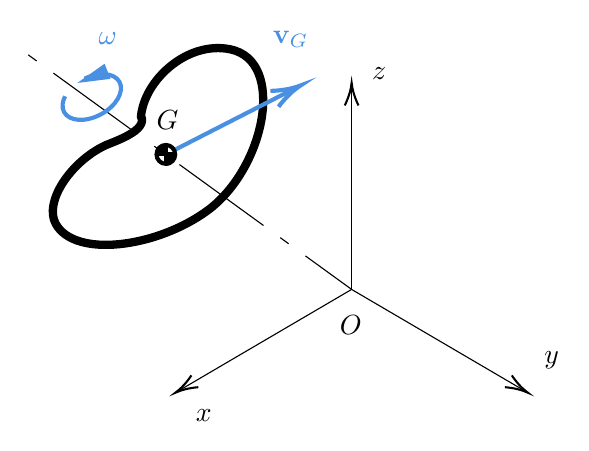
\begin{tikzpicture}[x=0.75pt,y=0.75pt,yscale=-1,xscale=1]
    \draw [color={rgb, 255:red, 0; green, 0; blue, 0 }  ,draw opacity=1 ]   (379.99,208.64) -- (379.99,111.06) ;
    \draw [shift={(379.99,109.06)}, rotate = 90] [color={rgb, 255:red, 0; green, 0; blue, 0 }  ,draw opacity=1 ][line width=0.75]    (10.93,-3.29) .. controls (6.95,-1.4) and (3.31,-0.3) .. (0,0) .. controls (3.31,0.3) and (6.95,1.4) .. (10.93,3.29)   ;
    \draw [color={rgb, 255:red, 0; green, 0; blue, 0 }  ,draw opacity=1 ]   (379.98,208.64) -- (463.22,257.42) ;
    \draw [shift={(464.94,258.43)}, rotate = 210.37] [color={rgb, 255:red, 0; green, 0; blue, 0 }  ,draw opacity=1 ][line width=0.75]    (10.93,-3.29) .. controls (6.95,-1.4) and (3.31,-0.3) .. (0,0) .. controls (3.31,0.3) and (6.95,1.4) .. (10.93,3.29)   ;
    \draw [color={rgb, 255:red, 0; green, 0; blue, 0 }  ,draw opacity=1 ]   (379.99,208.64) -- (338.26,233.09) -- (296.75,257.42) ;
    \draw [shift={(295.03,258.43)}, rotate = 329.63] [color={rgb, 255:red, 0; green, 0; blue, 0 }  ,draw opacity=1 ][line width=0.75]    (10.93,-3.29) .. controls (6.95,-1.4) and (3.31,-0.3) .. (0,0) .. controls (3.31,0.3) and (6.95,1.4) .. (10.93,3.29)   ;
    \draw  [line width=3] [line join = round][line cap = round] (278.46,125.78) .. controls (279.81,107.79) and (300.93,88.72) .. (321.49,92.95) .. controls (348.63,98.54) and (338.39,150.24) .. (310.57,170.62) .. controls (286.05,188.57) and (246.65,193.72) .. (237.42,177.02) .. controls (231.68,166.64) and (244.3,147.49) .. (261,139.39) .. controls (264.29,137.79) and (282.45,132.22) .. (278.45,124.98) ;
    \draw [color={rgb, 255:red, 0; green, 0; blue, 0 }  ,draw opacity=1 ] [dash pattern={on 3.75pt off 7.5pt on 37.5pt off 7.5pt}]  (224.18,95.63) -- (379.99,208.64) ;
    \draw  [draw opacity=0][line width=1.5]  (247.83,109.17) .. controls (250.15,107.51) and (252.87,106.21) .. (255.73,105.49) .. controls (263.49,103.53) and (269.36,106.62) .. (268.84,112.38) .. controls (268.32,118.15) and (261.61,124.41) .. (253.85,126.36) .. controls (246.09,128.32) and (240.22,125.23) .. (240.74,119.46) .. controls (240.85,118.18) and (241.28,116.87) .. (241.95,115.59) -- (254.79,115.92) -- cycle ; \draw [color={rgb, 255:red, 74; green, 144; blue, 226 }  ,draw opacity=1 ][line width=1.5]    (251.3,107.11) .. controls (252.71,106.43) and (254.2,105.87) .. (255.73,105.49) .. controls (263.49,103.53) and (269.36,106.62) .. (268.84,112.38) .. controls (268.32,118.15) and (261.61,124.41) .. (253.85,126.36) .. controls (246.09,128.32) and (240.22,125.23) .. (240.74,119.46) .. controls (240.85,118.18) and (241.28,116.87) .. (241.95,115.59) ;  \draw [shift={(247.83,109.17)}, rotate = 338.9] [fill={rgb, 255:red, 74; green, 144; blue, 226 }  ,fill opacity=1 ][line width=0.08]  [draw opacity=0] (15.6,-3.9) -- (0,0) -- (15.6,3.9) -- cycle    ;
    \draw [color={rgb, 255:red, 74; green, 144; blue, 226 }  ,draw opacity=1 ][line width=1.5]    (290.49,143.59) -- (352.8,111.71) ;
    \draw [shift={(355.47,110.34)}, rotate = 152.9] [color={rgb, 255:red, 74; green, 144; blue, 226 }  ,draw opacity=1 ][line width=1.5]    (14.21,-4.28) .. controls (9.04,-1.82) and (4.3,-0.39) .. (0,0) .. controls (4.3,0.39) and (9.04,1.82) .. (14.21,4.28)   ;
    \draw  [fill={rgb, 255:red, 255; green, 255; blue, 255 }  ,fill opacity=1 ][line width=1.5]  (286,143.59) .. controls (286,141.08) and (288.01,139.05) .. (290.49,139.05) .. controls (292.97,139.05) and (294.98,141.08) .. (294.98,143.59) .. controls (294.98,146.11) and (292.97,148.14) .. (290.49,148.14) .. controls (288.01,148.14) and (286,146.11) .. (286,143.59) -- cycle ; \draw  [line width=1.5]  (286,143.59) -- (294.98,143.59) ; \draw  [line width=1.5]  (290.49,139.05) -- (290.49,148.14) ;
    \draw  [line width=1.5] [line join = round][line cap = round] (291.1,144.08) .. controls (291.08,144.33) and (290.95,145.06) .. (290.95,144.81) .. controls (290.95,144.68) and (292.23,144.26) .. (292.33,143.87) .. controls (292.4,143.61) and (291.1,144.52) .. (291.26,144.5) .. controls (293.37,144.21) and (291.1,144.3) .. (290.95,145.38) .. controls (290.93,145.54) and (291.87,144.86) .. (291.98,144.81) .. controls (292.53,144.55) and (293.15,144.38) .. (293.62,143.98) .. controls (293.72,143.88) and (293.34,144.04) .. (293.21,144.08) .. controls (293,144.14) and (291.91,144.35) .. (292.08,144.6) .. controls (292.21,144.81) and (293.92,143.43) .. (293.82,144.29) .. controls (293.78,144.71) and (293.08,144.66) .. (292.69,144.81) .. controls (292.63,144.83) and (292.78,144.69) .. (292.85,144.65) .. controls (293.22,144.45) and (293.84,143.99) .. (294.08,144.34) .. controls (294.32,144.7) and (293.99,145.76) .. (293.41,145.17) .. controls (293.21,144.97) and (293.48,144.05) .. (293.87,144.39) .. controls (294.89,145.27) and (293.81,145.21) .. (293.67,145.02) .. controls (293.17,144.35) and (294.72,143.86) .. (294.75,144.03) .. controls (294.81,144.4) and (294.06,144.46) .. (293.93,144.81) .. controls (293.82,145.08) and (293.96,145.41) .. (293.87,145.69) .. controls (293.77,146.05) and (293.51,146.34) .. (293.36,146.68) .. controls (293.31,146.8) and (293.24,147.17) .. (293.26,147.04) .. controls (293.47,145.89) and (293.63,144.5) .. (294.28,143.51) .. controls (294.6,143.03) and (293.78,144.54) .. (293.46,145.02) .. controls (293.23,145.37) and (292.44,146.34) .. (292.75,146.06) .. controls (295.14,143.85) and (293.15,145.8) .. (292.54,146.42) .. controls (292.32,146.64) and (292.81,145.86) .. (292.95,145.59) .. controls (293.06,145.37) and (293.25,145.19) .. (293.36,144.97) .. controls (293.44,144.8) and (293.16,145.28) .. (293.05,145.43) .. controls (292.7,145.92) and (292.28,146.36) .. (291.92,146.84) .. controls (291.88,146.9) and (291.45,147.82) .. (291.15,147.67) .. controls (291.05,147.62) and (291.67,145.71) .. (292.18,145.54) .. controls (292.33,145.49) and (292.06,145.83) .. (291.98,145.95) .. controls (291.51,146.63) and (290.91,147.2) .. (290.44,147.88) .. controls (290.4,147.92) and (290.57,147.88) .. (290.59,147.82) .. controls (290.8,147.16) and (290.96,146.48) .. (291.1,145.8) .. controls (291.14,145.61) and (291.09,145.04) .. (291.15,145.23) .. controls (291.24,145.47) and (291.12,146.26) .. (291.1,146.01) .. controls (291.08,145.7) and (291.07,145.02) .. (291.36,145.12) .. controls (291.89,145.3) and (291.57,146.54) .. (291.57,146.63) .. controls (291.56,146.77) and (291.42,146.35) .. (291.46,146.21) .. controls (291.59,145.77) and (291.79,145.35) .. (291.92,144.91) .. controls (291.94,144.85) and (291.84,145.01) .. (291.82,145.07) .. controls (291.75,145.34) and (291.77,145.64) .. (291.67,145.9) .. controls (291.51,146.32) and (291.4,146.81) .. (291.05,147.1) .. controls (290.87,147.25) and (291.02,146.6) .. (291.1,146.37) .. controls (291.17,146.2) and (292.17,145.23) .. (292.08,145.28) .. controls (291.59,145.52) and (291.41,146.4) .. (291.41,146.94) .. controls (291.41,146.98) and (291.42,147.04) .. (291.46,147.04) .. controls (291.51,147.04) and (291.54,146.99) .. (291.57,146.94) .. controls (291.91,146.19) and (292.2,145.53) .. (292.69,144.86) .. controls (292.75,144.79) and (292.57,144.99) .. (292.54,145.07) .. controls (292.27,145.72) and (292.09,146.5) .. (291.67,147.1) .. controls (291.63,147.15) and (291.64,146.95) .. (291.67,146.89) .. controls (291.83,146.56) and (292.01,146.24) .. (292.23,145.95) .. controls (292.44,145.68) and (292.74,145.5) .. (292.95,145.23) .. controls (293,145.16) and (292.94,144.89) .. (292.9,144.97) .. controls (292.56,145.6) and (292.25,146.26) .. (291.82,146.84) .. controls (291.6,147.13) and (290.9,147.97) .. (291.1,147.67) .. controls (291.86,146.52) and (292.02,146.69) .. (293.1,145.8) .. controls (293.16,145.75) and (292.94,145.84) .. (292.9,145.9) .. controls (292.8,146.05) and (292.74,146.22) .. (292.64,146.37) .. controls (292.2,147.03) and (291.56,147.52) .. (291,148.08) .. controls (290.3,148.8) and (292.67,146.98) .. (293.41,146.32) .. controls (293.57,146.17) and (293.89,145.61) .. (293.72,145.75) .. controls (292.81,146.44) and (292.05,147.32) .. (291.15,148.03) .. controls (291.08,148.09) and (291.34,147.95) .. (291.41,147.88) .. controls (291.73,147.56) and (292,147.19) .. (292.33,146.89) .. controls (292.7,146.57) and (294.03,146.02) .. (294.03,145.23) .. controls (294.03,145.11) and (293.87,145.22) .. (293.87,145.23) .. controls (293.52,145.69) and (292.15,147.54) .. (291.98,147.1) .. controls (291.76,146.55) and (291.98,145.92) .. (292.03,145.33) .. controls (292.04,145.1) and (291.87,144.81) .. (292.03,144.65) ;
    \draw  [line width=1.5] [line join = round][line cap = round] (292.23,145.07) .. controls (292.19,144.85) and (292.18,144.6) .. (292.03,144.45) ;
    \draw  [line width=1.5] [line join = round][line cap = round] (286.23,142.99) .. controls (287.32,142.97) and (288.42,142.98) .. (289.51,142.94) .. controls (289.75,142.93) and (290.19,143.08) .. (290.23,142.83) .. controls (290.43,141.78) and (290.22,140.68) .. (290.13,139.61) .. controls (290.07,138.99) and (289.36,139.84) .. (289.31,139.87) .. controls (287.99,140.67) and (287.72,140.85) .. (287.1,142.05) .. controls (286.96,142.32) and (286.37,142.7) .. (286.64,142.83) .. controls (287.32,143.18) and (287.39,142.66) .. (288.02,142.57) .. controls (288.58,142.5) and (289.15,142.61) .. (289.72,142.57) .. controls (290.08,142.55) and (289.64,141.85) .. (289.67,141.48) .. controls (289.7,140.89) and (290.11,140.26) .. (289.87,139.72) .. controls (289.73,139.4) and (289.53,140.34) .. (289.26,140.55) .. controls (288.81,140.89) and (288.14,140.91) .. (287.77,141.33) .. controls (287.43,141.71) and (287.43,142.3) .. (287.25,142.78) .. controls (287.23,142.85) and (287.26,142.63) .. (287.31,142.57) .. controls (287.51,142.3) and (287.78,142.08) .. (287.97,141.79) .. controls (288.33,141.26) and (288.78,140.78) .. (289.26,140.34) .. controls (289.31,140.29) and (289.11,140.31) .. (289.05,140.34) .. controls (288.69,140.52) and (288.29,140.66) .. (288.02,140.96) .. controls (287.57,141.48) and (286.41,142.3) .. (286.95,142.73) .. controls (287.63,143.29) and (289.74,140.45) .. (289.97,140.18) .. controls (290.03,140.13) and (289.93,140.34) .. (289.87,140.39) .. controls (289.58,140.66) and (288.02,141.39) .. (288.02,142.31) .. controls (288.02,142.9) and (288.8,141.43) .. (289.26,141.07) .. controls (289.38,140.97) and (289.25,141.41) .. (289.15,141.53) .. controls (288.9,141.89) and (287.97,142.21) .. (288.28,142.52) .. controls (288.6,142.84) and (289.06,142.08) .. (289.41,141.79) .. controls (289.46,141.75) and (289.25,141.79) .. (289.2,141.85) .. controls (288.95,142.19) and (288.77,142.58) .. (288.54,142.94) .. controls (288.53,142.95) and (288.47,142.94) .. (288.49,142.94) .. controls (289.11,142.94) and (290.38,141.31) .. (289.97,141.79) .. controls (289.65,142.18) and (288.65,142.58) .. (289,142.94) .. controls (289.32,143.27) and (289.63,142.26) .. (289.97,141.95) .. controls (290.04,141.89) and (290,142.13) .. (289.97,142.21) .. controls (289.93,142.41) and (289.77,142.58) .. (289.77,142.78) .. controls (289.77,142.88) and (289.88,142.57) .. (289.97,142.57) .. controls (290.22,142.57) and (290.36,143.12) .. (290.18,143.3) ;
    \draw  [line width=1.5] [line join = round][line cap = round] (290.08,141.22) .. controls (289.92,141.33) and (289.77,141.43) .. (289.62,141.53) ;
    \draw  [line width=1.5] [line join = round][line cap = round] (286.84,140.81) .. controls (287.22,140.87) and (287.1,141.57) .. (287.05,141.95) .. controls (287.04,141.98) and (287.03,142.08) .. (287.05,142.05) .. controls (287.33,141.77) and (287.24,141.64) .. (287.41,141.27) .. controls (287.48,141.13) and (287.59,141.01) .. (287.67,140.86) .. controls (287.71,140.77) and (287.9,140.54) .. (287.82,140.6) .. controls (287.46,140.89) and (287.18,141.18) .. (286.79,141.43) ;
    \draw (303.64,265.06) node [anchor=north west][inner sep=0.75pt]  [color={rgb, 255:red, 0; green, 0; blue, 0 }  ,opacity=1 ]  {$x$};
    \draw (471.61,237.21) node [anchor=north west][inner sep=0.75pt]  [color={rgb, 255:red, 0; green, 0; blue, 0 }  ,opacity=1 ]  {$y$};
    \draw (388.63,100.33) node [anchor=north west][inner sep=0.75pt]  [color={rgb, 255:red, 0; green, 0; blue, 0 }  ,opacity=1 ]  {$z$};
    \draw (373.1,219.89) node [anchor=north west][inner sep=0.75pt]    {$O$};
    \draw (256.8,83.8) node [anchor=north west][inner sep=0.75pt]  [color={rgb, 255:red, 74; green, 144; blue, 226 }  ,opacity=1 ]  {$\omega $};
    \draw (340.8,82.8) node [anchor=north west][inner sep=0.75pt]  [color={rgb, 255:red, 74; green, 144; blue, 226 }  ,opacity=1 ]  {$\mathbf{v}_{G}$};
    \draw (284.8,121.3) node [anchor=north west][inner sep=0.75pt]    {$G$};
\end{tikzpicture}

\end{figure}

In the case of a rigid body, the velocity of a point $G$ attached to the body with respect to an intertial reference frame attached to an arbitrary point $O$ in the space can be generally expressed by its angular component $\omega$ measured and expressed in the frame $O$ about an axis passing through $O$ and its linear component $v _A$, for which the following relation holds:

\begin{equation}
    v _A = {}^O \omega \times {}^O R_G
\end{equation}

where ${}^O R_G$ is the position vector of $G$ with respect to $O$. This holds for any point $G$ on the rigid body. In order to simplify the notation, introducing a Cartesian coordinate frame $\mathcal{O} _{xyz}$, we can define a basis of 6 spatial vectors $\mathcal{D} _O = \{\mathbf{d} _i\} ^6 _{i=1}$ as:

\begin{equation}
    \mathcal{D} _O = \{\mathbf{d} _x, \mathbf{d} _y, \mathbf{d} _z, \mathbf{d} _{O _x}, \mathbf{d} _{O _y}, \mathbf{d} _{O _z} \} \subset \mathcal{M} ^6
\end{equation}

where $\mathcal{M} ^6$ is the space of 6D vectors, defining a Pl\"ucker coordinate system on $\mathcal{M} ^6$ as shown in \cref{fig:pluecker}.

% === Fig: Pluecker === %
\begin{figure}
    \centering
    \caption{Pl\"ucker Motion Coordinate System.}
    \label{fig:pluecker}
    \tikzset{every picture/.style={line width=0.75pt}}
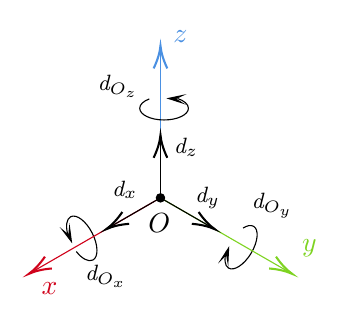
\begin{tikzpicture}[x=0.75pt,y=0.75pt,yscale=-1,xscale=1]
    \draw [color={rgb, 255:red, 74; green, 144; blue, 226 }  ,draw opacity=1 ]   (249.79,80.38) -- (249.79,9.08) ;
    \draw [shift={(249.79,7.08)}, rotate = 90] [color={rgb, 255:red, 74; green, 144; blue, 226 }  ,draw opacity=1 ][line width=0.75]    (10.93,-3.29) .. controls (6.95,-1.4) and (3.31,-0.3) .. (0,0) .. controls (3.31,0.3) and (6.95,1.4) .. (10.93,3.29)   ;
    \draw  [draw opacity=0] (257.99,32.5) .. controls (261.16,33.51) and (263.25,35.24) .. (263.25,37.21) .. controls (263.25,40.32) and (258,42.85) .. (251.52,42.85) .. controls (245.05,42.85) and (239.8,40.32) .. (239.8,37.21) .. controls (239.8,35.38) and (241.61,33.75) .. (244.41,32.72) -- (251.52,37.21) -- cycle ; \draw   (257.99,32.5) .. controls (261.16,33.51) and (263.25,35.24) .. (263.25,37.21) .. controls (263.25,40.32) and (258,42.85) .. (251.52,42.85) .. controls (245.05,42.85) and (239.8,40.32) .. (239.8,37.21) .. controls (239.8,35.38) and (241.61,33.75) .. (244.41,32.72) ;
    \draw  [draw opacity=0] (205.05,97.73) .. controls (204.06,93.79) and (204.55,90.48) .. (206.55,89.46) .. controls (209.33,88.05) and (213.96,91.58) .. (216.9,97.35) .. controls (219.84,103.12) and (219.97,108.94) .. (217.19,110.35) .. controls (215.09,111.42) and (211.93,109.66) .. (209.25,106.25) -- (211.87,99.91) -- cycle ; \draw   (205.05,97.73) .. controls (204.06,93.79) and (204.55,90.48) .. (206.55,89.46) .. controls (209.33,88.05) and (213.96,91.58) .. (216.9,97.35) .. controls (219.84,103.12) and (219.97,108.94) .. (217.19,110.35) .. controls (215.09,111.42) and (211.93,109.66) .. (209.25,106.25) ;
    \draw  [draw opacity=0] (289.6,94.92) .. controls (291.53,93.69) and (293.37,93.33) .. (294.68,94.12) .. controls (297.34,95.72) and (296.8,101.52) .. (293.45,107.07) .. controls (290.11,112.61) and (285.24,115.81) .. (282.57,114.2) .. controls (280.67,113.05) and (280.4,109.78) .. (281.61,105.98) -- (288.62,104.16) -- cycle ; \draw   (289.6,94.92) .. controls (291.53,93.69) and (293.37,93.33) .. (294.68,94.12) .. controls (297.34,95.72) and (296.8,101.52) .. (293.45,107.07) .. controls (290.11,112.61) and (285.24,115.81) .. (282.57,114.2) .. controls (280.67,113.05) and (280.4,109.78) .. (281.61,105.98) ;
    \draw  [fill={rgb, 255:red, 0; green, 0; blue, 0 }  ,fill opacity=1 ] (205.98,94.78) -- (206.86,101.37) -- (202.81,96.09) -- (205.63,98.4) -- cycle ;
    \draw  [fill={rgb, 255:red, 0; green, 0; blue, 0 }  ,fill opacity=1 ] (279.01,110.18) -- (282.61,104.59) -- (282.28,111.23) -- (281.63,107.65) -- cycle ;
    \draw  [fill={rgb, 255:red, 0; green, 0; blue, 0 }  ,fill opacity=1 ] (260,34.53) -- (253.67,32.48) -- (260.18,31.11) -- (256.88,32.65) -- cycle ;
    \draw [color={rgb, 255:red, 126; green, 211; blue, 33 }  ,draw opacity=1 ]   (249.79,80.38) -- (311.53,116.02) ;
    \draw [shift={(313.27,117.02)}, rotate = 210] [color={rgb, 255:red, 126; green, 211; blue, 33 }  ,draw opacity=1 ][line width=0.75]    (10.93,-3.29) .. controls (6.95,-1.4) and (3.31,-0.3) .. (0,0) .. controls (3.31,0.3) and (6.95,1.4) .. (10.93,3.29)   ;
    \draw [color={rgb, 255:red, 208; green, 2; blue, 27 }  ,draw opacity=1 ]   (249.79,80.37) -- (218.61,98.38) -- (188.04,116.02) ;
    \draw [shift={(186.31,117.02)}, rotate = 330] [color={rgb, 255:red, 208; green, 2; blue, 27 }  ,draw opacity=1 ][line width=0.75]    (10.93,-3.29) .. controls (6.95,-1.4) and (3.31,-0.3) .. (0,0) .. controls (3.31,0.3) and (6.95,1.4) .. (10.93,3.29)   ;
    \draw    (249.79,80.38) -- (249.79,52.13) ;
    \draw [shift={(249.79,50.13)}, rotate = 90] [color={rgb, 255:red, 0; green, 0; blue, 0 }  ][line width=0.75]    (10.93,-3.29) .. controls (6.95,-1.4) and (3.31,-0.3) .. (0,0) .. controls (3.31,0.3) and (6.95,1.4) .. (10.93,3.29)   ;
    \draw    (249.79,80.38) -- (274.25,94.5) ;
    \draw [shift={(275.99,95.5)}, rotate = 210] [color={rgb, 255:red, 0; green, 0; blue, 0 }  ][line width=0.75]    (10.93,-3.29) .. controls (6.95,-1.4) and (3.31,-0.3) .. (0,0) .. controls (3.31,0.3) and (6.95,1.4) .. (10.93,3.29)   ;
    \draw    (249.79,80.37) -- (225.32,94.5) ;
    \draw [shift={(223.59,95.5)}, rotate = 330] [color={rgb, 255:red, 0; green, 0; blue, 0 }  ][line width=0.75]    (10.93,-3.29) .. controls (6.95,-1.4) and (3.31,-0.3) .. (0,0) .. controls (3.31,0.3) and (6.95,1.4) .. (10.93,3.29)   ;
    \draw (191.23,119.9) node [anchor=north west][inner sep=0.75pt]  [color={rgb, 255:red, 208; green, 2; blue, 27 }  ,opacity=1 ]  {$x$};
    \draw (316.73,99.4) node [anchor=north west][inner sep=0.75pt]  [color={rgb, 255:red, 126; green, 211; blue, 33 }  ,opacity=1 ]  {$y$};
    \draw (254.73,-1.35) node [anchor=north west][inner sep=0.75pt]  [color={rgb, 255:red, 74; green, 144; blue, 226 }  ,opacity=1 ]  {$z$};
    \draw (212.25,111.65) node [anchor=north west][inner sep=0.75pt]  [font=\footnotesize]  {$\mathit{d}_{O_{x}}$};
    \draw (218.25,20.15) node [anchor=north west][inner sep=0.75pt]  [font=\footnotesize]  {$\mathit{d}_{O_{z}}$};
    \draw (292.5,76.9) node [anchor=north west][inner sep=0.75pt]  [font=\footnotesize]  {$\mathit{d}_{O_{y}}$};
    \draw (255,50.4) node [anchor=north west][inner sep=0.75pt]  [font=\footnotesize]  {$\mathit{d}_{z}$};
    \draw (225.25,70.9) node [anchor=north west][inner sep=0.75pt]  [font=\footnotesize]  {$\mathit{d}_{x}$};
    \draw (265.25,73.9) node [anchor=north west][inner sep=0.75pt]  [font=\footnotesize]  {$\mathit{d}_{y}$};
    \draw (242.75,86.65) node [anchor=north west][inner sep=0.75pt]    {$O$};
    \draw [fill={rgb, 255:red, 0; green, 0; blue, 0 }  ,fill opacity=1 ]  (249.79, 80.38) circle [x radius= 2, y radius= 2]   ;
\end{tikzpicture}
\end{figure}

\paragraph{Spatial Subspace} Once defined $\mathcal{M} ^n$ as a vector space, we can define a subset $\boldsymbol{\Phi} \subset \mathcal{M} ^n$, which is also a vector space. Given a constraint matrix $\mathbf{K} \in \mathbb{R} ^{m \times n}$ with $m$ number of constraints and $n$ number of degrees of freedom, then we can define the subspace $\boldsymbol{\Phi}$ as the null space of $\mathbf{K}$:

\begin{equation}
    \boldsymbol{\Phi} = \ker (\mathbf{K})
\end{equation}

This defines a motion subspace for a system, e.g. defines the directions in which the system is free to move.

\paragraph{Spatial Velocity} The spatial velocity of a rigid body is defined as a serialization of the linear and angular velocity of a point $A$ attached to the body. In particular, let $\mathbf{p} _A \in \mathcal{D}_O$ be the pose vector of $A$ with respect to $O$, then the spatial velocity of the body is defined as the component-wise derivative of the spatial vector respect to time:

\begin{equation}
    \mathbf{v} _A = \frac{d}{dt} {}^{[O]}\mathbf{p} _A =
    \lim _{\delta t \to 0} \frac{1}{\delta t}
    \begin{bmatrix}
        p _{A _x} (t + \delta t)     & - & p _{A _x} (t)     \\
        p _{A _y} (t + \delta t)     & - & p _{A _y} (t)     \\
        p _{A _z} (t + \delta t)     & - & p _{A _z} (t)     \\
        p _{A _{O_x}} (t + \delta t) & - & p _{A _{O_x}} (t) \\
        p _{A _{O_y}} (t + \delta t) & - & p _{A _{O_y}} (t) \\
        p _{A _{O_z}} (t + \delta t) & - & p _{A _{O_z}} (t) \\
    \end{bmatrix}
    = \begin{bmatrix}
        v _A \\
        \omega _A
    \end{bmatrix}
\end{equation}

\paragraph{Spatial Acceleration} Given that the spatial velocity decouples the linear and angular components of the motion, defining a property of the body as a whole and not of a single body-fixed point, the spatial acceleration of a rigid body is defined as simply as just the time derivative of its spatial velocity:

\begin{equation}
    \dot{\mathbf{v}} _A = \frac{d}{dt} \begin{bmatrix}
        v _A (t) \\
        \omega (t)
    \end{bmatrix}
    =
    \begin{bmatrix}
        \dot{v} _A \\
        \dot{\omega}
    \end{bmatrix}
\end{equation}

\paragraph{Spatial Forces} The spatial force acting on a rigid body is defined, in a similar manner as the spatial velocity as a stacking of the linear component $f \in \mathbb{R}^3$ and the angular component $\tau \in \mathbb{R}^3$ of the wrench acting on the body, in particular, we can defined $\mathbf{f} \in \mathbb{R}^6$ respect to a frame $B$ in relation to its motion as:

\begin{equation}
    {}_{B}\mathbf{f} = \begin{bmatrix}
        {}_{B}f \\
        {}_{B}\tau
    \end{bmatrix}
\end{equation}

\paragraph{Multibody Velocity} Given a floating-base multibody system composed of $n$ rigid bodies, we can define the velocity of the system as the concatenation of the root link velocity $\mathbf{v}_A$ and the velocities of each body composing the system $\dot{\mathbf{s}} \in \mathbb{R} ^{n}$:

\begin{equation}
    \boldsymbol{\nu} = \begin{bmatrix}
        \begin{bmatrix} v _a \\ \omega _A \end{bmatrix} \\
        \dot{\mathbf{s}}                                \\
    \end{bmatrix} = \begin{bmatrix}
        \mathbf{v}_A \\
        \dot{\mathbf{s}}
    \end{bmatrix}
\end{equation}

\paragraph{Multibody Acceleration} Similarly, the acceleration of the floating-base system can be defined as the concatenation of the acceleration of the root link $\dot{\mathbf{v}} _A$ and the accelerations of each body composing the system $\ddot{\mathbf{s}} \in \mathbb{R} ^{n}$:

\begin{equation}
    \dot{\boldsymbol{\nu _A}} = \begin{bmatrix}
        \begin{bmatrix} \dot{v} _a \\ \dot{\omega} _A \end{bmatrix} \\
        \ddot{\mathbf{s}}                                           \\
    \end{bmatrix} = \begin{bmatrix}
        \dot{\mathbf{v}}_A \\
        \ddot{\mathbf{s}}
    \end{bmatrix}
\end{equation}

\section{Multibody Kinematics}

\subsection{Joints and Links}

A multibody kinematic tree can be described as a contiguous assembly of two main physical elements: links and joints. The links correspond to the rigid bodies composing the inertial properties of the system, while the joints are usually modeled as massless elements connecting two links, allowing relative motion between them. They are classified according to the number of \ac{DoF} they allow, which is the number of independent coordinates needed to describe the relative motion between the two links, usually assuming values between 0 (fixed joint) and 6 (free joint).

For the sake of simplicity and without loss of generality, in this work, only 1-\ac{DoF} joint will be considered, as their properties can be easily extended to multidimensional cases. Furthermore, the system will be considered \textit{acyclic}, i.e. it will not contain any closed loop, as the presence of loops would make the system kinematically redundant.
Given a joint we can define a \textit{joint axis} $\mathbf{a} \in \mathbb{R}^3, |\mathbf{a}| = 1$ with $\mathbf{a}^\wedge \mathbf{a} = \mathbbm{0}_{3 \times 1}$, in this case, if we recall the definition of the spatial subspace, we can define the joint motion subspace $\boldsymbol{\Phi} _j \in \mathcal{M} ^6$ as:

\begin{equation}
    \boldsymbol{\Phi} _j =
    \begin{cases}
        [\mathbbm{0}_{1 \times 6}] ^\top             & \text{if the joint is fixed}     \\
        [\mathbf{a}, \mathbbm{0}_{1 \times 3}] ^\top & \text{if the joint is prismatic} \\
        [\mathbbm{0}_{1 \times 3}, \mathbf{a}] ^\top & \text{if the joint is revolute}
    \end{cases}
\end{equation}

\section{Equation of Motion}
\label{sec:back_eom}

When dealing with a multi-body system, the configuration must be described in non-Euclidean space by a configuration belonging to a smooth manifold ${}^W\mathbf{H} \in \mathbb{Q}:\mathrm{SE}(3)\times\mathbb{R}^n$ where $H$ is the pose of the system and $n$ is the number of \ac{DoF} of the system and $\mathrm{SE}(3)$ is the \textit{special Euclidean} Lie group defined as:

\begin{equation}
    \mathrm{SE}(3) := \left\{
    \begin{bmatrix}
        \mathbf{R}                & \mathbf{p} \\
        \mathbbm{0} _{1 \times 3} & 1
    \end{bmatrix} \in \mathbb{R} ^4 \mid \mathbf{R} \in \mathrm{SO}(3), \mathbf{p} \in \mathbb{R} ^3
    \right\}
\end{equation}

and $\mathrm{SO}(3)$ is the \textit{special orthogonal} Lie group defined as:

\begin{equation}
    \mathrm{SO}(3) := \left\{
    \mathbf{R} \in \mathbb{R} ^{3 \times 3} \mid \mathbf{R} ^\top \mathbf{R} = \mathbb{I}, \det(R) = 1
    \right\}
\end{equation}

The derivative of the pose ${}^W\dot{\mathbf{H}}$ is a vector belonging to the tangent space of $\mathbb{Q}$, i.e. ${}^W\dot{\mathbf{H}} \in \mathbb{T} _{\mathbb{G}} \mathbb{Q}$:

\begin{equation}
    \mathbb{T} _{\mathbb{G}} \mathbb{Q} := \left\{
    \begin{bmatrix}
        \mathbf{S}                & \mathbf{v} \\
        \mathbbm{0} _{1 \times 3} & 0
    \end{bmatrix} \in \mathbb{R} ^6 \mid \mathbf{S} \in \mathfrak{so}(3), \mathbf{v} \in \mathbb{R} ^3
    \right\}
\end{equation}

where $\mathfrak{so}(3)$ is the \textit{special orthogonal} Lie algebra of $\mathrm{SO}(3)$, defined as the set of $3\times3$ skew-symmetric matrices:

\begin{equation}
    \mathfrak{so}(3) = \{S \in \mathbb{R}^{3\times3} \mid S^\top = -S \}
\end{equation}

The equation of motion of a generic multibody mechanical system can be derived starting from the Principle of Least Action, which states that in a time interval $[t _0, t _1]$ the motion of a system is such that the action functional $\mathcal{A}$ is stationary, i.e. the first variation of the action functional is zero:

\begin{equation}
    \mathcal{A} = \int _{t _0} ^{t _1} \mathcal{L} (\mathbf{q}(t), \mathbf{\dot{q}}(t)) dt \quad \text{with } \delta \mathcal{A} = 0
\end{equation}

where $\mathcal{L} (\mathbf{q} = {}^W\mathbf{H} _B, \dot{\mathbf{q}} = {}^W\dot{\mathbf{H}} _B)$ is the Lagrangian of the system. For a floating-base multibody system, it can be obtained as the sum of the Lagrangian of each link composing the system:

\begin{equation}
    \mathcal{L} = \mathcal{T}(\mathbf{q},\boldsymbol{\nu}) - \mathcal{U}(\mathbf{q}) = \sum _{L \in \mathbb{L}} \mathrm{v} ^\top _L \mathbb{M} _L \mathrm{v} _L - \sum _{L \in \mathbb{L}} \begin{bmatrix}
        \mathbf{g} ^\top _L & \mathbbm{0}
    \end{bmatrix} {}^W\mathbf{H} _L
    \begin{bmatrix}
        m _L c _L \\ m _L
    \end{bmatrix}
\end{equation}

where $\mathbb{L}$ is the set of links composing the system, $\mathbb{M} _L \in \mathbb{R} ^{6 \times 6}$ is the spatial inertia matrix of the link $L$, $\mathbf{g} _L$ is the gravitational acceleration vector, ${}^W\mathbf{H} _L \in \mathbb{Q}$ is the pose of the link $L$ and $m _L \in \mathbb{R}$ and $c _L \in \mathbb{R}$ are the mass and the Coriolis acceleration

The first variation of the action functional can be written as:

\begin{equation}
    \delta \mathcal{A} = \int _{t _0} ^{t _1} \delta \mathcal{L} (\mathbf{q}(t), \mathbf{\dot{q}}(t))dt = \int _{t _0} ^{t _1} \left( \frac{\partial \mathcal{L}}{\partial \mathbf{q}} \delta \mathbf{q} + \frac{\partial \mathcal{L}}{\partial \mathbf{\dot{q}}} \delta \mathbf{\dot{q}} \right) dt
\end{equation}

where $\delta \mathbf{q}$ and $\delta \mathbf{\dot{q}}$ are the variations of the generalized coordinates and velocities, respectively. The first variation of the action functional is zero if and only if the integrand is zero. In the case of Euclidean spaces, i.e. $\mathbb{Q} = \mathbb{T} _{\mathbb{G}}\mathbb{Q} =\mathbb{R} ^n$, this yields the Euler-Lagrange equation:

\begin{equation}
    \frac{d}{dt} \frac{\partial \mathcal{L}}{\partial \mathbf{\dot{q}}} - \frac{\partial \mathcal{L}}{\partial \mathbf{q}} = 0
    \label{eqn:lagrangian}
\end{equation}

The following chapters will always consider a rigid body pose and body-fixed velocities, thus yielding the \textit{left-trivialized Lagrangian} \citep{traversaro_modelling_2019}:

\begin{equation}
    l(\mathbf{H}, \boldsymbol{\nu}) = \mathcal{L}(\mathbf{H}, \mathbf{H}\boldsymbol{\nu}^\wedge) = \mathcal{T}(\boldsymbol{\nu}) - \mathcal{U}(\mathbf{H})
\end{equation}

in which $\boldsymbol{\nu}^\wedge$ is the skew-symmetric matrix of the body-fixed velocity $\boldsymbol{\nu}$.

Once defined a map $\mathbb{M} \in \mathbb{R}^{(6+n) \times (6+n)}$ as the generalized inertia matrix for the kinetic energy $\mathcal{T}$, a Coriolis vector $\mathbf{h} \in \mathbb{R} ^{6+n}$ including the contribution of centrifugal and gravitational forces, a selection matrix $\mathbf{B} = \begin{bmatrix} \mathbbm{0}_{n\times6} & \mathbbm{1}_n \end{bmatrix}^\top$ for the actuation torques $\boldsymbol{\tau} \in \mathbb{R} ^n$, a Jacobian matrix $\mathbf{J} _\text{c} \in \mathbb{R} ^{(6+n) \times (6+n_c)}$ for the external forces $\mathbf{F} ^\text{ext} \in \mathbb{R} ^{n_c}$ with $n_c$ number of contact frames, the equation of motion can be finally obtained \citep{SicilianoKhatib2008}:

\begin{equation}
    \label{eqn:equation_of_motion}
    \mathbb{M}(\mathbf{q}) \mathbf{\ddot{\boldsymbol{\nu}}} + \mathbf{h} (\mathbf{q}, \boldsymbol{\nu}) = \mathbf{B}\boldsymbol{\tau} + \mathbf{J}^\top _\text{c} \mathbf{F} ^\text{ext}
\end{equation}


\section{Forward Dynamics}
\label{sec:back_fd}

The forward dynamics problem consists of computing the joint accelerations of a multibody system given the joint positions, velocities, and applied forces. The computation of the acceleration of a link normally involves the inversion of the mass matrix, which can easily become huge in a multibody system with a high number of links, in fact, the mass matrix of a system with $n$ links is a $6+n \times 6+n$ matrix, as explained in \cref{sec:back_eom}. Although being algorithms involving the inertia matrix inversion much simpler to implement, propagation algorithms involving recursive backsubstition are more efficient in terms of computational cost, as they can reach the theoretical minimal complexity of $\mathcal{O}(n)$. In this work, the notation $\mathrm{FD}(\cdot)$ will be used to indicate the forward dynamics computation.

\begin{equation}
    \ddot{\mathbf{s}} = \mathrm{FD} (\mathcal{M}, \mathbf{s}, \dot{\mathbf{s}}, \boldsymbol{\tau}, \mathbf{F} ^{\text{ext}})
\end{equation}

\subsection{Articulated-Body Algorithm}
\label{subsec:back_aba}

As anticipated, the inversion of the mass matrix for a multi-body system with a high number of links is computationally expensive, in fact, even using \citet{coppersmith_matrix_1990} algorithm or its optimized version by \citet{vassilevska-williams2012breaking}, which reached a complexity of $\mathcal{O}(n^{2.373})$, the computation of the inverse of the mass matrix is still too expensive for real-time scenarios. That is why recursive methods results are more suitable for applications where a fast computation of the dynamics is required. In recursive algorithms, as the problem is unsolvable for a single body of the system, the usual approach is to define the constraints that the links must satisfy, write the equation for each link, calculate the local coefficient, and then propagate them in the kinematic tree until a point in which the problem becomes solvable, usually the base of the tree in backpropagation or the end-effector in forward propagation.

% === FIG: Kinematic Chain === %
\begin{figure}[h]
    \centering
    \caption{Kinematic subtree visualization.}
    \label{fig:kin_tree}
    \subfloat[Branched kinematic tree]{
        \resizebox{0.45\textwidth}{!}{
            \tikzset {_wvafpciex/.code = {\pgfsetadditionalshadetransform{ \pgftransformshift{\pgfpoint{0 bp } { 0 bp }  }  \pgftransformrotate{-117 }  \pgftransformscale{2 }  }}}
\pgfdeclarehorizontalshading{_sy15ycl19}{150bp}{rgb(0bp)=(1,1,1);
    rgb(37.5bp)=(1,1,1);
    rgb(50.08184160505022bp)=(0.95,0.95,0.95);
    rgb(57.64583042689732bp)=(0.88,0.88,0.88);
    rgb(61.33184160505022bp)=(0.96,0.96,0.96);
    rgb(100bp)=(0.96,0.96,0.96)}
\tikzset {_svf4mjzjm/.code = {\pgfsetadditionalshadetransform{ \pgftransformshift{\pgfpoint{0 bp } { 0 bp }  }  \pgftransformrotate{-117 }  \pgftransformscale{2 }  }}}
\pgfdeclarehorizontalshading{_e9qihdtow}{150bp}{rgb(0bp)=(1,1,1);
    rgb(37.5bp)=(1,1,1);
    rgb(50.08184160505022bp)=(0.95,0.95,0.95);
    rgb(57.64583042689732bp)=(0.88,0.88,0.88);
    rgb(61.33184160505022bp)=(0.96,0.96,0.96);
    rgb(100bp)=(0.96,0.96,0.96)}
\tikzset {_ddhli8fcf/.code = {\pgfsetadditionalshadetransform{ \pgftransformshift{\pgfpoint{0 bp } { 0 bp }  }  \pgftransformrotate{-117 }  \pgftransformscale{2 }  }}}
\pgfdeclarehorizontalshading{_bw97u0oo5}{150bp}{rgb(0bp)=(1,1,1);
    rgb(37.5bp)=(1,1,1);
    rgb(50.08184160505022bp)=(0.95,0.95,0.95);
    rgb(57.64583042689732bp)=(0.88,0.88,0.88);
    rgb(61.33184160505022bp)=(0.96,0.96,0.96);
    rgb(100bp)=(0.96,0.96,0.96)}
\tikzset {_rzri9nu6o/.code = {\pgfsetadditionalshadetransform{ \pgftransformshift{\pgfpoint{0 bp } { 0 bp }  }  \pgftransformrotate{-117 }  \pgftransformscale{2 }  }}}
\pgfdeclarehorizontalshading{_irmxrz6bl}{150bp}{rgb(0bp)=(1,1,1);
    rgb(37.5bp)=(1,1,1);
    rgb(50.08184160505022bp)=(0.95,0.95,0.95);
    rgb(57.64583042689732bp)=(0.88,0.88,0.88);
    rgb(61.33184160505022bp)=(0.96,0.96,0.96);
    rgb(100bp)=(0.96,0.96,0.96)}
\tikzset {_tv3cr0nbo/.code = {\pgfsetadditionalshadetransform{ \pgftransformshift{\pgfpoint{0 bp } { 0 bp }  }  \pgftransformrotate{-117 }  \pgftransformscale{2 }  }}}
\pgfdeclarehorizontalshading{_ria03yqfs}{150bp}{rgb(0bp)=(1,1,1);
    rgb(37.5bp)=(1,1,1);
    rgb(50.08184160505022bp)=(0.95,0.95,0.95);
    rgb(57.64583042689732bp)=(0.88,0.88,0.88);
    rgb(61.33184160505022bp)=(0.96,0.96,0.96);
    rgb(100bp)=(0.96,0.96,0.96)}
\tikzset {_0hgwncxm6/.code = {\pgfsetadditionalshadetransform{ \pgftransformshift{\pgfpoint{0 bp } { 0 bp }  }  \pgftransformrotate{-117 }  \pgftransformscale{2 }  }}}
\pgfdeclarehorizontalshading{_7fixrohbn}{150bp}{rgb(0bp)=(1,1,1);
    rgb(37.5bp)=(1,1,1);
    rgb(50.08184160505022bp)=(0.95,0.95,0.95);
    rgb(57.64583042689732bp)=(0.88,0.88,0.88);
    rgb(61.33184160505022bp)=(0.96,0.96,0.96);
    rgb(100bp)=(0.96,0.96,0.96)}
\tikzset {_te42shfqc/.code = {\pgfsetadditionalshadetransform{ \pgftransformshift{\pgfpoint{0 bp } { 0 bp }  }  \pgftransformrotate{-117 }  \pgftransformscale{2 }  }}}
\pgfdeclarehorizontalshading{_9prsrmsl7}{150bp}{rgb(0bp)=(1,1,1);
    rgb(37.5bp)=(1,1,1);
    rgb(50.08184160505022bp)=(0.95,0.95,0.95);
    rgb(57.64583042689732bp)=(0.88,0.88,0.88);
    rgb(61.33184160505022bp)=(0.96,0.96,0.96);
    rgb(100bp)=(0.96,0.96,0.96)}
\tikzset {_qoggn7fn2/.code = {\pgfsetadditionalshadetransform{ \pgftransformshift{\pgfpoint{0 bp } { 0 bp }  }  \pgftransformrotate{-117 }  \pgftransformscale{2 }  }}}
\pgfdeclarehorizontalshading{_8g14z78sd}{150bp}{rgb(0bp)=(1,1,1);
    rgb(37.5bp)=(1,1,1);
    rgb(50.08184160505022bp)=(0.95,0.95,0.95);
    rgb(57.64583042689732bp)=(0.88,0.88,0.88);
    rgb(61.33184160505022bp)=(0.96,0.96,0.96);
    rgb(100bp)=(0.96,0.96,0.96)}
\tikzset {_3ytgx3jcr/.code = {\pgfsetadditionalshadetransform{ \pgftransformshift{\pgfpoint{0 bp } { 0 bp }  }  \pgftransformrotate{-117 }  \pgftransformscale{2 }  }}}
\pgfdeclarehorizontalshading{_hjawm1m3k}{150bp}{rgb(0bp)=(1,1,1);
    rgb(37.5bp)=(1,1,1);
    rgb(50.08184160505022bp)=(0.95,0.95,0.95);
    rgb(57.64583042689732bp)=(0.88,0.88,0.88);
    rgb(61.33184160505022bp)=(0.96,0.96,0.96);
    rgb(100bp)=(0.96,0.96,0.96)}
\tikzset {_Am47npqyx/.code = {\pgfsetadditionalshadetransform{ \pgftransformshift{\pgfpoint{0 bp } { 0 bp }  }  \pgftransformrotate{-117 }  \pgftransformscale{2 }  }}}
\pgfdeclarehorizontalshading{_hbtcw454n}{150bp}{rgb(0bp)=(1,1,1);
    rgb(37.5bp)=(1,1,1);
    rgb(50.08184160505022bp)=(0.95,0.95,0.95);
    rgb(57.64583042689732bp)=(0.88,0.88,0.88);
    rgb(61.33184160505022bp)=(0.96,0.96,0.96);
    rgb(100bp)=(0.96,0.96,0.96)}
\tikzset {_igkxxgbt5/.code = {\pgfsetadditionalshadetransform{ \pgftransformshift{\pgfpoint{0 bp } { 0 bp }  }  \pgftransformrotate{-117 }  \pgftransformscale{2 }  }}}
\pgfdeclarehorizontalshading{_4ks716t6n}{150bp}{rgb(0bp)=(1,1,1);
    rgb(37.5bp)=(1,1,1);
    rgb(50.08184160505022bp)=(0.95,0.95,0.95);
    rgb(57.64583042689732bp)=(0.88,0.88,0.88);
    rgb(61.33184160505022bp)=(0.96,0.96,0.96);
    rgb(100bp)=(0.96,0.96,0.96)}
\tikzset{every picture/.style={line width=0.75pt}}
\begin{tikzpicture}[x=0.75pt,y=0.75pt,yscale=-1,xscale=1]
    \path  [shading=_sy15ycl19,_wvafpciex] (340.92,97.33) .. controls (340.92,88.96) and (364.78,82.17) .. (394.21,82.17) .. controls (423.64,82.17) and (447.5,88.96) .. (447.5,97.33) .. controls (447.5,105.71) and (423.64,112.5) .. (394.21,112.5) .. controls (364.78,112.5) and (340.92,105.71) .. (340.92,97.33) -- cycle ;
    \draw  [color={rgb, 255:red, 0; green, 0; blue, 0 }  ,draw opacity=1 ][line width=0.75]  (340.92,97.33) .. controls (340.92,88.96) and (364.78,82.17) .. (394.21,82.17) .. controls (423.64,82.17) and (447.5,88.96) .. (447.5,97.33) .. controls (447.5,105.71) and (423.64,112.5) .. (394.21,112.5) .. controls (364.78,112.5) and (340.92,105.71) .. (340.92,97.33) -- cycle ;
    \path  [shading=_e9qihdtow,_svf4mjzjm] (528.22,14.11) .. controls (534.45,19.72) and (523.53,41.99) .. (503.84,63.87) .. controls (484.15,85.75) and (463.14,98.94) .. (456.92,93.33) .. controls (450.69,87.73) and (461.61,65.45) .. (481.3,43.58) .. controls (500.99,21.7) and (522,8.51) .. (528.22,14.11) -- cycle ;
    \draw  [color={rgb, 255:red, 0; green, 0; blue, 0 }  ,draw opacity=1 ][line width=0.75]  (528.22,14.11) .. controls (534.45,19.72) and (523.53,41.99) .. (503.84,63.87) .. controls (484.15,85.75) and (463.14,98.94) .. (456.92,93.33) .. controls (450.69,87.73) and (461.61,65.45) .. (481.3,43.58) .. controls (500.99,21.7) and (522,8.51) .. (528.22,14.11) -- cycle ;
    \path  [shading=_bw97u0oo5,_ddhli8fcf] (447.5,97.33) .. controls (447.5,94.46) and (449.83,92.13) .. (452.71,92.13) .. controls (455.58,92.13) and (457.92,94.46) .. (457.92,97.33) .. controls (457.92,100.21) and (455.58,102.54) .. (452.71,102.54) .. controls (449.83,102.54) and (447.5,100.21) .. (447.5,97.33) -- cycle ;
    \draw  [color={rgb, 255:red, 0; green, 0; blue, 0 }  ,draw opacity=1 ][line width=0.75]  (447.5,97.33) .. controls (447.5,94.46) and (449.83,92.13) .. (452.71,92.13) .. controls (455.58,92.13) and (457.92,94.46) .. (457.92,97.33) .. controls (457.92,100.21) and (455.58,102.54) .. (452.71,102.54) .. controls (449.83,102.54) and (447.5,100.21) .. (447.5,97.33) -- cycle ;
    \path  [shading=_irmxrz6bl,_rzri9nu6o] (332.22,101.61) .. controls (338.45,107.22) and (327.53,129.49) .. (307.84,151.37) .. controls (288.15,173.25) and (267.14,186.44) .. (260.92,180.83) .. controls (254.69,175.23) and (265.61,152.95) .. (285.3,131.08) .. controls (304.99,109.2) and (326,96.01) .. (332.22,101.61) -- cycle ;
    \draw  [color={rgb, 255:red, 0; green, 0; blue, 0 }  ,draw opacity=1 ][line width=0.75]  (332.22,101.61) .. controls (338.45,107.22) and (327.53,129.49) .. (307.84,151.37) .. controls (288.15,173.25) and (267.14,186.44) .. (260.92,180.83) .. controls (254.69,175.23) and (265.61,152.95) .. (285.3,131.08) .. controls (304.99,109.2) and (326,96.01) .. (332.22,101.61) -- cycle ;
    \path  [shading=_ria03yqfs,_tv3cr0nbo] (330.5,97.33) .. controls (330.5,94.46) and (332.83,92.13) .. (335.71,92.13) .. controls (338.58,92.13) and (340.92,94.46) .. (340.92,97.33) .. controls (340.92,100.21) and (338.58,102.54) .. (335.71,102.54) .. controls (332.83,102.54) and (330.5,100.21) .. (330.5,97.33) -- cycle ;
    \draw  [color={rgb, 255:red, 0; green, 0; blue, 0 }  ,draw opacity=1 ][line width=0.75]  (330.5,97.33) .. controls (330.5,94.46) and (332.83,92.13) .. (335.71,92.13) .. controls (338.58,92.13) and (340.92,94.46) .. (340.92,97.33) .. controls (340.92,100.21) and (338.58,102.54) .. (335.71,102.54) .. controls (332.83,102.54) and (330.5,100.21) .. (330.5,97.33) -- cycle ;
    \path  [shading=_7fixrohbn,_0hgwncxm6] (252.46,184.96) .. controls (252.46,182.08) and (254.79,179.75) .. (257.67,179.75) .. controls (260.54,179.75) and (262.87,182.08) .. (262.87,184.96) .. controls (262.87,187.83) and (260.54,190.17) .. (257.67,190.17) .. controls (254.79,190.17) and (252.46,187.83) .. (252.46,184.96) -- cycle ;
    \draw  [color={rgb, 255:red, 0; green, 0; blue, 0 }  ,draw opacity=1 ][line width=0.75]  (252.46,184.96) .. controls (252.46,182.08) and (254.79,179.75) .. (257.67,179.75) .. controls (260.54,179.75) and (262.87,182.08) .. (262.87,184.96) .. controls (262.87,187.83) and (260.54,190.17) .. (257.67,190.17) .. controls (254.79,190.17) and (252.46,187.83) .. (252.46,184.96) -- cycle ;
    \path  [shading=_9prsrmsl7,_te42shfqc] (150.95,123.93) .. controls (143.63,128.01) and (126.08,110.48) .. (111.74,84.78) .. controls (97.4,59.08) and (91.7,34.93) .. (99.02,30.85) .. controls (106.33,26.77) and (123.89,44.3) .. (138.23,70) .. controls (152.57,95.7) and (158.26,119.85) .. (150.95,123.93) -- cycle ;
    \draw  [color={rgb, 255:red, 0; green, 0; blue, 0 }  ,draw opacity=1 ][line width=0.75]  (150.95,123.93) .. controls (143.63,128.01) and (126.08,110.48) .. (111.74,84.78) .. controls (97.4,59.08) and (91.7,34.93) .. (99.02,30.85) .. controls (106.33,26.77) and (123.89,44.3) .. (138.23,70) .. controls (152.57,95.7) and (158.26,119.85) .. (150.95,123.93) -- cycle ;
    \path  [shading=_8g14z78sd,_qoggn7fn2] (159.33,130.95) .. controls (163.31,123.58) and (187.53,128.94) .. (213.43,142.93) .. controls (239.32,156.91) and (257.09,174.22) .. (253.11,181.59) .. controls (249.13,188.96) and (224.91,183.6) .. (199.01,169.62) .. controls (173.12,155.63) and (155.35,138.32) .. (159.33,130.95) -- cycle ;
    \draw  [color={rgb, 255:red, 0; green, 0; blue, 0 }  ,draw opacity=1 ][line width=0.75]  (159.33,130.95) .. controls (163.31,123.58) and (187.53,128.94) .. (213.43,142.93) .. controls (239.32,156.91) and (257.09,174.22) .. (253.11,181.59) .. controls (249.13,188.96) and (224.91,183.6) .. (199.01,169.62) .. controls (173.12,155.63) and (155.35,138.32) .. (159.33,130.95) -- cycle ;
    \path  [shading=_hjawm1m3k,_3ytgx3jcr] (154.79,133.61) .. controls (151.92,133.71) and (149.51,131.45) .. (149.42,128.58) .. controls (149.32,125.7) and (151.58,123.3) .. (154.45,123.2) .. controls (157.33,123.11) and (159.73,125.36) .. (159.83,128.24) .. controls (159.92,131.11) and (157.67,133.52) .. (154.79,133.61) -- cycle ;
    \draw  [color={rgb, 255:red, 0; green, 0; blue, 0 }  ,draw opacity=1 ][line width=0.75]  (154.79,133.61) .. controls (151.92,133.71) and (149.51,131.45) .. (149.42,128.58) .. controls (149.32,125.7) and (151.58,123.3) .. (154.45,123.2) .. controls (157.33,123.11) and (159.73,125.36) .. (159.83,128.24) .. controls (159.92,131.11) and (157.67,133.52) .. (154.79,133.61) -- cycle ;
    \path  [shading=_hbtcw454n,_Am47npqyx] (520.88,186.7) .. controls (514.23,191.8) and (494.33,176.98) .. (476.44,153.61) .. controls (458.55,130.24) and (449.43,107.17) .. (456.09,102.08) .. controls (462.74,96.98) and (482.63,111.8) .. (500.53,135.17) .. controls (518.42,158.54) and (527.53,181.61) .. (520.88,186.7) -- cycle ;
    \draw  [color={rgb, 255:red, 0; green, 0; blue, 0 }  ,draw opacity=1 ][line width=0.75]  (520.88,186.7) .. controls (514.23,191.8) and (494.33,176.98) .. (476.44,153.61) .. controls (458.55,130.24) and (449.43,107.17) .. (456.09,102.08) .. controls (462.74,96.98) and (482.63,111.8) .. (500.53,135.17) .. controls (518.42,158.54) and (527.53,181.61) .. (520.88,186.7) -- cycle ;
    \path  [shading=_4ks716t6n,_igkxxgbt5] (225.88,232.5) .. controls (224.09,228.89) and (223.1,224.93) .. (223.1,220.77) .. controls (223.1,204.2) and (238.77,190.77) .. (258.1,190.77) .. controls (277.43,190.77) and (293.1,204.2) .. (293.1,220.77) .. controls (293.1,224.93) and (292.11,228.89) .. (290.32,232.5) -- cycle ;
    \draw   (225.88,232.5) .. controls (224.09,228.89) and (223.1,224.93) .. (223.1,220.77) .. controls (223.1,204.2) and (238.77,190.77) .. (258.1,190.77) .. controls (277.43,190.77) and (293.1,204.2) .. (293.1,220.77) .. controls (293.1,224.93) and (292.11,228.89) .. (290.32,232.5) -- cycle ;
    \draw [color={rgb, 255:red, 0; green, 0; blue, 0 }  ,draw opacity=0.5 ]   (226.38,232.5) -- (233.96,240.33) ;
    \draw [color={rgb, 255:red, 0; green, 0; blue, 0 }  ,draw opacity=0.5 ]   (288.82,232.5) -- (296.41,240.33) ;
    \draw [color={rgb, 255:red, 0; green, 0; blue, 0 }  ,draw opacity=0.5 ]   (231.63,232.5) -- (239.21,240.33) ;
    \draw [color={rgb, 255:red, 0; green, 0; blue, 0 }  ,draw opacity=0.5 ]   (236.63,232.25) -- (244.21,240.08) ;
    \draw [color={rgb, 255:red, 0; green, 0; blue, 0 }  ,draw opacity=0.5 ]   (241.88,232.25) -- (249.46,240.08) ;
    \draw [color={rgb, 255:red, 0; green, 0; blue, 0 }  ,draw opacity=0.5 ]   (246.88,232.25) -- (254.46,240.08) ;
    \draw [color={rgb, 255:red, 0; green, 0; blue, 0 }  ,draw opacity=0.5 ]   (252.13,232.25) -- (259.71,240.08) ;
    \draw [color={rgb, 255:red, 0; green, 0; blue, 0 }  ,draw opacity=0.5 ]   (257.13,232.25) -- (264.71,240.08) ;
    \draw [color={rgb, 255:red, 0; green, 0; blue, 0 }  ,draw opacity=0.5 ]   (262.38,232.25) -- (269.96,240.08) ;
    \draw [color={rgb, 255:red, 0; green, 0; blue, 0 }  ,draw opacity=0.5 ]   (267.88,232.25) -- (275.46,240.08) ;
    \draw [color={rgb, 255:red, 0; green, 0; blue, 0 }  ,draw opacity=0.5 ]   (273.13,232.25) -- (280.71,240.08) ;
    \draw [color={rgb, 255:red, 0; green, 0; blue, 0 }  ,draw opacity=0.5 ]   (278.38,232.25) -- (285.96,240.08) ;
    \draw [color={rgb, 255:red, 0; green, 0; blue, 0 }  ,draw opacity=0.5 ]   (283.63,232.25) -- (291.21,240.08) ;
\end{tikzpicture}
        }}
    \subfloat[Kinematic subtree division.]{
        \resizebox{0.45\textwidth}{!}{
            \tikzset {_j7xuj04w0/.code = {\pgfsetadditionalshadetransform{ \pgftransformshift{\pgfpoint{0 bp } { 0 bp }  }  \pgftransformrotate{-117 }  \pgftransformscale{2 }  }}}
\pgfdeclarehorizontalshading{_9jgwi88kk}{150bp}{rgb(0bp)=(1,1,1);
    rgb(37.5bp)=(1,1,1);
    rgb(50.08184160505022bp)=(0.95,0.95,0.95);
    rgb(57.64583042689732bp)=(0.88,0.88,0.88);
    rgb(61.33184160505022bp)=(0.96,0.96,0.96);
    rgb(100bp)=(0.96,0.96,0.96)}
\tikzset {_i29mdsrh8/.code = {\pgfsetadditionalshadetransform{ \pgftransformshift{\pgfpoint{0 bp } { 0 bp }  }  \pgftransformrotate{-117 }  \pgftransformscale{2 }  }}}
\pgfdeclarehorizontalshading{_4upvn6zpe}{150bp}{rgb(0bp)=(1,1,1);
    rgb(37.5bp)=(1,1,1);
    rgb(50.08184160505022bp)=(0.95,0.95,0.95);
    rgb(57.64583042689732bp)=(0.88,0.88,0.88);
    rgb(61.33184160505022bp)=(0.96,0.96,0.96);
    rgb(100bp)=(0.96,0.96,0.96)}
\tikzset {_qh2wfjpes/.code = {\pgfsetadditionalshadetransform{ \pgftransformshift{\pgfpoint{0 bp } { 0 bp }  }  \pgftransformrotate{-117 }  \pgftransformscale{2 }  }}}
\pgfdeclarehorizontalshading{_feqyochyi}{150bp}{rgb(0bp)=(1,1,1);
    rgb(37.5bp)=(1,1,1);
    rgb(50.08184160505022bp)=(0.95,0.95,0.95);
    rgb(57.64583042689732bp)=(0.88,0.88,0.88);
    rgb(61.33184160505022bp)=(0.96,0.96,0.96);
    rgb(100bp)=(0.96,0.96,0.96)}
\tikzset {_d10v6gqbc/.code = {\pgfsetadditionalshadetransform{ \pgftransformshift{\pgfpoint{0 bp } { 0 bp }  }  \pgftransformrotate{-117 }  \pgftransformscale{2 }  }}}
\pgfdeclarehorizontalshading{_gk602o946}{150bp}{rgb(0bp)=(1,1,1);
    rgb(37.5bp)=(1,1,1);
    rgb(50.08184160505022bp)=(0.95,0.95,0.95);
    rgb(57.64583042689732bp)=(0.88,0.88,0.88);
    rgb(61.33184160505022bp)=(0.96,0.96,0.96);
    rgb(100bp)=(0.96,0.96,0.96)}
\tikzset {_8lna51u6m/.code = {\pgfsetadditionalshadetransform{ \pgftransformshift{\pgfpoint{0 bp } { 0 bp }  }  \pgftransformrotate{-117 }  \pgftransformscale{2 }  }}}
\pgfdeclarehorizontalshading{_l87ke29nk}{150bp}{rgb(0bp)=(1,1,1);
    rgb(37.5bp)=(1,1,1);
    rgb(50.08184160505022bp)=(0.95,0.95,0.95);
    rgb(57.64583042689732bp)=(0.88,0.88,0.88);
    rgb(61.33184160505022bp)=(0.96,0.96,0.96);
    rgb(100bp)=(0.96,0.96,0.96)}
\tikzset {_flvzdphcz/.code = {\pgfsetadditionalshadetransform{ \pgftransformshift{\pgfpoint{0 bp } { 0 bp }  }  \pgftransformrotate{-117 }  \pgftransformscale{2 }  }}}
\pgfdeclarehorizontalshading{_5rkeipgwd}{150bp}{rgb(0bp)=(1,1,1);
    rgb(37.5bp)=(1,1,1);
    rgb(50.08184160505022bp)=(0.95,0.95,0.95);
    rgb(57.64583042689732bp)=(0.88,0.88,0.88);
    rgb(61.33184160505022bp)=(0.96,0.96,0.96);
    rgb(100bp)=(0.96,0.96,0.96)}
\tikzset {_lvfzf5nu3/.code = {\pgfsetadditionalshadetransform{ \pgftransformshift{\pgfpoint{0 bp } { 0 bp }  }  \pgftransformrotate{-117 }  \pgftransformscale{2 }  }}}
\pgfdeclarehorizontalshading{_65i61e978}{150bp}{rgb(0bp)=(1,1,1);
    rgb(37.5bp)=(1,1,1);
    rgb(50.08184160505022bp)=(0.95,0.95,0.95);
    rgb(57.64583042689732bp)=(0.88,0.88,0.88);
    rgb(61.33184160505022bp)=(0.96,0.96,0.96);
    rgb(100bp)=(0.96,0.96,0.96)}
\tikzset {_27lop19l0/.code = {\pgfsetadditionalshadetransform{ \pgftransformshift{\pgfpoint{0 bp } { 0 bp }  }  \pgftransformrotate{-117 }  \pgftransformscale{2 }  }}}
\pgfdeclarehorizontalshading{_h3pg9rf15}{150bp}{rgb(0bp)=(1,1,1);
    rgb(37.5bp)=(1,1,1);
    rgb(50.08184160505022bp)=(0.95,0.95,0.95);
    rgb(57.64583042689732bp)=(0.88,0.88,0.88);
    rgb(61.33184160505022bp)=(0.96,0.96,0.96);
    rgb(100bp)=(0.96,0.96,0.96)}
\tikzset {_3yz7x95el/.code = {\pgfsetadditionalshadetransform{ \pgftransformshift{\pgfpoint{0 bp } { 0 bp }  }  \pgftransformrotate{-117 }  \pgftransformscale{2 }  }}}
\pgfdeclarehorizontalshading{_Ae1dgwonr}{150bp}{rgb(0bp)=(1,1,1);
    rgb(37.5bp)=(1,1,1);
    rgb(50.08184160505022bp)=(0.95,0.95,0.95);
    rgb(57.64583042689732bp)=(0.88,0.88,0.88);
    rgb(61.33184160505022bp)=(0.96,0.96,0.96);
    rgb(100bp)=(0.96,0.96,0.96)}
\tikzset {_hfu6x8eun/.code = {\pgfsetadditionalshadetransform{ \pgftransformshift{\pgfpoint{0 bp } { 0 bp }  }  \pgftransformrotate{-117 }  \pgftransformscale{2 }  }}}
\pgfdeclarehorizontalshading{_titklq3j6}{150bp}{rgb(0bp)=(1,1,1);
    rgb(37.5bp)=(1,1,1);
    rgb(50.08184160505022bp)=(0.95,0.95,0.95);
    rgb(57.64583042689732bp)=(0.88,0.88,0.88);
    rgb(61.33184160505022bp)=(0.96,0.96,0.96);
    rgb(100bp)=(0.96,0.96,0.96)}
\tikzset{every picture/.style={line width=0.75pt}}
\begin{tikzpicture}[x=0.75pt,y=0.75pt,yscale=-1,xscale=1]
    \path  [shading=_9jgwi88kk,_j7xuj04w0] (382.42,149.33) .. controls (382.42,140.96) and (406.28,134.17) .. (435.71,134.17) .. controls (465.14,134.17) and (489,140.96) .. (489,149.33) .. controls (489,157.71) and (465.14,164.5) .. (435.71,164.5) .. controls (406.28,164.5) and (382.42,157.71) .. (382.42,149.33) -- cycle ;
    \draw  [color={rgb, 255:red, 0; green, 0; blue, 0 }  ,draw opacity=1 ][line width=0.75]  (382.42,149.33) .. controls (382.42,140.96) and (406.28,134.17) .. (435.71,134.17) .. controls (465.14,134.17) and (489,140.96) .. (489,149.33) .. controls (489,157.71) and (465.14,164.5) .. (435.71,164.5) .. controls (406.28,164.5) and (382.42,157.71) .. (382.42,149.33) -- cycle ;
    \path  [shading=_4upvn6zpe,_i29mdsrh8] (569.22,66.11) .. controls (575.45,71.72) and (564.53,93.99) .. (544.84,115.87) .. controls (525.15,137.75) and (504.14,150.94) .. (497.92,145.33) .. controls (491.69,139.73) and (502.61,117.45) .. (522.3,95.58) .. controls (541.99,73.7) and (563,60.51) .. (569.22,66.11) -- cycle ;
    \draw  [color={rgb, 255:red, 0; green, 0; blue, 0 }  ,draw opacity=1 ][line width=0.75]  (569.22,66.11) .. controls (575.45,71.72) and (564.53,93.99) .. (544.84,115.87) .. controls (525.15,137.75) and (504.14,150.94) .. (497.92,145.33) .. controls (491.69,139.73) and (502.61,117.45) .. (522.3,95.58) .. controls (541.99,73.7) and (563,60.51) .. (569.22,66.11) -- cycle ;
    \path  [shading=_feqyochyi,_qh2wfjpes] (488.5,149.33) .. controls (488.5,146.46) and (490.83,144.13) .. (493.71,144.13) .. controls (496.58,144.13) and (498.92,146.46) .. (498.92,149.33) .. controls (498.92,152.21) and (496.58,154.54) .. (493.71,154.54) .. controls (490.83,154.54) and (488.5,152.21) .. (488.5,149.33) -- cycle ;
    \draw  [color={rgb, 255:red, 0; green, 0; blue, 0 }  ,draw opacity=1 ][line width=0.75]  (488.5,149.33) .. controls (488.5,146.46) and (490.83,144.13) .. (493.71,144.13) .. controls (496.58,144.13) and (498.92,146.46) .. (498.92,149.33) .. controls (498.92,152.21) and (496.58,154.54) .. (493.71,154.54) .. controls (490.83,154.54) and (488.5,152.21) .. (488.5,149.33) -- cycle ;
    \path  [shading=_gk602o946,_d10v6gqbc] (293.22,191.61) .. controls (299.45,197.22) and (288.53,219.49) .. (268.84,241.37) .. controls (249.15,263.25) and (228.14,276.44) .. (221.92,270.83) .. controls (215.69,265.23) and (226.61,242.95) .. (246.3,221.08) .. controls (265.99,199.2) and (287,186.01) .. (293.22,191.61) -- cycle ;
    \draw  [color={rgb, 255:red, 0; green, 0; blue, 0 }  ,draw opacity=1 ][line width=0.75]  (293.22,191.61) .. controls (299.45,197.22) and (288.53,219.49) .. (268.84,241.37) .. controls (249.15,263.25) and (228.14,276.44) .. (221.92,270.83) .. controls (215.69,265.23) and (226.61,242.95) .. (246.3,221.08) .. controls (265.99,199.2) and (287,186.01) .. (293.22,191.61) -- cycle ;
    \path  [shading=_l87ke29nk,_8lna51u6m] (213.46,274.96) .. controls (213.46,272.08) and (215.79,269.75) .. (218.67,269.75) .. controls (221.54,269.75) and (223.87,272.08) .. (223.87,274.96) .. controls (223.87,277.83) and (221.54,280.17) .. (218.67,280.17) .. controls (215.79,280.17) and (213.46,277.83) .. (213.46,274.96) -- cycle ;
    \draw  [color={rgb, 255:red, 0; green, 0; blue, 0 }  ,draw opacity=1 ][line width=0.75]  (213.46,274.96) .. controls (213.46,272.08) and (215.79,269.75) .. (218.67,269.75) .. controls (221.54,269.75) and (223.87,272.08) .. (223.87,274.96) .. controls (223.87,277.83) and (221.54,280.17) .. (218.67,280.17) .. controls (215.79,280.17) and (213.46,277.83) .. (213.46,274.96) -- cycle ;
    \path  [shading=_5rkeipgwd,_flvzdphcz] (111.95,213.93) .. controls (104.63,218.01) and (87.08,200.48) .. (72.74,174.78) .. controls (58.4,149.08) and (52.7,124.93) .. (60.02,120.85) .. controls (67.33,116.77) and (84.89,134.3) .. (99.23,160) .. controls (113.57,185.7) and (119.26,209.85) .. (111.95,213.93) -- cycle ;
    \draw  [color={rgb, 255:red, 0; green, 0; blue, 0 }  ,draw opacity=1 ][line width=0.75]  (111.95,213.93) .. controls (104.63,218.01) and (87.08,200.48) .. (72.74,174.78) .. controls (58.4,149.08) and (52.7,124.93) .. (60.02,120.85) .. controls (67.33,116.77) and (84.89,134.3) .. (99.23,160) .. controls (113.57,185.7) and (119.26,209.85) .. (111.95,213.93) -- cycle ;
    \path  [shading=_65i61e978,_lvfzf5nu3] (120.33,220.95) .. controls (124.31,213.58) and (148.53,218.94) .. (174.43,232.93) .. controls (200.32,246.91) and (218.09,264.22) .. (214.11,271.59) .. controls (210.13,278.96) and (185.91,273.6) .. (160.01,259.62) .. controls (134.12,245.63) and (116.35,228.32) .. (120.33,220.95) -- cycle ;
    \draw  [color={rgb, 255:red, 0; green, 0; blue, 0 }  ,draw opacity=1 ][line width=0.75]  (120.33,220.95) .. controls (124.31,213.58) and (148.53,218.94) .. (174.43,232.93) .. controls (200.32,246.91) and (218.09,264.22) .. (214.11,271.59) .. controls (210.13,278.96) and (185.91,273.6) .. (160.01,259.62) .. controls (134.12,245.63) and (116.35,228.32) .. (120.33,220.95) -- cycle ;
    \path  [shading=_h3pg9rf15,_27lop19l0] (115.79,223.61) .. controls (112.92,223.71) and (110.51,221.45) .. (110.42,218.58) .. controls (110.32,215.7) and (112.58,213.3) .. (115.45,213.2) .. controls (118.33,213.11) and (120.73,215.36) .. (120.83,218.24) .. controls (120.92,221.11) and (118.67,223.52) .. (115.79,223.61) -- cycle ;
    \draw  [color={rgb, 255:red, 0; green, 0; blue, 0 }  ,draw opacity=1 ][line width=0.75]  (115.79,223.61) .. controls (112.92,223.71) and (110.51,221.45) .. (110.42,218.58) .. controls (110.32,215.7) and (112.58,213.3) .. (115.45,213.2) .. controls (118.33,213.11) and (120.73,215.36) .. (120.83,218.24) .. controls (120.92,221.11) and (118.67,223.52) .. (115.79,223.61) -- cycle ;
    \path  [shading=_Ae1dgwonr,_3yz7x95el] (561.88,238.7) .. controls (555.23,243.8) and (535.33,228.98) .. (517.44,205.61) .. controls (499.55,182.24) and (490.43,159.17) .. (497.09,154.08) .. controls (503.74,148.98) and (523.63,163.8) .. (541.53,187.17) .. controls (559.42,210.54) and (568.53,233.61) .. (561.88,238.7) -- cycle ;
    \draw  [color={rgb, 255:red, 0; green, 0; blue, 0 }  ,draw opacity=1 ][line width=0.75]  (561.88,238.7) .. controls (555.23,243.8) and (535.33,228.98) .. (517.44,205.61) .. controls (499.55,182.24) and (490.43,159.17) .. (497.09,154.08) .. controls (503.74,148.98) and (523.63,163.8) .. (541.53,187.17) .. controls (559.42,210.54) and (568.53,233.61) .. (561.88,238.7) -- cycle ;
    \draw [color={rgb, 255:red, 74; green, 144; blue, 226 }  ,draw opacity=1 ][line width=1.5]    (289.92,196.67) -- (384.71,151.46) ;
    \draw [shift={(387.42,150.17)}, rotate = 154.5] [color={rgb, 255:red, 74; green, 144; blue, 226 }  ,draw opacity=1 ][line width=1.5]    (17.05,-5.13) .. controls (10.84,-2.18) and (5.16,-0.47) .. (0,0) .. controls (5.16,0.47) and (10.84,2.18) .. (17.05,5.13)   ;
    \draw  [color={rgb, 255:red, 74; green, 144; blue, 226 }  ,draw opacity=1 ][dash pattern={on 4.5pt off 4.5pt}] (366.42,149.33) .. controls (366.42,92.95) and (428.2,47.25) .. (504.42,47.25) .. controls (580.63,47.25) and (642.42,92.95) .. (642.42,149.33) .. controls (642.42,205.71) and (580.63,251.42) .. (504.42,251.42) .. controls (428.2,251.42) and (366.42,205.71) .. (366.42,149.33) -- cycle ;
    \path  [shading=_titklq3j6,_hfu6x8eun] (188.28,322.23) .. controls (186.49,318.63) and (185.5,314.66) .. (185.5,310.5) .. controls (185.5,293.93) and (201.17,280.5) .. (220.5,280.5) .. controls (239.83,280.5) and (255.5,293.93) .. (255.5,310.5) .. controls (255.5,314.66) and (254.51,318.63) .. (252.72,322.23) -- cycle ;
    \draw   (188.28,322.23) .. controls (186.49,318.63) and (185.5,314.66) .. (185.5,310.5) .. controls (185.5,293.93) and (201.17,280.5) .. (220.5,280.5) .. controls (239.83,280.5) and (255.5,293.93) .. (255.5,310.5) .. controls (255.5,314.66) and (254.51,318.63) .. (252.72,322.23) -- cycle ;
    \draw [color={rgb, 255:red, 0; green, 0; blue, 0 }  ,draw opacity=0.5 ]   (188.78,322.23) -- (196.36,330.06) ;
    \draw [color={rgb, 255:red, 0; green, 0; blue, 0 }  ,draw opacity=0.5 ]   (251.22,322.23) -- (258.81,330.06) ;
    \draw [color={rgb, 255:red, 0; green, 0; blue, 0 }  ,draw opacity=0.5 ]   (194.03,322.23) -- (201.61,330.06) ;
    \draw [color={rgb, 255:red, 0; green, 0; blue, 0 }  ,draw opacity=0.5 ]   (199.03,321.98) -- (206.61,329.81) ;
    \draw [color={rgb, 255:red, 0; green, 0; blue, 0 }  ,draw opacity=0.5 ]   (204.28,321.98) -- (211.86,329.81) ;
    \draw [color={rgb, 255:red, 0; green, 0; blue, 0 }  ,draw opacity=0.5 ]   (209.28,321.98) -- (216.86,329.81) ;
    \draw [color={rgb, 255:red, 0; green, 0; blue, 0 }  ,draw opacity=0.5 ]   (214.53,321.98) -- (222.11,329.81) ;
    \draw [color={rgb, 255:red, 0; green, 0; blue, 0 }  ,draw opacity=0.5 ]   (219.53,321.98) -- (227.11,329.81) ;
    \draw [color={rgb, 255:red, 0; green, 0; blue, 0 }  ,draw opacity=0.5 ]   (224.78,321.98) -- (232.36,329.81) ;
    \draw [color={rgb, 255:red, 0; green, 0; blue, 0 }  ,draw opacity=0.5 ]   (230.28,321.98) -- (237.86,329.81) ;
    \draw [color={rgb, 255:red, 0; green, 0; blue, 0 }  ,draw opacity=0.5 ]   (235.53,321.98) -- (243.11,329.81) ;
    \draw [color={rgb, 255:red, 0; green, 0; blue, 0 }  ,draw opacity=0.5 ]   (240.78,321.98) -- (248.36,329.81) ;
    \draw [color={rgb, 255:red, 0; green, 0; blue, 0 }  ,draw opacity=0.5 ]   (246.03,321.98) -- (253.61,329.81) ;
    \draw (317.5,149.4) node [anchor=north west][inner sep=0.75pt]  [color={rgb, 255:red, 74; green, 144; blue, 226 }  ,opacity=1 ]  {${\displaystyle \mathbf{f_{i}}}$};
    \draw (429.5,140.9) node [anchor=north west][inner sep=0.75pt]    {$\textcolor[rgb]{0.29,0.56,0.89}{i}$};
    \draw  [draw opacity=0]  (256.6, 230.8) circle [x radius= 21.92, y radius= 14.85]   ;
    \draw (242.1,222.7) node [anchor=north west][inner sep=0.75pt]    {$\textcolor[rgb]{0.29,0.56,0.89}{\lambda }\textcolor[rgb]{0.29,0.56,0.89}{(}\textcolor[rgb]{0.29,0.56,0.89}{i}\textcolor[rgb]{0.29,0.56,0.89}{)}$};
\end{tikzpicture}
        }}
\end{figure}

The \textit{Articulated-Body Algorithm} \citep{featherstone_rigid_2008} finds its roots by initially considering a subdivision of the kinematic structure in sub-trees as shown in \cref{fig:kin_tree}, i.e. starting from the leaves and going down to the root. If we consider a joint $i$ interacting with the rest of the kinematic chain, it will be subject to an unknown force $\mathbf{f} _i$ defined as:

\begin{equation}
    \label{eqn:biasforce}
    \mathbf{f} _i = \mathbb{M} _i ^A \mathbf{a} _i + \mathbf{p} ^A _i
\end{equation}

where $\mathbb{M} _i ^A$ is the articulated body inertia, i.e. the inertia propagated at the base of the subtree when all its joints are free to move, and $\mathbf{p} ^A _i$ is the associated bias force.

In ABA, first, a forward pass is performed to compute the initial articulated body inertia, the initial bias forces, and the link velocities, then a backward pass is performed to compute the articulated body inertia and the bias force at each joint and finally a forward pass computes the acceleration of each body in the kinematic chain.

By indicating with $\lambda(i)$ the parent link of link $i$, we can express the spatial force acting and the acceleration of body $i$ as in \cref{eqn:aba_torque}:

\begin{equation}
    \label{eqn:aba_torque}
    \boldsymbol{\tau} _i = \boldsymbol{\Phi} ^\top _i \mathbf{f} _i = \boldsymbol{\Phi} ^\top _i (\mathbb{M} _i ^A \mathbf{a} _i + \mathbf{p} ^A _i) = \boldsymbol{\Phi} ^\top _i (\mathbb{M} _i ^A (\mathbf{a} _{\lambda(i)} + \boldsymbol{\Phi} _i \ddot{\mathbf{s}} _i + \dot{\boldsymbol{\Phi}} _i \dot{\mathbf{s}} _i)+ \mathbf{p} ^A _i)
\end{equation}

where $\boldsymbol{\Phi} _i$ is the motion subspace of the $i$-th link, $\mathbf{a} _i$ is its acceleration, $\mathbf{a} _{\lambda(i)}$ is the acceleration of the parent link, $\ddot{\mathbf{s}} _i$ is the acceleration of the $i$-th joint, and $\dot{\boldsymbol{\Phi}} _i$ is the derivative of the motion subspace of the $i$-th link with respect to the joint coordinates.
By solving \cref{eqn:aba_torque} for $\ddot{\mathbf{s}}$ the following results is obtained:

\begin{equation}
    \ddot{\mathbf{s}} _i = \mathbb{M} _i ^{-1} (\boldsymbol{\tau} _i - \boldsymbol{\Phi} ^\top _i \mathbf{p} ^A _i - \boldsymbol{\Phi} ^\top _i \mathbb{M} _i ^A \mathbf{a} _{\lambda(i)})
\end{equation}

This yields that once the articulated body inertia and the bias force are known, it is possible to compute the acceleration of each joint independently from the dynamics of the other joints, constituting the main advantage of the articulated-body algorithm.

\begin{algorithm}[h]
    \caption{Articulated-Body Algorithm.}
    \label{alg:aba}
    \begin{algorithmic}[1]
        \Require $\mathcal{M}, \mathbf{s}, \dot{\mathbf{s}}, \boldsymbol{\tau}$

        \For{$i = 1 \text{ to } n$}
        \Comment{Backward Pass}
        \State $[\mathbf{X}_J, \boldsymbol{\Phi}_i] = \text{jcalc}(\text{jtype}(i), \dot{\mathbf{s}}_i)$
        \State $\mathrm{\mathbf{v}}_J = \boldsymbol{\Phi}_i \dot{\mathbf{s}}_i$
        \State $^i\mathbf{X}_{\lambda(i)} = \mathbf{X}_J\mathbf{X}_T (i)$
        \If{$\lambda_i = 0$}
        \State $\mathrm{\mathbf{v}}_i = \mathrm{\mathbf{v}}_J$
        \State $\mathbf{c}_i = \mathbf{0}$
        \Else
        \State $\mathrm{\mathbf{v}}_i = {}^i\mathbf{X} _{\lambda(i)}\mathrm{\mathbf{v}}_{\lambda(i)} + \mathrm{\mathbf{v}}_J$
        \State $\mathbf{c}_i = \mathrm{\mathbf{v}}_i \times ^* \mathrm{\mathbf{v}}_J$
        \EndIf
        \State $\mathbb{M}_i ^A = \mathbb{M}_i$
        \State $\mathbf{p}_i ^A = \mathrm{\mathbf{v}}_i \times^* \mathbb{M}_i ^A \mathrm{\mathbf{v}}_i - ^i\mathbf{X} _0 ^* f ^* _i $
        \EndFor

        \item[]

        % Pass 2
        \For{$i = n \text{ to } 1$}
        \Comment{Forward Pass}
        \State $\mathbf{U}_i = \mathbb{M}_i ^A \boldsymbol{\Phi}_i$
        \State $\mathbf{D} _i = \boldsymbol{\Phi} ^\top _i  {} \mathbf{U} _i \boldsymbol{\Phi} _i $
        \State $\mathbf{u}_i = \boldsymbol{\tau}_i - \boldsymbol{\Phi}_i\mathbf{p}_i^A$
        \If{$\lambda_i \neq 0$}
        \State $\mathbb{M} ^A = \mathbb{M} ^A _{\lambda (i)} + {} ^i X _{\lambda (i)} ^\top (\mathbb{M} _i ^A - {}  \mathbf{U} _i  \mathbf{D} ^{-1} _i  {}  \mathbf{U} ^\top _i) {} ^i X _{\lambda (i)} $
        \State $\mathbf{p} ^A = \mathbf{p} ^A _{\lambda (i)} + {} ^i X _{\lambda (i)} ^\top (\mathbf{p} ^A_i + \mathbb{M} ^A _{\lambda (i)}  \mathbf{c}_i + {}  \mathbf{U} _i \mathbf{D} ^{-1} _i {} \mathbf{u} _i) $
        \EndIf
        \EndFor

        \item[]

        % Pass 3
        \For{$i = 1 \text{ to } n$}
        \Comment{Backward Pass}
        \If{$\lambda_i = 0$}
        \State $\mathbf{a}' = -\mathbf{a}_g$
        \Else
        \State $\mathbf{a}' = {}^{\lambda(i)}\mathbf{X}_i \mathbf{a}_{\lambda(i)}$
        \State $\ddot{\mathbf{s}}_i = \mathbf{D}^{-1} (\mathbf{u}_i - (\mathbf{U}_i^\top)\mathbf{a}')$
        \State $\mathbf{a}_i = \mathbf{a}' + \boldsymbol{\Phi}_i\mathbf{\ddot{q}}_i + \mathbf{c} _i$
        \EndIf
        \EndFor
    \end{algorithmic}
\end{algorithm}

\chapter{Hardware Accelerated Physics Simulation Frameworks}
\label{chp:back_PhysicsSimulators}

Training a physical \ac{RL} agent often involves prohibitive costs and potential safety issues, that is why simulators play a major role in most training scenarios. As a matter of fact, the trial-and-error process needed for the agent to gain experience regarding the world may involve damaging complex and expensive hardware, limiting the possibility for the agent to explore and learn more efficiently. With the use of scalable physics simulators, there is the possibility of creating highly complex, customized environments to reproduce multiple scenarios, allowing also to have a testing environment that is as close as possible to the real world. Nevertheless, with the increase of the environment and agent complexity,

At time, the most common physic simulation framework used for this purpose are PyBullet \citep{coumans_pybullet_2016}, MuJoCo \citep{todorov_mujoco_2012},

The most common way to speed up computations is to use hardware accelerators, in fact, the natural efficiency of \ac{GPU}s in solving parallel calculations can be exploited to cut down simulation times \citep{liang_gpu-accelerated_2018}.

\section{Nvidia ISAAC Gym}

In recent times, the use of \textit{Advesarial Motion Priors} \citep{peng_amp_2021} for reinforcement learning, which will be further discussed in \cref{chp:back_RLGA} has brought to the development of a new framework for physics simulation, called \textsc{ISAAC Gym} \citep{makoviychuk_isaac_2021} which allows to simulate complex environments basing on the \textsc{ISAAC SIM} \citep{zhou_towards_2023}, a cyber-physical simulator that exploits NVIDIA PhysX and Omniverse, which offer a high-performance, cross-platform, real-time physics engine that allows to simulate rigid bodies in reduced coordinate articulations, soft bodies, fluids, cloth and particles. Isaac Gym then leverages the power of \textit{RL Games} \citep{rl-games2021} to completely work with \textit{PyTorch} \citep{paszke_pytorch_2019} tensors on \ac{GPU}s to accelerate the simulation process, allowing to train complex environments with multiple agents and objects.

The backend implementation of the simulator is written in \cpp, while offering a frontend interface in Python, which allows to easily build complex environments and agents, as well as to visualize the simulation process. Nevertheless, being the framework completely closed-source, it is not possible to extend the functionalities of the simulator, which is limited to the ones provided by the original developers.

\section{JAX: High-Performance Array Computing}

When it comes to high-demanding computations, the use of \ac{GPU}s is often the preferred choice, yet that requires in most of the cases to write low-level code in \ac{CUDA}, \cpp or other low-level languages. This is not always the most immediate choice for rapid prototyping as it requires a lot of time to be spent on implementation, debugging, and final code polishing. Moreover, the use of low-level languages often leads to less readable code, which is not always the best choice when it comes to sharing the code with other researchers or developers. Amongst the variety of framework that offers a high-level interface to make it easier for the user to write code that can be run on \ac{GPU}s, \jax \citep{bradbury_jax_2018,47008} is rapidly becoming one of the most popular choices. It exploits the power of \ac{XLA} \citep{50530}, which is a domain-specific, just-in-time, graph-based compiler for linear algebra that leverages efficient kernel fusion and lazy tensor materialization, firstly developed for TensorFlow \citep{tensorflow2015-whitepaper} and then extended to PyTorch and \jax itself.
Computations on \ac{CPU} also benefit from the use of \ac{JIT} compilation, which allows to compile the code at runtime and fused operations \citep{wang_kernel_2010,snider_operator_2023}, which allows to combine multiple algebraic operations into a single \textit{Fused Multiply-Add} operation(\ac{FMA}), hence reducing the overhead of the compilation process and avoiding intermediate results by rounding the result of the multiplication to the nearest representable number in the given precision.
Moreover, \jax supports back and forward \textit{Automatic Differentiation} (\ac{AD}), which is a key feature for the implementation of deep learning algorithms, physical system modeling, and optimization.

\section{JAXSim}

\jaxsim \citep{ferigo_jaxsim_2022} as it is \ac{JIT} and leverages \jax
It provides an end-to-end GPU-accelerated simulation that allows strong parallelization on multiple environments, whose only limit is the number of \ac{CUDA} cores present in the GPU unit.

\chapter{Reinforcement Learning and Genetic Algorithms}
\label{chp:back_RLGA}

This chapter presents the theoretical background of reinforcement learning and genetic algorithms. A particular focus is given to the \ac{PPO} algorithm, which is the main algorithm used in the \ac{RL} framework of the codesign process implemented in this thesis. Finally, some novel approaches in the field of \ac{RL} are presented. This chapter are based on the work of \citet{sutton_reinforcement_1998,li_deep_2018,agarwal_deep_2022,holland_1992_ga}

\section{Fundamentals of Reinforcement Learning}

Reinforcement learning comes from a fusion of optimal control theory and the theory of machine learning and consists of guiding agents in dynamic environments to maximize cumulative rewards. Unlike supervised learning, \ac{RL} doesn't require labeled input/output pairs, and it focuses on striking a balance between exploring uncharted territory, and exploiting existing knowledge, from which come ideas of \textit{exploration} and \textit{exploitation}. Reinforcement learning's versatility extends to a wide range of disciplines like game theory, control theory, and swarm intelligence. Contrary to optimal control theory's emphasis on exact solutions, \ac{RL} addresses problems without a known mathematical model of the environment's dynamics. Assessing an agent's performance against an optimally acting agent introduces the concept of regret, a measure from decision theory of the disparity between what the agent achieves and the best possible outcome, prompting a deeper understanding of the effectiveness and improvement potential within the learning process. For that, \ac{RL} excels in scenarios involving a trade-off between long-term and short-term rewards, requiring agents to consider the extended consequences of their actions. Overall, its adaptability makes it a powerful tool for complex problems that are difficult to model mathematically, such as multibody dynamics.

\begin{figure}
    \centering
    \caption{Reinforcement Learning Framework.}
    \label{fig:rlframework}
    \includegraphics[width=.7\textwidth]{Images/rl_ergocub.png}
\end{figure}

\subsection{Key Mathematics}

\paragraph{Markov Decision Process} A \ac{MDP} is defined as a five-tuple $\mathcal{M} = (\mathcal{S}, \mathcal{A}, \mathcal{F}, r, \gamma)$ where:

\begin{itemize}
    \item $\mathcal{S}$ is the set of environment states $\mathbf{s} \in \mathcal{S}$, which may be either discrete or continuous
    \item $\mathcal{A}$ is the set of agent actions $\mathbf{a} \in \mathcal{A}$ which in a similar fashion may be continuous or discrete
    \item $\mathcal{F} (\mathbf{s}_{t+1} | \mathbf{s}_t, \mathbf{a}): \mathcal{S} \times \mathcal{A} \times \mathcal{S} \rightarrow \mathcal{S}$ is the state-transition function space, i.e. a conditional probability distribution representing the dynamics of the system
    \item $\mathcal{R} (\mathbf{s}_{t+1}, \mathbf{a}_t, \mathbf{s}_t): \mathcal{S} \times \mathcal{A} \times \mathcal{S} \rightarrow \mathbb{R}$ is the reward function
    \item $\gamma \in [0,1]$ is the discount factor that determines the weight of future rewards
\end{itemize}

If the environment is \textit{deterministic}, state transitions can be expressed with a state-transition function $\mathcal{F}: \mathcal{S} \times \mathcal{A} \times \mathcal{S} \rightarrow \mathcal{S}$, if the environment is \textit{stochastic}, state transitions can be expressed with the \textit{state-transition probability density function}, i.e. $\mathcal{F}: \mathcal{S} \times \mathcal{A} \times \mathcal{S} \rightarrow \mathbb{P}[\mathcal{S}]$.

As a reinforcement learning scenario has no prior knowledge regarding the data used for training, the state-transition map and the reward function are unknown.


\paragraph{Kullback-Leibler Divergence} The \ac{KL} divergence is a measure of how one probability distribution is different from a reference probability distribution. In other words, it is a measure of how much information is lost when one probability distribution is used to approximate another. The \ac{KL} divergence is defined as:

\begin{equation}
    \mathrm{KL}(P||Q) = \mathbb{E} _{x \sim P} \left[ \log \frac{P(x)}{Q(x)} \right] \qquad \in \left[0, \infty \right]
\end{equation}

where $P$ and $Q$ are two probability distributions. The \ac{KL} divergence is not symmetric, i.e. $\mathrm{KL}(P||Q) \neq \mathrm{KL}(Q||P)$. In the framework of reinforcement learning, it is commonly used to have a measure of how much the policy has changed from the previous iteration, in order to avoid too large policy updates, therefore what is actually seeked is the minimization of the \textit{reverse} \ac{KL} divergence $\mathrm{KL}(Q||P)$. In fact, in this mode-seeking behavior, the convergence will be achieved when the policy is close enough to the optimal policy, which is the one that maximizes the expected reward, i.e. when the \ac{KL} divergence is zero.

\subsection{Core Principles of Reinforcement Learning}

In general, a reinforcement learning process can be described as a \textit{partially observable Markov decision process}, in which the tuple describing the problem assumes the form $\mathcal{M} =  (\mathcal{S}, \mathcal{A}, \mathcal{O}, \mathcal{F}, r, \gamma)$, where the new variable $\mathcal{O}$ is defined as the observation space. For the purpose of this discussion and to simplify the notation, the training process will always be considered \textit{fully observable}, e.g. the observation space will be equal to the state space $\mathcal{O} = \mathcal{S}$.

At each time step $t$, the agent receives from the environment a state $\mathbf{s}_t \in \mathcal{S}$ and following a policy $\pi (\mathbf{a}_t | \mathbf{s}_t)$, outputs an action $\mathbf{a}_t \in \mathcal{A}$, as reported in \cref{fig:rlframework}. The environment will, via a transition function $\mathcal{F}$ output a reward $r_t \in \mathbb{R}$ and an observation $\mathbf{o} \in \mathcal{O}$, yielding an evolution of the state:

\begin{equation}
    \mathcal{F}(\mathbf{s} _{t+1}, r _{t+1} | \mathbf{s} _t, \mathbf{a} _t)
\end{equation}

in which $r_t \in \mathbb{R}$ is the reward at time $t$, or \textit{immediate reward}.
The reward function can be determined by the expected value of the immediate reward

\begin{equation}
    \label{eqn:reward_function}
    \mathcal{R}(\mathbf{s} _t, \mathbf{a} _t, \mathbf{s} _{t+1}) = \mathbb{E} \left[ r _t | \mathbf{s} _t, \mathbf{a} _t, \mathbf{s} _{t+1} \right] = \sum _t r _t \frac{\mathcal{F}(\mathbf{s} _{t+1}, r _{t+1} | \mathbf{s} _t, \mathbf{a} _t)}{\mathcal{F}(\mathbf{s} _{t+1} | \mathbf{s} _t, \mathbf{a} _t)}
\end{equation}

As the immediate reward depends on the state at time $t+1$, and therefore how action $\mathbf{a} _t$ affects the state at time $t$, we can define a \textit{return} $G _t$ as the total reward collected from time $t$ to the end of the episode:

\begin{equation}
    G _t = \sum ^{T - t} _{k = 0} r _{t+k+1}
\end{equation}

where $T$ is the final time step of the episode. As in continuous tasks the episode length is infinite, the return is usually defined as the discounted sum of rewards by introducing a discount factor $\gamma \in [0,1]$:

\begin{equation}
    \label{eqn:recursive_return}
    G _t = r_t + \gamma r _{t+1} + \gamma ^2 r _{t+2} + \dots = \sum ^{\infty} _{k = 0} \gamma ^k r _{t+k+1}
\end{equation}

From this definition, it is clear that when the discount factor is equal to $0$, the agent will only consider the immediate reward, while if it is equal to $1$, the agent will consider the total reward. In practice, the discount factor is usually set to a value close to $1$.

In \ac{DRL} the policy is described by a neural network, therefore it is modeled as a probability distribution parameterized by the set of the \ac{NN} weights and biases $\boldsymbol{\theta}$. In a standard \textit{Multi Layer Perceptron} policy, $\pi _{\boldsymbol{\theta}}(\mathbf{a} | \mathbf{s})$ is a multivariate Gaussian distribution with diagonal covariance matrix, i.e. $\pi _{\boldsymbol{\theta}}(\mathbf{a} | \mathbf{s}) = \mathcal{N}(\mu = \boldsymbol{\mu}(\mathbf{s}), \sigma = \boldsymbol{\sigma}(\mathbf{s}, \boldsymbol{\theta}))$, where $\mu$ and $\sigma$ are the mean and the standard deviation of the distribution, respectively. The policy is then defined as:

\begin{equation}
    \pi _{\boldsymbol{\theta}}(\mathbf{a} \mid \mathbf{s}) = \frac{1}{\sqrt{2 \pi \boldsymbol{\sigma} ^2}} \exp \left(- \frac{(\mathbf{a} - \boldsymbol{\mu}) ^2}{2 \boldsymbol{\sigma} ^2} \right)
\end{equation}

or, in terms of action space:

\begin{equation}
    a _t \sim \pi _{\boldsymbol{\theta}}(\cdot | s_t): \mathcal{S} \rightarrow \mathbb{P}(\mathcal{A})
\end{equation}

By defining the \textit{trajectory} generated by a policy $\pi$ a sequence of tuples state-action for a given episode of length $T$ as:

\begin{equation}
    h ^{\pi} = \left\{ (\mathbf{s} _0, \mathbf{a} _0), (\mathbf{s} _1, \mathbf{a} _1), \dots, (\mathbf{s} _{T-1}, \mathbf{a} _{T-1}), (\mathbf{s} _T) \right\}
\end{equation}

in which the initial state $\mathbf{s} _0$ gets sampled from the initial state distribution $p(\mathbf{s} _0)$.
In \textit{on-policy} method the policy is updated on the trajectory generated by the current policy, while in \textit{off-policy} methods the policy is updated on a trajectory generated by a different policy, therefore while on-policy methods like \ac{PPO} and \ac{TRPO} result in more stable training, off-policy methods like \ac{TD3} and \ac{SAC} are more sample efficient as they can sample from a \textit{replay buffer} of past trajectories.

Since the agent has no apriori knowledge on future rewards, it will try to learn a \textit{state-value function} $V(\mathbf{s})$ that estimates the expected return from a given state $\mathbf{s}$:

\begin{equation}
    V(\mathbf{s}) = \mathbb{E} _{h^{\pi}} \left[ G _t | \mathbf{s} _t = \mathbf{s} \right] = \mathbb{E} _{h^{\pi}} \left[ \sum ^{\infty} _{k = 0} \gamma ^k r _{t+k+1} | \mathbf{s} _t = \mathbf{s} \right]
\end{equation}

and will be then used to estimate the advantage of an action $\mathbf{a}$, i.e. a measure of how much an action can improve the expected return from a given state in the future.
If we define the \textit{action-value} function $Q(\mathbf{s}, \mathbf{a})$ as the expected return from a given state $\mathbf{s}$ and action $\mathbf{a}$:

\begin{equation}
    Q (\mathbf{s}, \mathbf{a}) = \mathbb{E} _{h^{\pi}} \left[ G _t | \mathbf{s} _t = \mathbf{s}, \mathbf{a} _t = \mathbf{a} \right] = \mathbb{E} _{h^{\pi}} \left[ \sum ^{\infty} _{k = 0} \gamma ^k r _{t+k+1} | \mathbf{s} _t = \mathbf{s}, \mathbf{a} _t = \mathbf{a} \right]
\end{equation}

then the advantage function can be defined as the difference between the action-value function and the state-value function, i.e. if an action $\mathbf{a}$ induces a state $\mathbf{s}$ producing a greater expected return, then the advantage will be negative, otherwise it will be positive:

\begin{equation}
    A (\mathbf{s}, \mathbf{a}) = Q (\mathbf{s}, \mathbf{a}) - V (\mathbf{s})
\end{equation}

Since the state-value function represents the expected return from a given state, it can be interpreted as a measure of how good a policy is, therefore the optimal policy $\pi ^*$ is the one that maximizes the state-value function. Similarly, the optimal action-value function $Q ^*$ is the one that maximizes the expected return from a given state-action pair:

\begin{equation}
    \pi ^* = \underset{\pi}{\arg\max} \ V (\mathbf{s}) \qquad Q ^* = \underset{\pi}{\arg\max} \ Q (\mathbf{s}, \mathbf{a})
\end{equation}

Recalling the recursive definition of the return presented in \cref{eqn:recursive_return} and the reward function definition in \cref{eqn:reward_function}, we can define the \textit{Bellman equation} \citep{bellman_dynamic_2003} for the state-value function as:

\begin{flalign}
    V (\mathbf{s}) & = \mathbb{E} _{h^{\pi}} \left[ G _t \mid \mathbf{s} \right] = \mathbb{E} _{h^{\pi}} \left[ r _t + \gamma G _{t+1} \mid \mathbf{s} \right]                                                                                                                         \\
                   & = \sum _{\mathbf{a}} \pi(\mathbf{a} \mid \mathbf{s})  \sum _{\mathbf{s} _{t+1} \in \mathcal{S}} \mathcal{F}(\mathbf{s} _{t+1} \mid \mathbf{s}_t) \left[\mathcal{R}(\mathbf{s} _{t+1}, \mathbf{s}_t) + \gamma \mathbb{E} _{h^{\pi}} \right]  V (\mathbf{s} _{t+1})
\end{flalign}

and similarly for the action-value function:

\begin{flalign}
    Q (\mathbf{s}, \mathbf{a}) & = \mathbb{E} _{h^{\pi}} \left[ G_t \mid \mathbf{s}, \mathbf{a} \right]                                                                                                                                                                                              \\
                               & = \mathbb{E} _{h^{\pi}} \left[ r _t + \gamma G_{t+1} \mid \mathbf{s}, \mathbf{a} \right]                                                                                                                                                                            \\
                               & = \sum _{\mathbf{s} _{t+1} \in \mathcal{S}} \mathcal{F}(\mathbf{s} _{t+1} \mid \mathbf{s}, \mathbf{a}) \left[ \mathcal{R}(\mathbf{s} _{t+1}, \mathbf{a}, \mathbf{s}) + \gamma \mathbb{E} _{h^{\pi}} \right] \left[ Q (\mathbf{s} _{t+1}, \mathbf{a} _{t+1}) \right]
\end{flalign}

\subsection{Policy Gradient Methods}

In continuous action spaces, as the optimal policy function $Q ^*(\mathbf{s}, \mathbf{a})$ is unknown, it is usually modeled as an optimized parametric function $\pi _{\theta}(\mathbf{a} | \mathbf{s})$ that outputs the probability of taking an action $\mathbf{a}$ in a state $\mathbf{s}$, where $\theta$ is the set of parameters of the policy. Therefrom, we can define a stochastic objective function $J(\theta)$ as the expected return of the policy $\pi _{\theta}$, being the return a random variable. Defining also the probability of a trajectory $h ^{\pi}$ as the probability of the initial state $s _0$ times the probability of the action $a _0$ times the probability of the next state $s _1$ and so on, e.g.

\begin{equation}
    \mathbb{P}(h ^{\pi}) = \mathbb{P}(s _0) \mathbb{P}(a _0 | s _0) \mathbb{P}(s _1 | s _0, a _0) \dots = \mathbb{P}(s _0) \prod ^{\infty} _{t = 0} \pi _{\theta} (a _t | s _t) \mathbb{P}(s _{t+1} | s _t, a _t)
\end{equation}

we can define the objective function as:

\begin{equation}
    J(\theta) = \mathbb{E} _{\pi _{\theta}} \left[ G _t \right] = \mathbb{E} _{\pi _{\theta}} \left[ \sum ^{\infty} _{k = 0} \gamma ^k r _{t+k+1} \right]
\end{equation}

from which we can derive the policy update rule once defined the policy gradient:

\begin{equation}
    \theta _{t+1} = \theta _t + \alpha \nabla _{\theta} J(\pi)
\end{equation}

where $\alpha \in \mathbb{R} ^+$ is the learning rate. The policy gradient is then defined as:

\begin{equation}
    \nabla _{\theta} J(\pi) = \nabla _{\theta} \int _{h ^{\pi}} \mathbb{P}(h ^{\pi})G(h ^{\pi})dh ^{\pi} = \dots = \mathbb{E} _{h^{\pi}} \left[ \sum ^{\infty} _{k = 0} \gamma ^k \nabla _{\theta} \log \pi _{\theta} (a _t | s _t) G _t \right]
\end{equation}

\subsubsection{Proximal Policy Optimization}

Amongst policy gradient methods, the \textit{Proximal Policy Optimization} (\ac{PPO}) is by far one of the most used and effective algorithms. It is a family of first-order methods that use a \textit{surrogate objective} in order to ensure a \textit{trust region} on the policy update.
Moreover, being an \textit{actor-critic} method, it uses two neural networks, one for learning the policy and one for learning the value function, acting as a feedback  loop for the policy network.

The version of \ac{PPO} adopted in this work uses a clipped surrogate objective and introduces a penalization term on the \ac{KL} divergence between the new and the old policy, ensuring small policy updates that would otherwise lead to unstable training, once defined:

\begin{equation}
    \mathfrak{R} _t (\boldsymbol{\theta}) = \frac{\pi_{\boldsymbol{\theta}} (\mathbf{a}_t \mid \mathbf{s}_t)}{\pi _{\boldsymbol{\theta}_{\text{old}}} (\mathbf{a}_t \mid \mathbf{s}_t)}
\end{equation}

resulting in the following formulation:

\begin{equation}
    \mathcal{L} (\boldsymbol{\theta}) = \hat{\mathbb{E}} \left[\min \left\{ \mathfrak{R}_t(\boldsymbol{\theta}) \hat{A}_t, \text{clip}\left(\mathfrak{R}_t(\boldsymbol{\theta}) , 1- \varepsilon, 1+\varepsilon \right)  \right\} - \beta \mathrm{KL} [\pi_{\boldsymbol{\theta}_{\text{old}}} (\cdot \mid \mathbf{s}_t), \pi_{\boldsymbol{\theta}} (\cdot \mid \mathbf{s}_t) ] \right]
\end{equation}

in which the $\text{clip}$ operator bounds the first argument in the interval $[1-\varepsilon, 1+\varepsilon]$, $\varepsilon$ is the clipping coefficient, $\hat{\mathbb{E}}$ is the empirical expectation, $\hat{A}_t$ is the advantage estimate at time $t$ and $\beta$ is the penalty coefficient for the KL divergence.


% The most common optimizer for \ac{NN} parameters is the first-order gradient-based optimization of stochastic objective function update ADAM \citep{kingma_adam_2017}, reported in \cref{alg:adam}, which
% updates exponential moving averages of the two gradients, where $\beta_1$ and $\beta_2$ control the decay rates of the moving averages, which are then estimates of the first and second raw moment, corresponding respectively to the mean and uncentered variance.

% \begin{algorithm}[H]
%     \caption{ADAM}
%     \label{alg:adam}
%     \begin{algorithmic}[1]
%         \Require learning rate $\gamma$, exponential decay rates for the moment estimates $\beta_1, \beta_2$, initial parameter vector $\theta_0$, stochastic objective $f(\theta)$, weight decay $\lambda$
%         \Require $m_0 \leftarrow 0, v_0 \leftarrow 0$
%         \For{$t = 1$ \textbf{to} convergence}
%         \If{$\lambda \neq 0$}
%         \State $g_t \leftarrow g_t + \lambda\theta_{t-1}$
%         \EndIf
%         \State $g_t \leftarrow \nabla _{\theta} f_t (\theta_{t-1}$)
%         \State $m_t \leftarrow \beta_1 m_{t-1} + (1-\beta_1)g_t$
%         \State $\hat{m_t} \leftarrow \beta_1 m_{t-1} + (1-\beta_1)g_t$
%         \State $\hat{v_t} \leftarrow v_t / (1-\eta_2 ^\top)$
%         \State $\theta_t \leftarrow \theta_t - \gamma \hat{m_t} / (\sqrt{\hat{v}} + \varepsilon)$
%         \EndFor
%         \Return $\theta_t$
%     \end{algorithmic}
% \end{algorithm}

\begin{algorithm}[H]
    \caption{Clipped Proximal Policy Optimization.}
    \label{alg:ppo}
    \begin{algorithmic}[1]
        \Require Initial policy parameters $\theta _0$, initial value
        \For{$k = 0,1,2, \dots$}
        \State Collect set of trajectories $\mathcal{D} _k = \tau _i$ by running policy $\pi _k = \pi(\theta _k)$in the environment
        \State Compute rewards-to-go $\hat{R} _t$
        \State Compute advantage estimates $\hat{A} _t$
        (using any method of advantage estimation) based on the current value function $V _{\phi _k}$
        \State Update policy by maximizing the PPO-Clip objective:
        $$
            \theta _{k + 1} = \underset{\theta}{\arg\max} = \frac{1}{|\mathcal{D} _k|T} \sum _{r \in \mathcal{D} _k} \sum _{t = 0} ^{T} \min \left( \frac{\pi _{\theta} (a _t | s _t)}{\pi _{\theta_k} (a _t | s _t)} A ^{\pi _{\theta_k}} (s _t, a _t), g(\varepsilon, A ^{\pi _{\theta_k}}(s _t, a _t)) \right)
        $$
        typically via Stochastic gradient ascent. Where:
        $$
            \hat{g} = \hat{\mathbb{E}} _t \left[\nabla _{\theta}\log\pi _{\theta}(a _t | s _t) \hat{A} _t\right]
        $$
        \State Fit value function by regression on mean-squared error
        $$
            \phi _{k + 1} = \underset{\phi}{\arg\min} = \frac{1}{|\mathcal{D} _k|T} \sum _{r \in \mathcal{D} _k} \sum _{t = 0} ^{T} \left(V _{\phi}(s _t) - \hat{R} _t \right)^2
        $$
        typically via some gradient descent algorithm.
        \EndFor
    \end{algorithmic}
\end{algorithm}


\paragraph{State Dependent Exploration} Likelihood ratio methods such as \ac{PPO} suffer from high variance due to random exploration at every time step of each training episode, used to introduce some \textit{domain randomization} and produce more stable policies. Yet, an alternative is represented by \ac{SDE} \citep{daelemans_state-dependent_2008, raffin_smooth_2021} which adds a \textit{state-dependent offset} to actions at each timestep that will the same value in the state state within an episode, but it will vary between episodes.

Given a pseudo-random function $\hat{\varepsilon}(\mathbf{x}, \hat{\theta})$ where $\hat{\theta} \sim \mathcal{N}(0, \hat{\sigma} _j ^2)$, the action is computed as:

\begin{equation}
    \mathbf{a} = f(\mathbf{x}, \boldsymbol{\theta}) + \hat{\varepsilon}(\mathbf{x}, \hat{\theta})
\end{equation}

% Should I explain how this gets updated?

Therefore the usual approximation with finite differences of the gradient cannot be computed. Thus, the expectation is approximated e.g. by \textit{Monte-Carlo sampling}, which yields \citep{williams_simple_1992} the episodic gradient estimation:

\begin{equation}
    \nabla _{\boldsymbol{\theta}} J(\pi) = \frac{1}{N} \sum _{h^{\pi}} \sum ^{T-1} _{t = 0} \nabla _{\boldsymbol{\theta}} \log \pi(a _t | h _t ^{\pi}) R(h ^{\pi})
\end{equation}

% Yet, as perturbed action leads to a stochastic policy which in general is not differentiable due to the high variance in the gradient estimation, therefore it is usually approximated with the finite difference method:

% \begin{equation}
%     \label{eqn:finitediff}
%     \frac{\partial J(\boldsymbol{\theta})}{\partial \theta _i} \approx \frac{J(\boldsymbol{\theta} + \delta \boldsymbol{\theta}) - J(\boldsymbol{\theta})}{\delta \theta _i}
% \end{equation}

\paragraph{Generalized Advantage Estimate}
By defining the \textit{generalized advantage estimator} (\ac{GAE}) or \textit{temporal difference estimate} as in \cite{schulman_high-dimensional_2018}:

\begin{equation}
    \hat{A}(s,a) = r _0 + \gamma \hat{V}(s _1) - \hat{V}(s _0)
\end{equation}

this can be modified to be less biased by taking $n$ steps for each update, this will also scale the magnitude of the value estimate adding a time-sensitivity:

\begin{equation}
    \hat{A} ^{(n)} (s,a) = r _0 + \gamma r _1 + \dots + \gamma ^{n-1} r _{n-1} + \gamma ^n \hat{V}(s _n) - \hat{V}(s _0)
\end{equation}

yet computing its expected value, it can be shown that this has an increased variance.

A potentially good solution might be to take the exponential average as input to the \textit{extended advantage estimator} $\hat{A} ^{(i)}(s, a) $, where $i$ is a number between $1$ and $n$ that cuts the summation of the \textit{temporal difference advantage} to the $i$-th term. Letting $\delta _t$ be the \textit{temporal difference advantage estimate} for the timestep $t$:

\begin{align}
    \hat{A} _t ^{\text{GAE} (\gamma, \lambda)} & := (1 - \lambda)(\hat{A} _t ^{(1)} + \lambda \hat{A} _t ^{(2)} + \lambda ^2 \hat{A} _t ^{(3)} + \dots) \\
                                               & = \dots \nonumber                                                                                      \\
                                               & = \sum ^{ \infty } _{l = 0} (\gamma \lambda) ^\top \delta ^V _{t+l} \nonumber
\end{align}

where $\lambda$ is the exponential weight discount. If this is set to $0$, then we have exactly the \ac{TD} advantage estimate (high bias, low variance) and if we set it to $1$, this is equivalent to choosing $i=n$ for the extended advantage estimate (low bias, high variance).

\section{Fundamentals of Evolutionary Algorithms}

Evolutionary algorithm or \textit{Genetic Algorithm}s (\ac{GA}) is a family of powerful optimization algorithms that are inspired by the natural selection
process and genetics, in which some individuals are selected to reproduce and pass their characteristics to the next generation, according to some evaluation metrics. Rooted in evolutionary computation, these algorithms emulate the process of natural selection to evolve solutions for complex problems. Introduced by \citet{holland_1992_ga}, genetic algorithms are particularly effective when dealing with complex, non-linear, and multi-dimensional search spaces, finding near-optimal solutions in diverse domains. Their ability to explore diverse solution spaces, without the need for differentiability, and to adapt to changing environments makes them valuable tools in the optimization field. \citep{katoch_review_2021}

The core idea behind genetic algorithms involves representing potential solutions to a problem as individuals in a population. Through successive generations, these individuals undergo genetic operations mimicking the mechanisms of biological evolution. As the algorithm progresses, the fittest individuals, those with higher adaptability or better solutions, are more likely to survive and contribute to the next generation.

A generic evolutionary algorithm starts with an initial population of individuals, chosen randomly or according to some heuristic, then the first two individuals are randomly picked from the population and combined to generate a new individual in a process called \textit{crossover}. As evolutionary algorithm are prone to get stuck in local minima, filling the population with sub-optimal individuals and therefore preventing the algorithm from finding the global optimum, a certain percentage of the population is  mutated with a certain probability and added to the population if fit enough. The process is repeated until a stopping criterion is met, e.g. a maximum number of generations is reached or the fitness of the population is above a certain threshold. An overview of the evolutionary process can be found in \cref{fig:genetic_algo}.

\begin{figure}
    \centering
    \caption{Evolutionary Algorithm Flowchart.}
    \label{fig:genetic_algo}
    \includegraphics[width=.9\textwidth]{Images/genetic_algo.png}
\end{figure}

\subsection{Genetic Operators}

\paragraph{Tournament Selection}

Tournament selection is a strategy to select individuals for reproduction in which a subset of individuals is selected from the population and the fittest individual is chosen from the subset.

\paragraph{Mutation}

Mutation is a genetic operator used to introduce new genetic information into the population. In practice, the individual characteristic is modified by applying a random perturbation to its genetic information. The mutation happens with a certain probability, called \textit{mutation rate}, which needs to be tuned as a too high mutation rate can lead to a loss of genetic information, preventing the algorithm to reach convergence, while a too low mutation rate can lead to a stagnation of the algorithm.

\paragraph{Elitism}

Elitism is a selection strategy in which the fittest individuals are preserved from one generation to the next. It is used to ensure that the fittest individuals are not lost during the evolution process and to speed up the convergence of the algorithm.

\paragraph{Crossover}

Crossover is a genetic operator used to combine the genetic information of two individuals to generate a new individual. In the context of evolutionary algorithms, crossover is used to generate new individuals from the population. The crossover operator is inspired by the natural reproduction process, in which the genetic information of two individuals is combined to generate a new individual. A generic \textit{k-point crossover} operator takes two individuals and a number $k$ as input and returns two new individuals. The two individuals are divided into $k+1$ segments, and the segments are then swapped between the two individuals.

\part{Contributions}\label{part:contributions}
\chapter{Implementing Motors in Rigid Multibody Algorithms}
\label{chp:contrib_ABA}

This chapter describes the formalism and the algorithms involved in the conditioning of multibody systems behavior, taking into account motor dynamics in the framework of recursive computation methods. In particular, in the first part the problem of considering rotor dynamics in the context of inertia-matrix based method is addressed, then process of injecting the motor parameters in the Articulated Body Algorithm (\ac{ABA}) is described, and finally a comparison between the two approaches is presented, in order to highlight the potentialities and the drawbacks of each method.

\section{Rotor-conditioned Forward Dynamics with Inertia-Matrix Method}

Starting from the equation of motion of a robot manipulator, as expressed in \cref{sec:back_eom}:

\begin{equation}
    \mathbf{M}(q)\dot{\boldsymbol{\nu}} + \mathbf{h}(q,\boldsymbol{\nu}) = \mathbf{B}\boldsymbol{\tau} + \mathbf{J} ^T \mathbf{f}
\end{equation}

where $\mathbf{M}(q)$ is the inertia matrix, $\mathbf{h}(q,\boldsymbol{\nu})$ is the Coriolis vector, $\mathbf{B}$ is the selection matrix for the actuation torques, $\boldsymbol{\tau}$ is actuation torques vector, $\mathbf{J}$ is the Jacobian matrix and $\mathbf{f}$ is the external forces vector, we can isolate the terms related to the base link (usually in position 0) from the joints' poses:

\begin{align}
    \boldsymbol{\nu} =
    \begin{bmatrix}
        \mathrm{\mathbf{v}} \\
        \dot{\mathbf{s}}
    \end{bmatrix} &  &
    \dot{\boldsymbol{\nu}} =
    \begin{bmatrix}
        \dot{\mathrm{\mathbf{v}}} \\
        \ddot{\mathbf{s}}
    \end{bmatrix}
\end{align}

where $\mathrm{\mathbf{v}} \in \mathbb{R} ^{6}$ and $\mathbf{s} \in \mathbb{R}^{N_B}$, we get to the form:

\begin{equation}
    \begin{bmatrix}
        \mathbf{M} _{\mathcal{B}}(q)     & \mathbf{M} _{\mathcal{B}S}(q) \\
        \mathbf{M} _{\mathcal{B}S} ^T(q) & \mathbf{M} _s(q)
    \end{bmatrix}
    \begin{bmatrix}
        \dot{\mathrm{\mathbf{v}}} \\
        \ddot{\mathbf{s}}
    \end{bmatrix}+
    \begin{bmatrix}
        \mathbf{h} _{\mathcal{B}} \\
        \mathbf{h} _S
    \end{bmatrix}=
    \begin{bmatrix}
        \mathbb{0} \\
        \mathbb{1}
    \end{bmatrix}
    \boldsymbol{\tau}
    +
    \begin{bmatrix}
        \mathbf{J} _{\mathcal{B}} \\
        \mathbf{J} _S
    \end{bmatrix} ^T
    \mathbf{f}
\end{equation}

Given that the dynamics of the set of motors can be described by the following equation:

\begin{equation}
    \label{eqn:mot_dyn}
    \mathbf{I} _R \ddot{\boldsymbol{\theta}} + \mathbf{K}_v \dot{\boldsymbol{\theta}} = \boldsymbol{\tau}_m
\end{equation}

where $\mathbf{K _v}$ is the diagonal matrix of motor viscous coefficients and $\mathbf{I}_R$ is the diagonal matrix of motors' inertias. Considering that given the set of transmission ratios $\boldsymbol{\Gamma}$, the relation between the joints' velocities and the motors' velocities is:

\begin{align}
    \mathbf{s} = \boldsymbol{\theta} \boldsymbol{\Gamma} &  & \dot{\mathbf{s}} = \dot{\boldsymbol{\theta}} \boldsymbol{\Gamma} &  & \ddot{\mathbf{s}} = \ddot{\boldsymbol{\theta}} \boldsymbol{\Gamma}
\end{align}

we can rewrite the equation \ref{eqn:mot_dyn} in the joints' space as:

\begin{equation}
    \label{eqn:mot_dyn_jointspace}
    \boldsymbol{\tau} = \boldsymbol{\Gamma} ^{-T} (\mathbf{I} _R\boldsymbol{\Gamma} ^{-1} \ddot{s} + \mathbf{K}_v \boldsymbol{\Gamma} ^{-1}\dot{s})
\end{equation}

Therefore, the \ac{EoM} of the multibody system can be rewritten as:

\begin{equation}
    \underbrace{\begin{bmatrix}
            \mathbf{M} _{\mathcal{B}}(q)     & \mathbf{M} _{\mathcal{B}S}(q)                                                      \\
            \mathbf{M} _{\mathcal{B}S} ^T(q) & \mathbf{M} _s(q) + \boldsymbol{\Gamma} ^{-T}\mathbf{I} _R\boldsymbol{\Gamma} ^{-1}
        \end{bmatrix}} _{\mathbf{\bar{M}}(q)}
    \begin{bmatrix}
        \dot{\mathrm{\mathbf{v}}} \\
        \ddot{\mathbf{s}}
    \end{bmatrix}+
    \mathbf{h}
    (q,\boldsymbol{\nu}) =
    \underbrace{\begin{bmatrix}
            \mathbb{0} \\
            \boldsymbol{\Gamma} ^{-T}
        \end{bmatrix}} _{\mathbf{\bar{B}}}
    \boldsymbol{\tau} _m
    +
    \mathbf{J} ^T
    \mathbf{f}
    -
    \underbrace{\begin{bmatrix}
            \mathbb{0} \\
            \boldsymbol{\Gamma} ^{-T}\mathbf{K _v}\boldsymbol{\Gamma} ^{-1}
        \end{bmatrix}} _\mathbf{\bar{K _v}}
    \begin{bmatrix}
        \mathrm{\mathbf{v}} \\
        \dot{\mathbf{s}}
    \end{bmatrix}
\end{equation}

or, in a more compact form that will be used for computation as:

\begin{equation}
    \mathbf{\bar{M}}(q)\dot{\boldsymbol{\nu}} + \mathbf{h}(q,\boldsymbol{\nu}) = \mathbf{\bar{B}}\boldsymbol{\tau} _m + \mathbf{J} ^T \mathbf{f} - \bar{\mathbf{K _v}}\boldsymbol{\nu}
\end{equation}

\section{ABA with Motor Dynamics}

Including rotors as extra links in the kinematic chain, and considering that:

- the gearbox inertia is negligible compared to the link inertia;

- the motion subspace of the rotor is the same as the motion subspace of the link to which it is attached scaled by the gear ratio, e.g. the free modes of the rotor are the same as the free modes of the link to which it is attached:

\begin{equation}
    {} ^M \mathbf{S} _i = \boldsymbol{\Gamma} _i \mathbf{S} _i
\end{equation}

- the viscous friction is considered as a dissipative force acting on the link to which the rotor is attached;

% === FIG: Disassembled Motor === %
\begin{figure}
    \centering
    \label{fig:disassembled_motor}
    \caption{Disassembled Motor.}
    \resizebox{0.8\textwidth}{!}{
        \tikzset {_05o9hrnmr/.code = {\pgfsetadditionalshadetransform{ \pgftransformshift{\pgfpoint{0 bp } { 0 bp }  }  \pgftransformrotate{-117 }  \pgftransformscale{2 }  }}}
    \pgfdeclarehorizontalshading{_3050tuc2o}{150bp}{rgb(0bp)=(1,1,1);
        rgb(37.5bp)=(1,1,1);
        rgb(50.08184160505022bp)=(0.95,0.95,0.95);
        rgb(57.64583042689732bp)=(0.88,0.88,0.88);
        rgb(61.33184160505022bp)=(0.96,0.96,0.96);
        rgb(100bp)=(0.96,0.96,0.96)}
    \tikzset {_sukiq91mf/.code = {\pgfsetadditionalshadetransform{ \pgftransformshift{\pgfpoint{0 bp } { 0 bp }  }  \pgftransformrotate{-117 }  \pgftransformscale{2 }  }}}
    \pgfdeclarehorizontalshading{_0sr9vccbw}{150bp}{rgb(0bp)=(1,1,1);
        rgb(37.5bp)=(1,1,1);
        rgb(50.08184160505022bp)=(0.95,0.95,0.95);
        rgb(57.64583042689732bp)=(0.88,0.88,0.88);
        rgb(61.33184160505022bp)=(0.96,0.96,0.96);
        rgb(100bp)=(0.96,0.96,0.96)}
    \tikzset {_g1y39j6wc/.code = {\pgfsetadditionalshadetransform{ \pgftransformshift{\pgfpoint{0 bp } { 0 bp }  }  \pgftransformrotate{-117 }  \pgftransformscale{2 }  }}}
    \pgfdeclarehorizontalshading{_7o0aby0ry}{150bp}{rgb(0bp)=(1,1,1);
        rgb(37.5bp)=(1,1,1);
        rgb(50.08184160505022bp)=(0.95,0.95,0.95);
        rgb(57.64583042689732bp)=(0.88,0.88,0.88);
        rgb(61.33184160505022bp)=(0.96,0.96,0.96);
        rgb(100bp)=(0.96,0.96,0.96)}
    \tikzset {_sx585m017/.code = {\pgfsetadditionalshadetransform{ \pgftransformshift{\pgfpoint{0 bp } { 0 bp }  }  \pgftransformrotate{-117 }  \pgftransformscale{2 }  }}}
    \pgfdeclarehorizontalshading{_vrosuyu06}{150bp}{rgb(0bp)=(1,1,1);
        rgb(37.5bp)=(1,1,1);
        rgb(50.08184160505022bp)=(0.95,0.95,0.95);
        rgb(57.64583042689732bp)=(0.88,0.88,0.88);
        rgb(61.33184160505022bp)=(0.96,0.96,0.96);
        rgb(100bp)=(0.96,0.96,0.96)}
    \tikzset {_xv91ptrsn/.code = {\pgfsetadditionalshadetransform{ \pgftransformshift{\pgfpoint{0 bp } { 0 bp }  }  \pgftransformrotate{-76 }  \pgftransformscale{2 }  }}}
    \pgfdeclarehorizontalshading{_nhul4iann}{150bp}{rgb(0bp)=(0.65,0.81,0.87);
        rgb(37.5bp)=(0.65,0.81,0.87);
        rgb(50.16369138445173bp)=(0.29,0.56,0.89);
        rgb(62.5bp)=(0.29,0.56,0.89);
        rgb(100bp)=(0.29,0.56,0.89)}
    \tikzset{_bbvmxj1ed/.code = {\pgfsetadditionalshadetransform{\pgftransformshift{\pgfpoint{0 bp } { 0 bp }  }  \pgftransformrotate{-76 }  \pgftransformscale{2 } }}}
    \pgfdeclarehorizontalshading{_8bw6u8f13} {150bp} {color(0bp)=(transparent!0);
        color(37.5bp)=(transparent!0);
        color(50.16369138445173bp)=(transparent!84);
        color(62.5bp)=(transparent!35);
        color(100bp)=(transparent!35) }
    \pgfdeclarefading{_wvboa5dv4}{\tikz \fill[shading=_8bw6u8f13,_bbvmxj1ed] (0,0) rectangle (50bp,50bp); }
    \tikzset {_8d2g8fv7x/.code = {\pgfsetadditionalshadetransform{ \pgftransformshift{\pgfpoint{0 bp } { 0 bp }  }  \pgftransformrotate{-117 }  \pgftransformscale{2 }  }}}
    \pgfdeclarehorizontalshading{_jpssjqb7l}{150bp}{rgb(0bp)=(1,1,1);
        rgb(37.5bp)=(1,1,1);
        rgb(50.08184160505022bp)=(0.95,0.95,0.95);
        rgb(57.64583042689732bp)=(0.88,0.88,0.88);
        rgb(61.33184160505022bp)=(0.96,0.96,0.96);
        rgb(100bp)=(0.96,0.96,0.96)}
    \tikzset {_u5ghg7uoq/.code = {\pgfsetadditionalshadetransform{ \pgftransformshift{\pgfpoint{0 bp } { 0 bp }  }  \pgftransformrotate{-117 }  \pgftransformscale{2 }  }}}
    \pgfdeclarehorizontalshading{_12u7vly4x}{150bp}{rgb(0bp)=(1,1,1);
        rgb(37.5bp)=(1,1,1);
        rgb(50.08184160505022bp)=(0.95,0.95,0.95);
        rgb(57.64583042689732bp)=(0.88,0.88,0.88);
        rgb(61.33184160505022bp)=(0.96,0.96,0.96);
        rgb(100bp)=(0.96,0.96,0.96)}
    \tikzset {_v3dyi8y7c/.code = {\pgfsetadditionalshadetransform{ \pgftransformshift{\pgfpoint{0 bp } { 0 bp }  }  \pgftransformrotate{-117 }  \pgftransformscale{2 }  }}}
    \pgfdeclarehorizontalshading{_ww5cykcyv}{150bp}{rgb(0bp)=(1,1,1);
        rgb(37.5bp)=(1,1,1);
        rgb(50.08184160505022bp)=(0.95,0.95,0.95);
        rgb(57.64583042689732bp)=(0.88,0.88,0.88);
        rgb(61.33184160505022bp)=(0.96,0.96,0.96);
        rgb(100bp)=(0.96,0.96,0.96)}
    \tikzset {_xcgjq768j/.code = {\pgfsetadditionalshadetransform{ \pgftransformshift{\pgfpoint{0 bp } { 0 bp }  }  \pgftransformrotate{-76 }  \pgftransformscale{2 }  }}}
    \pgfdeclarehorizontalshading{_ca8b4kvm3}{150bp}{rgb(0bp)=(0.65,0.81,0.87);
        rgb(37.5bp)=(0.65,0.81,0.87);
        rgb(50.16369138445173bp)=(0.29,0.56,0.89);
        rgb(62.5bp)=(0.29,0.56,0.89);
        rgb(100bp)=(0.29,0.56,0.89)}
    \tikzset{_uzy9jcyew/.code = {\pgfsetadditionalshadetransform{\pgftransformshift{\pgfpoint{0 bp } { 0 bp }  }  \pgftransformrotate{-76 }  \pgftransformscale{2 } }}}
    \pgfdeclarehorizontalshading{_gao6d2oe3} {150bp} {color(0bp)=(transparent!0);
        color(37.5bp)=(transparent!0);
        color(50.16369138445173bp)=(transparent!84);
        color(62.5bp)=(transparent!35);
        color(100bp)=(transparent!35) }
    \pgfdeclarefading{_iy7jvpss4}{\tikz \fill[shading=_gao6d2oe3,_uzy9jcyew] (0,0) rectangle (50bp,50bp); }
    \tikzset{every picture/.style={line width=0.75pt}}
    \begin{tikzpicture}[x=0.75pt,y=0.75pt,yscale=-1,xscale=1]
        \path  [shading=_3050tuc2o,_05o9hrnmr] (217.98,165.87) .. controls (217.98,157.49) and (241.84,150.7) .. (271.27,150.7) .. controls (300.71,150.7) and (324.57,157.49) .. (324.57,165.87) .. controls (324.57,174.24) and (300.71,181.03) .. (271.27,181.03) .. controls (241.84,181.03) and (217.98,174.24) .. (217.98,165.87) -- cycle ;
        \draw  [color={rgb, 255:red, 0; green, 0; blue, 0 }  ,draw opacity=1 ][line width=0.75]  (217.98,165.87) .. controls (217.98,157.49) and (241.84,150.7) .. (271.27,150.7) .. controls (300.71,150.7) and (324.57,157.49) .. (324.57,165.87) .. controls (324.57,174.24) and (300.71,181.03) .. (271.27,181.03) .. controls (241.84,181.03) and (217.98,174.24) .. (217.98,165.87) -- cycle ;
        \path  [shading=_0sr9vccbw,_sukiq91mf] (405.29,82.65) .. controls (411.51,88.25) and (400.6,110.53) .. (380.91,132.4) .. controls (361.22,154.28) and (340.21,167.47) .. (333.98,161.87) .. controls (327.76,156.26) and (338.67,133.99) .. (358.36,112.11) .. controls (378.05,90.23) and (399.06,77.04) .. (405.29,82.65) -- cycle ;
        \draw  [color={rgb, 255:red, 0; green, 0; blue, 0 }  ,draw opacity=1 ][line width=0.75]  (405.29,82.65) .. controls (411.51,88.25) and (400.6,110.53) .. (380.91,132.4) .. controls (361.22,154.28) and (340.21,167.47) .. (333.98,161.87) .. controls (327.76,156.26) and (338.67,133.99) .. (358.36,112.11) .. controls (378.05,90.23) and (399.06,77.04) .. (405.29,82.65) -- cycle ;
        \path  [shading=_7o0aby0ry,_g1y39j6wc] (324.57,165.87) .. controls (324.57,162.99) and (326.9,160.66) .. (329.77,160.66) .. controls (332.65,160.66) and (334.98,162.99) .. (334.98,165.87) .. controls (334.98,168.74) and (332.65,171.07) .. (329.77,171.07) .. controls (326.9,171.07) and (324.57,168.74) .. (324.57,165.87) -- cycle ;
        \draw  [color={rgb, 255:red, 0; green, 0; blue, 0 }  ,draw opacity=1 ][line width=0.75]  (324.57,165.87) .. controls (324.57,162.99) and (326.9,160.66) .. (329.77,160.66) .. controls (332.65,160.66) and (334.98,162.99) .. (334.98,165.87) .. controls (334.98,168.74) and (332.65,171.07) .. (329.77,171.07) .. controls (326.9,171.07) and (324.57,168.74) .. (324.57,165.87) -- cycle ;
        \path  [shading=_vrosuyu06,_sx585m017] (142.89,184.95) .. controls (149.11,190.55) and (138.2,212.83) .. (118.51,234.7) .. controls (98.82,256.58) and (77.81,269.77) .. (71.58,264.17) .. controls (65.36,258.56) and (76.27,236.29) .. (95.96,214.41) .. controls (115.65,192.53) and (136.66,179.34) .. (142.89,184.95) -- cycle ;
        \draw  [color={rgb, 255:red, 0; green, 0; blue, 0 }  ,draw opacity=1 ][line width=0.75]  (142.89,184.95) .. controls (149.11,190.55) and (138.2,212.83) .. (118.51,234.7) .. controls (98.82,256.58) and (77.81,269.77) .. (71.58,264.17) .. controls (65.36,258.56) and (76.27,236.29) .. (95.96,214.41) .. controls (115.65,192.53) and (136.66,179.34) .. (142.89,184.95) -- cycle ;
        \path  [shading=_nhul4iann,_xv91ptrsn,path fading= _wvboa5dv4 ,fading transform={xshift=2}] (145.57,179.47) .. controls (145.57,176.59) and (147.9,174.26) .. (150.77,174.26) .. controls (153.65,174.26) and (155.98,176.59) .. (155.98,179.47) .. controls (155.98,182.34) and (153.65,184.67) .. (150.77,184.67) .. controls (147.9,184.67) and (145.57,182.34) .. (145.57,179.47) -- cycle ;
        \draw  [color={rgb, 255:red, 74; green, 144; blue, 226 }  ,draw opacity=1 ][line width=0.75]  (145.57,179.47) .. controls (145.57,176.59) and (147.9,174.26) .. (150.77,174.26) .. controls (153.65,174.26) and (155.98,176.59) .. (155.98,179.47) .. controls (155.98,182.34) and (153.65,184.67) .. (150.77,184.67) .. controls (147.9,184.67) and (145.57,182.34) .. (145.57,179.47) -- cycle ;
        \path  [shading=_jpssjqb7l,_8d2g8fv7x] (63.12,268.29) .. controls (63.12,265.42) and (65.46,263.08) .. (68.33,263.08) .. controls (71.21,263.08) and (73.54,265.42) .. (73.54,268.29) .. controls (73.54,271.17) and (71.21,273.5) .. (68.33,273.5) .. controls (65.46,273.5) and (63.12,271.17) .. (63.12,268.29) -- cycle ;
        \draw  [color={rgb, 255:red, 0; green, 0; blue, 0 }  ,draw opacity=1 ][line width=0.75]  (63.12,268.29) .. controls (63.12,265.42) and (65.46,263.08) .. (68.33,263.08) .. controls (71.21,263.08) and (73.54,265.42) .. (73.54,268.29) .. controls (73.54,271.17) and (71.21,273.5) .. (68.33,273.5) .. controls (65.46,273.5) and (63.12,271.17) .. (63.12,268.29) -- cycle ;
        \path  [shading=_12u7vly4x,_u5ghg7uoq] (397.95,255.24) .. controls (391.3,260.33) and (371.4,245.51) .. (353.51,222.14) .. controls (335.61,198.77) and (326.5,175.7) .. (333.15,170.61) .. controls (339.8,165.52) and (359.7,180.33) .. (377.59,203.7) .. controls (395.48,227.07) and (404.6,250.14) .. (397.95,255.24) -- cycle ;
        \draw  [color={rgb, 255:red, 0; green, 0; blue, 0 }  ,draw opacity=1 ][line width=0.75]  (397.95,255.24) .. controls (391.3,260.33) and (371.4,245.51) .. (353.51,222.14) .. controls (335.61,198.77) and (326.5,175.7) .. (333.15,170.61) .. controls (339.8,165.52) and (359.7,180.33) .. (377.59,203.7) .. controls (395.48,227.07) and (404.6,250.14) .. (397.95,255.24) -- cycle ;
        \path  [shading=_ww5cykcyv,_v3dyi8y7c] (36.54,315.83) .. controls (34.76,312.23) and (33.77,308.26) .. (33.77,304.1) .. controls (33.77,287.53) and (49.44,274.1) .. (68.77,274.1) .. controls (88.1,274.1) and (103.77,287.53) .. (103.77,304.1) .. controls (103.77,308.26) and (102.78,312.23) .. (100.99,315.83) -- cycle ;
        \draw   (36.54,315.83) .. controls (34.76,312.23) and (33.77,308.26) .. (33.77,304.1) .. controls (33.77,287.53) and (49.44,274.1) .. (68.77,274.1) .. controls (88.1,274.1) and (103.77,287.53) .. (103.77,304.1) .. controls (103.77,308.26) and (102.78,312.23) .. (100.99,315.83) -- cycle ;
        \draw [color={rgb, 255:red, 0; green, 0; blue, 0 }  ,draw opacity=0.5 ]   (37.04,315.83) -- (44.63,323.66) ;
        \draw [color={rgb, 255:red, 0; green, 0; blue, 0 }  ,draw opacity=0.5 ]   (99.49,315.83) -- (107.07,323.66) ;
        \draw [color={rgb, 255:red, 0; green, 0; blue, 0 }  ,draw opacity=0.5 ]   (42.29,315.83) -- (49.88,323.66) ;
        \draw [color={rgb, 255:red, 0; green, 0; blue, 0 }  ,draw opacity=0.5 ]   (47.29,315.58) -- (54.88,323.41) ;
        \draw [color={rgb, 255:red, 0; green, 0; blue, 0 }  ,draw opacity=0.5 ]   (52.54,315.58) -- (60.13,323.41) ;
        \draw [color={rgb, 255:red, 0; green, 0; blue, 0 }  ,draw opacity=0.5 ]   (57.54,315.58) -- (65.13,323.41) ;
        \draw [color={rgb, 255:red, 0; green, 0; blue, 0 }  ,draw opacity=0.5 ]   (62.79,315.58) -- (70.38,323.41) ;
        \draw [color={rgb, 255:red, 0; green, 0; blue, 0 }  ,draw opacity=0.5 ]   (67.79,315.58) -- (75.38,323.41) ;
        \draw [color={rgb, 255:red, 0; green, 0; blue, 0 }  ,draw opacity=0.5 ]   (73.04,315.58) -- (80.63,323.41) ;
        \draw [color={rgb, 255:red, 0; green, 0; blue, 0 }  ,draw opacity=0.5 ]   (78.54,315.58) -- (86.13,323.41) ;
        \draw [color={rgb, 255:red, 0; green, 0; blue, 0 }  ,draw opacity=0.5 ]   (83.79,315.58) -- (91.38,323.41) ;
        \draw [color={rgb, 255:red, 0; green, 0; blue, 0 }  ,draw opacity=0.5 ]   (89.04,315.58) -- (96.63,323.41) ;
        \draw [color={rgb, 255:red, 0; green, 0; blue, 0 }  ,draw opacity=0.5 ]   (94.29,315.58) -- (101.88,323.41) ;
        \path  [shading=_ca8b4kvm3,_xcgjq768j,path fading= _iy7jvpss4 ,fading transform={xshift=2}] (166.2,161.07) -- (205.22,155.6) -- (208.56,179.42) -- (169.54,184.89) -- cycle ;
        \draw  [color={rgb, 255:red, 74; green, 144; blue, 226 }  ,draw opacity=1 ] (166.2,161.07) -- (205.22,155.6) -- (208.56,179.42) -- (169.54,184.89) -- cycle ;
        \draw  [draw opacity=0] (143.43,170.08) .. controls (145.47,168.57) and (148.01,167.67) .. (150.77,167.67) .. controls (157.48,167.67) and (162.91,172.95) .. (162.91,179.47) .. controls (162.91,182.49) and (161.74,185.25) .. (159.82,187.34) -- (150.77,179.47) -- cycle ; \draw [color={rgb, 255:red, 74; green, 144; blue, 226 }  ,draw opacity=1 ]   (143.43,170.08) .. controls (145.47,168.57) and (148.01,167.67) .. (150.77,167.67) .. controls (157.48,167.67) and (162.91,172.95) .. (162.91,179.47) .. controls (162.91,181.8) and (162.22,183.97) .. (161.02,185.79) ; \draw [shift={(159.82,187.34)}, rotate = 298.66] [fill={rgb, 255:red, 74; green, 144; blue, 226 }  ,fill opacity=1 ][line width=0.08]  [draw opacity=0] (7.2,-1.8) -- (0,0) -- (7.2,1.8) -- cycle    ;
        \draw  [draw opacity=0] (224.27,177.29) .. controls (223.16,177.3) and (222.03,177.16) .. (220.9,176.85) .. controls (214.43,175.11) and (210.56,168.6) .. (212.25,162.31) .. controls (213.47,157.81) and (217.2,154.64) .. (221.59,153.84) -- (223.97,165.47) -- cycle ; \draw [color={rgb, 255:red, 74; green, 144; blue, 226 }  ,draw opacity=1 ]   (222.27,177.14) .. controls (221.82,177.07) and (221.36,176.98) .. (220.9,176.85) .. controls (214.43,175.11) and (210.56,168.6) .. (212.25,162.31) .. controls (213.47,157.81) and (217.2,154.64) .. (221.59,153.84) ;  \draw [shift={(224.27,177.29)}, rotate = 193.28] [fill={rgb, 255:red, 74; green, 144; blue, 226 }  ,fill opacity=1 ][line width=0.08]  [draw opacity=0] (7.2,-1.8) -- (0,0) -- (7.2,1.8) -- cycle    ;
        \draw (214.4,132.4) node [anchor=north west][inner sep=0.75pt]    {$\textcolor[rgb]{0.29,0.56,0.89}{\boldsymbol{\tau }}\textcolor[rgb]{0.29,0.56,0.89}{_{i}}$};
        \draw (122.8,129.2) node [anchor=north west][inner sep=0.75pt]    {$\textcolor[rgb]{0.29,0.56,0.89}{\frac{\boldsymbol{\tau }_{i}}{\boldsymbol{\Gamma }_{i}}}$};
        \draw (93.6,213.6) node [anchor=north west][inner sep=0.75pt]    {$\textcolor[rgb]{0.29,0.56,0.89}{\lambda }\textcolor[rgb]{0.29,0.56,0.89}{(}\textcolor[rgb]{0.29,0.56,0.89}{i}\textcolor[rgb]{0.29,0.56,0.89}{)}$};
        \draw (266,157.4) node [anchor=north west][inner sep=0.75pt]    {$\textcolor[rgb]{0.29,0.56,0.89}{i}$};
    \end{tikzpicture}
    }
\end{figure}


in a similar fashion, the rotor feels the same force, but the torque is scaled by the gear ratio:

\begin{equation}
    \mathbf{a} ^{uncostrained} _{R _i} = (\mathbf{I} ^M _i) ^{-1}(\mathbf{S} _i \frac{\boldsymbol{\tau} _i}{\boldsymbol{\Gamma} _i} - \mathbf{p} ^M _i)
\end{equation}

where $\mathbf{I} ^M _i$ is the inertia of the rotor, $\mathbf{p} ^M _i$ is the bias force of the rotor defined as $\mathbf{p} ^M _i = {} ^M \mathbf{v} _i\times ^* \mathbf{I} ^M _i {} ^M \mathbf{v} _i$, where ${} ^M \mathbf{v} = \mathbf{v} _{\lambda (i)} + {} ^M \mathbf{S} _i \dot{\mathbf{q}} _i$ and $\boldsymbol{\Gamma} _i$ is the gear ratio.

In the constrained case instead, the admissible accelerations of each joint are limited by the acceleration of the rest of the kinematic chain.


\begin{equation}
    \mathbf{a} ^{constrained} _i = \mathbf{S} _i \ddot{\mathbf{q}} _i + \underbrace{\mathbf{v} _i \times ^* \mathbf{S} _i \dot{\mathbf{q}}} _{\mathbf{c} _i}
\end{equation}

where $\mathbf{c} _i$ is the Coriolis acceleration. The equation for the rotor is then:

\begin{equation}
    {} ^M \mathbf{a} ^{constrained} _i = {} ^M \mathbf{S} _i \ddot{\mathbf{q}} _i + \underbrace{{} ^M \mathbf{v} _i \times ^* {} ^M\mathbf{S} _i \dot{\mathbf{q}}} _{{} ^M \mathbf{c} _i}
\end{equation}

This yields, in term of the Gauss principle of least constraint:

\begin{align}
    \underset{\ddot{\mathbf{q}}}{\arg \min} & \qquad (\mathbf{a} _i - \mathbf{a} _i ^{uc}) \mathbf{I} ^A _i (\mathbf{a} _i - \mathbf{a} _i ^{uc}) + ({} ^M \mathbf{a} _i - {} ^M \mathbf{a} _i ^{uc}) \mathbf{I} ^M _i ({} ^M \mathbf{a} _i - {} ^M \mathbf{a} _i ^{uc}) \nonumber           \\
    \text{where }                           & \qquad \mathbf{a} _i = \mathbf{a} _{\lambda (i)} + \mathbf{S} _i \ddot{\mathbf{q}} _i + \mathbf{c} _i \text{ and } {} ^M \mathbf{a} _i = \mathbf{a} _{\lambda (i)} + {} ^M  \mathbf{S} _i \ddot{\mathbf{q}} _i + {} ^M \mathbf{c} _i \nonumber \\
\end{align}

The objective function can be then expanded as:

\begin{equation}
    J = \mathbf{a} ^T _i \mathbf{I} ^A _i \mathbf{a} _i - 2\mathbf{a} ^T _i \mathbf{I} ^a _i \mathbf{a} ^{uc} _i + (\mathbf{a} ^{uc} _i) ^T \mathbf{I} ^a _i \mathbf{a} ^{uc} _i + {} ^M \mathbf{a} ^T _i \mathbf{I} ^M _i {} ^M \mathbf{a} _i - 2 {} ^M \mathbf{a} ^T _i \mathbf{I} ^M _i {} ^M \mathbf{a} ^{uc} _i + ({} ^M \mathbf{a} ^{uc} _i) ^T \mathbf{I} ^M _i {} ^M \mathbf{a} ^{uc} _i
\end{equation}

as any term that is not quadratic in $\ddot{\mathbf{q}}$ is zero. The objective function can be then rewritten as:

\begin{equation}
    J _1 = \mathbf{a} ^T _i \mathbf{I} ^A _i \mathbf{a} _i - 2\mathbf{a} ^T _i \mathbf{I} ^a _i \mathbf{a} ^{uc} _i
\end{equation}

and

\begin{equation}
    J _2 = {} ^M \mathbf{a} ^T _i \mathbf{I} ^M _i {} ^M \mathbf{a} _i - 2 {} ^M \mathbf{a} ^T _i \mathbf{I} ^M _i {} ^M \mathbf{a} ^{uc} _i
\end{equation}

substituting the constrainst in the objective function, removing terms not depending on $\ddot{\mathbf{q}}$ and taking the gradient, the following equation is obtained:

\begin{align}
    \frac{\partial J _1}{\partial \ddot{\mathbf{q}} _i} & = 2 \mathbf{S} ^T _i \mathbf{I} ^A _i \mathbf{S} _i \ddot{\mathbf{q}} _i + 2 \mathbf{S} ^T _i \mathbf{I} ^A _i (\mathbf{a} _{\lambda (i)} + \mathbf{c} _i) - 2 \mathbf{S} ^T _i \mathbf{I} ^A _i \mathbf{a} ^{uc} _i \nonumber                                        \\
    \frac{\partial J _2}{\partial \ddot{\mathbf{q}} _i} & = 2 {} ^M \mathbf{S} ^T _i \mathbf{I} ^M _i {} ^M \mathbf{S} _i \ddot{\mathbf{q}} _i + 2 {} ^M  \mathbf{S} ^T _i \mathbf{I} ^M _i (\mathbf{a} _{\lambda (i)} + {} ^M  \mathbf{c} _i) - 2 {} ^M \mathbf{S} ^T _i \mathbf{I} ^M _i {} ^M \mathbf{a} ^{uc} _i  \nonumber
\end{align}

Adding up the two terms and defining for compactness:

\begin{equation}
    \mathbf{D} _i = \mathbf{S} ^T _i \mathbf{I} ^A _i \mathbf{S} _i + {} ^M \mathbf{S} ^T _i \mathbf{I} ^M _i {} ^M \mathbf{S} _i
\end{equation}

we get to:

\begin{equation}
    \ddot{\mathbf{q}} _i = \mathbf{D} _i ^{-1} (\mathbf{S} ^T _i \mathbf{I} ^A _i (\mathbf{a} _{\lambda (i)} + \mathbf{c} _i - \mathbf{a} ^{uc} _i) + {} ^M \mathbf{S} ^T _i \mathbf{I} ^M _i ( \mathbf{a} _{\lambda (i)} + {} ^M \mathbf{c} _i - {} ^M \mathbf{a} ^{uc} _i))
\end{equation}

\clearpage
\begin{algorithm}
    \caption{Rotor-conditioned Articulated-Body Algorithm}
    \label{alg:rotaba}
    \begin{algorithmic}[1]
        \FOR{$i = 1 \text{ to } N_B$}
        \STATE $[\mathbf{X}_J, \mathbf{S}_i] = \text{jcalc}(\text{jtype}(i), \dot{\mathbf{q}}_i)$
        \STATE $\color{webgreen}{[{} ^R\mathbf{X}_J, {} ^R\mathbf{S}_i] = \text{jcalc}(\text{jtype}(i), \dot{\mathbf{q}}_i \boldsymbol{\Gamma} _i)}$
        \STATE $\mathrm{\mathbf{v}}_J = \mathbf{S}_i \dot{\mathbf{q}}_i$
        \STATE $\color{webgreen}{\mathrm{{} ^R\mathbf{v}}_J = {} ^R\mathbf{S}_i \dot{\mathbf{q}}_i}$
        \STATE $^i\mathbf{X}_{\lambda(i)} = \mathbf{X}_J\mathbf{X}_T (i)$
        \IF{$\lambda_i = 0$}
        \STATE $\mathrm{\mathbf{v}}_i = \mathrm{\mathbf{v}}_J$
        \STATE $\color{webgreen}{{}^R\mathrm{\mathbf{v}}_i = {}^R\mathrm{\mathbf{v}}_J}$
        \STATE $\mathbf{c}_i \color{webgreen}{,{}^R\mathbf{c}_i} = \mathbf{0}$
        \ELSE
        \STATE $\mathrm{\mathbf{v}}_i = {}^i\mathbf{X} _{\lambda(i)}\mathrm{\mathbf{v}}_{\lambda(i)} + \mathrm{\mathbf{v}}_J$
        \STATE $\color{webgreen}{{}^R\mathrm{\mathbf{v}}_i =  {}^i\mathbf{X} _{\lambda(i)} {}^R\mathrm{\mathbf{v}}_{\lambda(i)} + {}^R\mathrm{\mathbf{v}}_J}$
        \STATE $\mathbf{c}_i = \mathrm{\mathbf{v}}_i \times ^* \mathrm{\mathbf{v}}_J$
        \STATE $\color{webgreen}{{}^R\mathbf{c}_i = {}^R\mathrm{\mathbf{v}}_i \times ^* {}^R\mathrm{\mathbf{v}}_J}$
        \ENDIF
        % \STATE $\mathbf{I}_i ^A = \mathbf{I}_i$
        \STATE $\mathbf{p}_i ^A = \mathrm{\mathbf{v}}_i \times^* \mathbf{I}_i ^A \mathrm{\mathbf{v}}_i - ^i\mathbf{X} _0 ^* f ^* _i $
        \STATE \color{webgreen}{$\mathbf{p}_i ^R = {} ^R\mathrm{\mathbf{v}}_i \times^* \mathbf{I}_i ^R\mathrm{\mathbf{v}}_i - \boldsymbol{\Gamma} ^{-T}\mathbf{K}_v \boldsymbol{\Gamma} ^{-1} \mathbf{\dot{q}}$}
        \ENDFOR

        % Pass 2
        \FOR{$i = N_B \text{ to } 1$}
        \STATE $\mathbf{U}_i = \mathbf{I}_i ^A \mathbf{S}_i$
        \STATE $\color{webgreen}{{}^R\mathbf{U}_i = \mathbf{I}_i ^R {}^R\mathbf{S}_i}$
        \STATE $\mathbf{D} _i = \mathbf{S} ^T _i  {} \mathbf{U} _i \mathbf{S} _i \textcolor{webgreen}{+ {} ^M\mathbf{S} ^T _i  {} ^M\mathbf{U} _i {} ^M\mathbf{S} _i}$
        \STATE $\mathbf{u}_i = \boldsymbol{\tau}_i - \mathbf{S}_i\mathbf{p}_i^A$
        \STATE $\color{webgreen}{{}^R\mathbf{u}_i = \boldsymbol{\Gamma}^{-T}\boldsymbol{\tau}_i - {}^R\mathbf{S}_i\mathbf{p}_i^R}$
        \IF{$\lambda_i \neq 0$}
        \STATE $\mathbf{I} ^A = \mathbf{I} ^A _{\lambda (i)} + {} ^i X _{\lambda (i)} ^T (\mathbf{I} _i ^A + \textcolor{webgreen}{\mathbf{I} _i ^M } - {}  \mathbf{U} _i  \mathbf{D} ^{-1} _i  {}  \mathbf{U} ^T _i \textcolor{webgreen}{- {} ^M \mathbf{U} _i  \mathbf{D} ^{-1} _i {} ^M \mathbf{U} ^T _i}) {} ^i X _{\lambda (i)} $
        \STATE $\mathbf{p} ^A = \mathbf{p} ^A _{\lambda (i)} + {} ^i X _{\lambda (i)} ^T (\mathbf{p} ^A_i + \textcolor{webgreen}{\mathbf{p} ^M_i } + \mathbf{I} ^A _{\lambda (i)}  \mathbf{c}_i + \textcolor{webgreen}{\mathbf{I} {} ^M _i \mathbf{c} ^M _i }+ {}  \mathbf{U} _i \mathbf{D} ^{-1} _i {} \mathbf{u} _i + \textcolor{webgreen}{{} ^M \mathbf{U} _i \mathbf{D} ^{-1} _i {} ^M\mathbf{u} _i}) $
        \ENDIF
        \ENDFOR

        % Pass 3
        \FOR{$i = 1 \text{ to } N_B$}
        \IF{$\lambda_i = 0$}
        \STATE $\mathbf{a}' = -\mathbf{a}_g$
        \ELSE
        \STATE $\mathbf{a}' = {}^{\lambda(i)}\mathbf{X}_i \mathbf{a}_{\lambda(i)}$
        \STATE $\ddot{\mathbf{q}}_i = \mathbf{D}^{-1} (\mathbf{u}_i \textcolor{webgreen}{+ {}^R\mathbf{u}_i }- (\mathbf{U}_i^T + \textcolor{webgreen}{{}^R\mathbf{U}_i^T})\mathbf{a}')$
        \STATE $\mathbf{a}_i = \mathbf{a}' + \mathbf{S}_i\mathbf{\ddot{q}}_i + \mathbf{c} _i$
        \ENDIF
        \ENDFOR
    \end{algorithmic}
\end{algorithm}



\section{Comparison between ABA and CRBA with injected rotor dynamics}

The main difference between the \ac{ABA} approach and the approach adopted in the Inertia-Based method regards the concretization of the rotors. In fact, the former the former considers the rotors as extra links in the kinematic chain, with their own spatial inertia and dynamic, conditioned by the presence of a viscous friction and subject to a torque proportionally greater respect to the torque perceived by the parent link as show in \cref{fig:ABA_comparison}.

% === FIG: ABA vs IBM rotors === %
\begin{figure}
    \centering
    \caption{Comparison between the ABA and CRBA approaches for rotor dynamics.}
    \label{fig:ABA_comparison}
    \subfloat[ABA]{
        \resizebox{0.5\textwidth}{!}{

            \tikzset {_acciytqfv/.code = {\pgfsetadditionalshadetransform{ \pgftransformshift{\pgfpoint{0 bp } { 0 bp }  }  \pgftransformrotate{-117 }  \pgftransformscale{2 }  }}}
        \pgfdeclarehorizontalshading{_fsagsrsg1}{150bp}{rgb(0bp)=(1,1,1);
            rgb(37.5bp)=(1,1,1);
            rgb(50.08184160505022bp)=(0.95,0.95,0.95);
            rgb(57.64583042689732bp)=(0.88,0.88,0.88);
            rgb(61.33184160505022bp)=(0.96,0.96,0.96);
            rgb(100bp)=(0.96,0.96,0.96)}
        \tikzset {_celsqzai2/.code = {\pgfsetadditionalshadetransform{ \pgftransformshift{\pgfpoint{0 bp } { 0 bp }  }  \pgftransformrotate{-117 }  \pgftransformscale{2 }  }}}
        \pgfdeclarehorizontalshading{_b83tsk0c1}{150bp}{rgb(0bp)=(1,1,1);
            rgb(37.5bp)=(1,1,1);
            rgb(50.08184160505022bp)=(0.95,0.95,0.95);
            rgb(57.64583042689732bp)=(0.88,0.88,0.88);
            rgb(61.33184160505022bp)=(0.96,0.96,0.96);
            rgb(100bp)=(0.96,0.96,0.96)}
        \tikzset {_5ybjv2q7a/.code = {\pgfsetadditionalshadetransform{ \pgftransformshift{\pgfpoint{0 bp } { 0 bp }  }  \pgftransformrotate{-117 }  \pgftransformscale{2 }  }}}
        \pgfdeclarehorizontalshading{_hi5m2zrmz}{150bp}{rgb(0bp)=(1,1,1);
            rgb(37.5bp)=(1,1,1);
            rgb(50.08184160505022bp)=(0.95,0.95,0.95);
            rgb(57.64583042689732bp)=(0.88,0.88,0.88);
            rgb(61.33184160505022bp)=(0.96,0.96,0.96);
            rgb(100bp)=(0.96,0.96,0.96)}
        \tikzset {_yw0e241o4/.code = {\pgfsetadditionalshadetransform{ \pgftransformshift{\pgfpoint{0 bp } { 0 bp }  }  \pgftransformrotate{-117 }  \pgftransformscale{2 }  }}}
        \pgfdeclarehorizontalshading{_ia6djygpb}{150bp}{rgb(0bp)=(1,1,1);
            rgb(37.5bp)=(1,1,1);
            rgb(50.08184160505022bp)=(0.95,0.95,0.95);
            rgb(57.64583042689732bp)=(0.88,0.88,0.88);
            rgb(61.33184160505022bp)=(0.96,0.96,0.96);
            rgb(100bp)=(0.96,0.96,0.96)}
        \tikzset {_a6kc7jiow/.code = {\pgfsetadditionalshadetransform{ \pgftransformshift{\pgfpoint{0 bp } { 0 bp }  }  \pgftransformrotate{-76 }  \pgftransformscale{2 }  }}}
        \pgfdeclarehorizontalshading{_pn491xarx}{150bp}{rgb(0bp)=(0.65,0.81,0.87);
            rgb(37.5bp)=(0.65,0.81,0.87);
            rgb(50.16369138445173bp)=(0.29,0.56,0.89);
            rgb(62.5bp)=(0.29,0.56,0.89);
            rgb(100bp)=(0.29,0.56,0.89)}
        \tikzset{_cmj2j53ad/.code = {\pgfsetadditionalshadetransform{\pgftransformshift{\pgfpoint{0 bp } { 0 bp }  }  \pgftransformrotate{-76 }  \pgftransformscale{2 } }}}
        \pgfdeclarehorizontalshading{_fajmuqjzs} {150bp} {color(0bp)=(transparent!0);
            color(37.5bp)=(transparent!0);
            color(50.16369138445173bp)=(transparent!84);
            color(62.5bp)=(transparent!35);
            color(100bp)=(transparent!35) }
        \pgfdeclarefading{_8mnb2yvuz}{\tikz \fill[shading=_fajmuqjzs,_cmj2j53ad] (0,0) rectangle (50bp,50bp); }
        \tikzset {_jrg00jlv3/.code = {\pgfsetadditionalshadetransform{ \pgftransformshift{\pgfpoint{0 bp } { 0 bp }  }  \pgftransformrotate{-117 }  \pgftransformscale{2 }  }}}
        \pgfdeclarehorizontalshading{_pkn50hvs8}{150bp}{rgb(0bp)=(1,1,1);
            rgb(37.5bp)=(1,1,1);
            rgb(50.08184160505022bp)=(0.95,0.95,0.95);
            rgb(57.64583042689732bp)=(0.88,0.88,0.88);
            rgb(61.33184160505022bp)=(0.96,0.96,0.96);
            rgb(100bp)=(0.96,0.96,0.96)}
        \tikzset {_i4sflimqt/.code = {\pgfsetadditionalshadetransform{ \pgftransformshift{\pgfpoint{0 bp } { 0 bp }  }  \pgftransformrotate{-117 }  \pgftransformscale{2 }  }}}
        \pgfdeclarehorizontalshading{_umejja4wt}{150bp}{rgb(0bp)=(1,1,1);
            rgb(37.5bp)=(1,1,1);
            rgb(50.08184160505022bp)=(0.95,0.95,0.95);
            rgb(57.64583042689732bp)=(0.88,0.88,0.88);
            rgb(61.33184160505022bp)=(0.96,0.96,0.96);
            rgb(100bp)=(0.96,0.96,0.96)}
        \tikzset {_jhwr59ju6/.code = {\pgfsetadditionalshadetransform{ \pgftransformshift{\pgfpoint{0 bp } { 0 bp }  }  \pgftransformrotate{-117 }  \pgftransformscale{2 }  }}}
        \pgfdeclarehorizontalshading{_yngjep810}{150bp}{rgb(0bp)=(1,1,1);
            rgb(37.5bp)=(1,1,1);
            rgb(50.08184160505022bp)=(0.95,0.95,0.95);
            rgb(57.64583042689732bp)=(0.88,0.88,0.88);
            rgb(61.33184160505022bp)=(0.96,0.96,0.96);
            rgb(100bp)=(0.96,0.96,0.96)}
        \tikzset {_5jilpzexq/.code = {\pgfsetadditionalshadetransform{ \pgftransformshift{\pgfpoint{0 bp } { 0 bp }  }  \pgftransformrotate{-76 }  \pgftransformscale{2 }  }}}
        \pgfdeclarehorizontalshading{_agn1hj43a}{150bp}{rgb(0bp)=(0.65,0.81,0.87);
            rgb(37.5bp)=(0.65,0.81,0.87);
            rgb(50.16369138445173bp)=(0.29,0.56,0.89);
            rgb(62.5bp)=(0.29,0.56,0.89);
            rgb(100bp)=(0.29,0.56,0.89)}
        \tikzset{_58bkpvbjf/.code = {\pgfsetadditionalshadetransform{\pgftransformshift{\pgfpoint{0 bp } { 0 bp }  }  \pgftransformrotate{-76 }  \pgftransformscale{2 } }}}
        \pgfdeclarehorizontalshading{_k9lhag7la} {150bp} {color(0bp)=(transparent!0);
            color(37.5bp)=(transparent!0);
            color(50.16369138445173bp)=(transparent!84);
            color(62.5bp)=(transparent!35);
            color(100bp)=(transparent!35) }
        \pgfdeclarefading{_xg15pzmo5}{\tikz \fill[shading=_k9lhag7la,_58bkpvbjf] (0,0) rectangle (50bp,50bp); }
        \tikzset{every picture/.style={line width=0.75pt}}

        \begin{tikzpicture}[x=0.75pt,y=0.75pt,yscale=-1,xscale=1]
            \path  [shading=_fsagsrsg1,_acciytqfv] (217.98,165.87) .. controls (217.98,157.49) and (241.84,150.7) .. (271.27,150.7) .. controls (300.71,150.7) and (324.57,157.49) .. (324.57,165.87) .. controls (324.57,174.24) and (300.71,181.03) .. (271.27,181.03) .. controls (241.84,181.03) and (217.98,174.24) .. (217.98,165.87) -- cycle ;
            \draw  [color={rgb, 255:red, 0; green, 0; blue, 0 }  ,draw opacity=1 ][line width=0.75]  (217.98,165.87) .. controls (217.98,157.49) and (241.84,150.7) .. (271.27,150.7) .. controls (300.71,150.7) and (324.57,157.49) .. (324.57,165.87) .. controls (324.57,174.24) and (300.71,181.03) .. (271.27,181.03) .. controls (241.84,181.03) and (217.98,174.24) .. (217.98,165.87) -- cycle ;
            \path  [shading=_b83tsk0c1,_celsqzai2] (405.29,82.65) .. controls (411.51,88.25) and (400.6,110.53) .. (380.91,132.4) .. controls (361.22,154.28) and (340.21,167.47) .. (333.98,161.87) .. controls (327.76,156.26) and (338.67,133.99) .. (358.36,112.11) .. controls (378.05,90.23) and (399.06,77.04) .. (405.29,82.65) -- cycle ;
            \draw  [color={rgb, 255:red, 0; green, 0; blue, 0 }  ,draw opacity=1 ][line width=0.75]  (405.29,82.65) .. controls (411.51,88.25) and (400.6,110.53) .. (380.91,132.4) .. controls (361.22,154.28) and (340.21,167.47) .. (333.98,161.87) .. controls (327.76,156.26) and (338.67,133.99) .. (358.36,112.11) .. controls (378.05,90.23) and (399.06,77.04) .. (405.29,82.65) -- cycle ;
            \path  [shading=_hi5m2zrmz,_5ybjv2q7a] (324.57,165.87) .. controls (324.57,162.99) and (326.9,160.66) .. (329.77,160.66) .. controls (332.65,160.66) and (334.98,162.99) .. (334.98,165.87) .. controls (334.98,168.74) and (332.65,171.07) .. (329.77,171.07) .. controls (326.9,171.07) and (324.57,168.74) .. (324.57,165.87) -- cycle ;
            \draw  [color={rgb, 255:red, 0; green, 0; blue, 0 }  ,draw opacity=1 ][line width=0.75]  (324.57,165.87) .. controls (324.57,162.99) and (326.9,160.66) .. (329.77,160.66) .. controls (332.65,160.66) and (334.98,162.99) .. (334.98,165.87) .. controls (334.98,168.74) and (332.65,171.07) .. (329.77,171.07) .. controls (326.9,171.07) and (324.57,168.74) .. (324.57,165.87) -- cycle ;
            \path  [shading=_ia6djygpb,_yw0e241o4] (142.89,184.95) .. controls (149.11,190.55) and (138.2,212.83) .. (118.51,234.7) .. controls (98.82,256.58) and (77.81,269.77) .. (71.58,264.17) .. controls (65.36,258.56) and (76.27,236.29) .. (95.96,214.41) .. controls (115.65,192.53) and (136.66,179.34) .. (142.89,184.95) -- cycle ;
            \draw  [color={rgb, 255:red, 0; green, 0; blue, 0 }  ,draw opacity=1 ][line width=0.75]  (142.89,184.95) .. controls (149.11,190.55) and (138.2,212.83) .. (118.51,234.7) .. controls (98.82,256.58) and (77.81,269.77) .. (71.58,264.17) .. controls (65.36,258.56) and (76.27,236.29) .. (95.96,214.41) .. controls (115.65,192.53) and (136.66,179.34) .. (142.89,184.95) -- cycle ;
            \path  [shading=_pn491xarx,_a6kc7jiow,path fading= _8mnb2yvuz ,fading transform={xshift=2}] (145.57,179.47) .. controls (145.57,176.59) and (147.9,174.26) .. (150.77,174.26) .. controls (153.65,174.26) and (155.98,176.59) .. (155.98,179.47) .. controls (155.98,182.34) and (153.65,184.67) .. (150.77,184.67) .. controls (147.9,184.67) and (145.57,182.34) .. (145.57,179.47) -- cycle ;
            \draw  [color={rgb, 255:red, 74; green, 144; blue, 226 }  ,draw opacity=1 ][line width=0.75]  (145.57,179.47) .. controls (145.57,176.59) and (147.9,174.26) .. (150.77,174.26) .. controls (153.65,174.26) and (155.98,176.59) .. (155.98,179.47) .. controls (155.98,182.34) and (153.65,184.67) .. (150.77,184.67) .. controls (147.9,184.67) and (145.57,182.34) .. (145.57,179.47) -- cycle ;
            \path  [shading=_pkn50hvs8,_jrg00jlv3] (63.12,268.29) .. controls (63.12,265.42) and (65.46,263.08) .. (68.33,263.08) .. controls (71.21,263.08) and (73.54,265.42) .. (73.54,268.29) .. controls (73.54,271.17) and (71.21,273.5) .. (68.33,273.5) .. controls (65.46,273.5) and (63.12,271.17) .. (63.12,268.29) -- cycle ;
            \draw  [color={rgb, 255:red, 0; green, 0; blue, 0 }  ,draw opacity=1 ][line width=0.75]  (63.12,268.29) .. controls (63.12,265.42) and (65.46,263.08) .. (68.33,263.08) .. controls (71.21,263.08) and (73.54,265.42) .. (73.54,268.29) .. controls (73.54,271.17) and (71.21,273.5) .. (68.33,273.5) .. controls (65.46,273.5) and (63.12,271.17) .. (63.12,268.29) -- cycle ;
            \path  [shading=_umejja4wt,_i4sflimqt] (397.95,255.24) .. controls (391.3,260.33) and (371.4,245.51) .. (353.51,222.14) .. controls (335.61,198.77) and (326.5,175.7) .. (333.15,170.61) .. controls (339.8,165.52) and (359.7,180.33) .. (377.59,203.7) .. controls (395.48,227.07) and (404.6,250.14) .. (397.95,255.24) -- cycle ;
            \draw  [color={rgb, 255:red, 0; green, 0; blue, 0 }  ,draw opacity=1 ][line width=0.75]  (397.95,255.24) .. controls (391.3,260.33) and (371.4,245.51) .. (353.51,222.14) .. controls (335.61,198.77) and (326.5,175.7) .. (333.15,170.61) .. controls (339.8,165.52) and (359.7,180.33) .. (377.59,203.7) .. controls (395.48,227.07) and (404.6,250.14) .. (397.95,255.24) -- cycle ;
            \path  [shading=_yngjep810,_jhwr59ju6] (36.54,315.83) .. controls (34.76,312.23) and (33.77,308.26) .. (33.77,304.1) .. controls (33.77,287.53) and (49.44,274.1) .. (68.77,274.1) .. controls (88.1,274.1) and (103.77,287.53) .. (103.77,304.1) .. controls (103.77,308.26) and (102.78,312.23) .. (100.99,315.83) -- cycle ;
            \draw   (36.54,315.83) .. controls (34.76,312.23) and (33.77,308.26) .. (33.77,304.1) .. controls (33.77,287.53) and (49.44,274.1) .. (68.77,274.1) .. controls (88.1,274.1) and (103.77,287.53) .. (103.77,304.1) .. controls (103.77,308.26) and (102.78,312.23) .. (100.99,315.83) -- cycle ;
            \draw [color={rgb, 255:red, 0; green, 0; blue, 0 }  ,draw opacity=0.5 ]   (37.04,315.83) -- (44.63,323.66) ;
            \draw [color={rgb, 255:red, 0; green, 0; blue, 0 }  ,draw opacity=0.5 ]   (99.49,315.83) -- (107.07,323.66) ;
            \draw [color={rgb, 255:red, 0; green, 0; blue, 0 }  ,draw opacity=0.5 ]   (42.29,315.83) -- (49.88,323.66) ;
            \draw [color={rgb, 255:red, 0; green, 0; blue, 0 }  ,draw opacity=0.5 ]   (47.29,315.58) -- (54.88,323.41) ;
            \draw [color={rgb, 255:red, 0; green, 0; blue, 0 }  ,draw opacity=0.5 ]   (52.54,315.58) -- (60.13,323.41) ;
            \draw [color={rgb, 255:red, 0; green, 0; blue, 0 }  ,draw opacity=0.5 ]   (57.54,315.58) -- (65.13,323.41) ;
            \draw [color={rgb, 255:red, 0; green, 0; blue, 0 }  ,draw opacity=0.5 ]   (62.79,315.58) -- (70.38,323.41) ;
            \draw [color={rgb, 255:red, 0; green, 0; blue, 0 }  ,draw opacity=0.5 ]   (67.79,315.58) -- (75.38,323.41) ;
            \draw [color={rgb, 255:red, 0; green, 0; blue, 0 }  ,draw opacity=0.5 ]   (73.04,315.58) -- (80.63,323.41) ;
            \draw [color={rgb, 255:red, 0; green, 0; blue, 0 }  ,draw opacity=0.5 ]   (78.54,315.58) -- (86.13,323.41) ;
            \draw [color={rgb, 255:red, 0; green, 0; blue, 0 }  ,draw opacity=0.5 ]   (83.79,315.58) -- (91.38,323.41) ;
            \draw [color={rgb, 255:red, 0; green, 0; blue, 0 }  ,draw opacity=0.5 ]   (89.04,315.58) -- (96.63,323.41) ;
            \draw [color={rgb, 255:red, 0; green, 0; blue, 0 }  ,draw opacity=0.5 ]   (94.29,315.58) -- (101.88,323.41) ;
            \path  [shading=_agn1hj43a,_5jilpzexq,path fading= _xg15pzmo5 ,fading transform={xshift=2}] (166.2,161.07) -- (205.22,155.6) -- (208.56,179.42) -- (169.54,184.89) -- cycle ;
            \draw  [color={rgb, 255:red, 74; green, 144; blue, 226 }  ,draw opacity=1 ] (166.2,161.07) -- (205.22,155.6) -- (208.56,179.42) -- (169.54,184.89) -- cycle ;\draw  [draw opacity=0] (144.14,170.99) .. controls (145.99,169.69) and (148.29,168.92) .. (150.77,168.92) .. controls (156.94,168.92) and (161.94,173.64) .. (161.94,179.47) .. controls (161.94,182.22) and (160.82,184.73) .. (158.99,186.61) -- (150.77,179.47) -- cycle ; \draw [color={rgb, 255:red, 189; green, 16; blue, 224 }  ,draw opacity=1 ]   (144.14,170.99) .. controls (145.99,169.69) and (148.29,168.92) .. (150.77,168.92) .. controls (156.94,168.92) and (161.94,173.64) .. (161.94,179.47) .. controls (161.94,181.53) and (161.31,183.46) .. (160.22,185.09) ; \draw [shift={(158.99,186.61)}, rotate = 298.36] [fill={rgb, 255:red, 189; green, 16; blue, 224 }  ,fill opacity=1 ][line width=0.08]  [draw opacity=0] (7.2,-1.8) -- (0,0) -- (7.2,1.8) -- cycle    ;
            \draw  [draw opacity=0] (224.27,177.29) .. controls (223.16,177.3) and (222.03,177.16) .. (220.9,176.85) .. controls (214.43,175.11) and (210.56,168.6) .. (212.25,162.31) .. controls (213.47,157.81) and (217.2,154.64) .. (221.59,153.84) -- (223.97,165.47) -- cycle ; \draw [color={rgb, 255:red, 74; green, 144; blue, 226 }  ,draw opacity=1 ]   (222.27,177.14) .. controls (221.82,177.07) and (221.36,176.98) .. (220.9,176.85) .. controls (214.43,175.11) and (210.56,168.6) .. (212.25,162.31) .. controls (213.47,157.81) and (217.2,154.64) .. (221.59,153.84) ;  \draw [shift={(224.27,177.29)}, rotate = 193.28] [fill={rgb, 255:red, 74; green, 144; blue, 226 }  ,fill opacity=1 ][line width=0.08]  [draw opacity=0] (7.2,-1.8) -- (0,0) -- (7.2,1.8) -- cycle    ;
            \draw  [draw opacity=0] (151.45,164.37) .. controls (152.53,164.43) and (153.62,164.61) .. (154.7,164.9) .. controls (162.95,167.12) and (167.88,175.45) .. (165.71,183.49) .. controls (163.55,191.54) and (155.1,196.26) .. (146.85,194.03) .. controls (140.92,192.44) and (136.71,187.69) .. (135.61,182.16) -- (150.77,179.47) -- cycle ; \draw [color={rgb, 255:red, 74; green, 144; blue, 226 }  ,draw opacity=1 ]   (153.45,164.61) .. controls (153.87,164.69) and (154.29,164.79) .. (154.7,164.9) .. controls (162.95,167.12) and (167.88,175.45) .. (165.71,183.49) .. controls (163.55,191.54) and (155.1,196.26) .. (146.85,194.03) .. controls (140.92,192.44) and (136.71,187.69) .. (135.61,182.16) ;  \draw [shift={(151.45,164.37)}, rotate = 14.08] [fill={rgb, 255:red, 74; green, 144; blue, 226 }  ,fill opacity=1 ][line width=0.08]  [draw opacity=0] (7.2,-1.8) -- (0,0) -- (7.2,1.8) -- cycle    ;
            \draw (214.4,132.4) node [anchor=north west][inner sep=0.75pt]    {$\textcolor[rgb]{0.29,0.56,0.89}{\boldsymbol{\tau }}\textcolor[rgb]{0.29,0.56,0.89}{_{i}}$};
            \draw (160.99,190.01) node [anchor=north west][inner sep=0.75pt]    {$\textcolor[rgb]{0.29,0.56,0.89}{\frac{\boldsymbol{\tau }_{i}}{\boldsymbol{\Gamma }_{i}}}$};
            \draw (56.4,197.6) node [anchor=north west][inner sep=0.75pt]    {$\textcolor[rgb]{0.29,0.56,0.89}{M}_{\textcolor[rgb]{0.29,0.56,0.89}{\lambda }\textcolor[rgb]{0.29,0.56,0.89}{(}\textcolor[rgb]{0.29,0.56,0.89}{i}\textcolor[rgb]{0.29,0.56,0.89}{)}}$};
            \draw (258,128.4) node [anchor=north west][inner sep=0.75pt]    {$\textcolor[rgb]{0.29,0.56,0.89}{M}\textcolor[rgb]{0.29,0.56,0.89}{_{\textcolor[rgb]{0.29,0.56,0.89}{i}}}$};
            \draw (166.4,133.5) node [anchor=north west][inner sep=0.75pt]  [color={rgb, 255:red, 74; green, 144; blue, 226 }  ,opacity=1 ]  {$M_{M_{i}}$};
            \draw (111.9,150.4) node [anchor=north west][inner sep=0.75pt]    {$\textcolor[rgb]{0.74,0.06,0.88}{\dot{s}}\textcolor[rgb]{0.74,0.06,0.88}{_{i}}\textcolor[rgb]{0.74,0.06,0.88}{k}\textcolor[rgb]{0.74,0.06,0.88}{_{v_{i}}}$};
        \end{tikzpicture}

    }}
    \subfloat[CRBA]{
        \resizebox{0.5\textwidth}{!}{
            \tikzset {_dao9utne7/.code = {\pgfsetadditionalshadetransform{ \pgftransformshift{\pgfpoint{0 bp } { 0 bp }  }  \pgftransformrotate{-117 }  \pgftransformscale{2 }  }}}
        \pgfdeclarehorizontalshading{_nakw2h43n}{150bp}{rgb(0bp)=(1,1,1);
            rgb(37.5bp)=(1,1,1);
            rgb(50.08184160505022bp)=(0.95,0.95,0.95);
            rgb(57.64583042689732bp)=(0.88,0.88,0.88);
            rgb(61.33184160505022bp)=(0.96,0.96,0.96);
            rgb(100bp)=(0.96,0.96,0.96)}
        \tikzset {_yzwn2ombi/.code = {\pgfsetadditionalshadetransform{ \pgftransformshift{\pgfpoint{0 bp } { 0 bp }  }  \pgftransformrotate{-117 }  \pgftransformscale{2 }  }}}
        \pgfdeclarehorizontalshading{_0lmbx59yl}{150bp}{rgb(0bp)=(1,1,1);
            rgb(37.5bp)=(1,1,1);
            rgb(50.08184160505022bp)=(0.95,0.95,0.95);
            rgb(57.64583042689732bp)=(0.88,0.88,0.88);
            rgb(61.33184160505022bp)=(0.96,0.96,0.96);
            rgb(100bp)=(0.96,0.96,0.96)}
        \tikzset {_u5d5qei3l/.code = {\pgfsetadditionalshadetransform{ \pgftransformshift{\pgfpoint{0 bp } { 0 bp }  }  \pgftransformrotate{-117 }  \pgftransformscale{2 }  }}}
        \pgfdeclarehorizontalshading{_bvfni0dfh}{150bp}{rgb(0bp)=(1,1,1);
            rgb(37.5bp)=(1,1,1);
            rgb(50.08184160505022bp)=(0.95,0.95,0.95);
            rgb(57.64583042689732bp)=(0.88,0.88,0.88);
            rgb(61.33184160505022bp)=(0.96,0.96,0.96);
            rgb(100bp)=(0.96,0.96,0.96)}
        \tikzset {_8s69p9fbu/.code = {\pgfsetadditionalshadetransform{ \pgftransformshift{\pgfpoint{0 bp } { 0 bp }  }  \pgftransformrotate{-117 }  \pgftransformscale{2 }  }}}
        \pgfdeclarehorizontalshading{_oawzao3ec}{150bp}{rgb(0bp)=(1,1,1);
            rgb(37.5bp)=(1,1,1);
            rgb(50.08184160505022bp)=(0.95,0.95,0.95);
            rgb(57.64583042689732bp)=(0.88,0.88,0.88);
            rgb(61.33184160505022bp)=(0.96,0.96,0.96);
            rgb(100bp)=(0.96,0.96,0.96)}
        \tikzset {_u07eqnzna/.code = {\pgfsetadditionalshadetransform{ \pgftransformshift{\pgfpoint{0 bp } { 0 bp }  }  \pgftransformrotate{-117 }  \pgftransformscale{2 }  }}}
        \pgfdeclarehorizontalshading{_qjadfddxj}{150bp}{rgb(0bp)=(1,1,1);
            rgb(37.5bp)=(1,1,1);
            rgb(50.08184160505022bp)=(0.95,0.95,0.95);
            rgb(57.64583042689732bp)=(0.88,0.88,0.88);
            rgb(61.33184160505022bp)=(0.96,0.96,0.96);
            rgb(100bp)=(0.96,0.96,0.96)}
        \tikzset {_zxlil0jj4/.code = {\pgfsetadditionalshadetransform{ \pgftransformshift{\pgfpoint{0 bp } { 0 bp }  }  \pgftransformrotate{-117 }  \pgftransformscale{2 }  }}}
        \pgfdeclarehorizontalshading{_zgf1vcc1n}{150bp}{rgb(0bp)=(1,1,1);
            rgb(37.5bp)=(1,1,1);
            rgb(50.08184160505022bp)=(0.95,0.95,0.95);
            rgb(57.64583042689732bp)=(0.88,0.88,0.88);
            rgb(61.33184160505022bp)=(0.96,0.96,0.96);
            rgb(100bp)=(0.96,0.96,0.96)}
        \tikzset {_y8tg49i5q/.code = {\pgfsetadditionalshadetransform{ \pgftransformshift{\pgfpoint{0 bp } { 0 bp }  }  \pgftransformrotate{-117 }  \pgftransformscale{2 }  }}}
        \pgfdeclarehorizontalshading{_3r1bynmjn}{150bp}{rgb(0bp)=(1,1,1);
            rgb(37.5bp)=(1,1,1);
            rgb(50.08184160505022bp)=(0.95,0.95,0.95);
            rgb(57.64583042689732bp)=(0.88,0.88,0.88);
            rgb(61.33184160505022bp)=(0.96,0.96,0.96);
            rgb(100bp)=(0.96,0.96,0.96)}
        \tikzset {_breusdai9/.code = {\pgfsetadditionalshadetransform{ \pgftransformshift{\pgfpoint{0 bp } { 0 bp }  }  \pgftransformrotate{-76 }  \pgftransformscale{2 }  }}}
        \pgfdeclarehorizontalshading{_tnci4tz1g}{150bp}{rgb(0bp)=(0.65,0.81,0.87);
            rgb(37.5bp)=(0.65,0.81,0.87);
            rgb(50.16369138445173bp)=(0.29,0.56,0.89);
            rgb(62.5bp)=(0.29,0.56,0.89);
            rgb(100bp)=(0.29,0.56,0.89)}
        \tikzset{_ba6zrqmob/.code = {\pgfsetadditionalshadetransform{\pgftransformshift{\pgfpoint{0 bp } { 0 bp }  }  \pgftransformrotate{-76 }  \pgftransformscale{2 } }}}
        \pgfdeclarehorizontalshading{_x4usmzgac} {150bp} {color(0bp)=(transparent!0);
            color(37.5bp)=(transparent!0);
            color(50.16369138445173bp)=(transparent!84);
            color(62.5bp)=(transparent!35);
            color(100bp)=(transparent!35) }
        \pgfdeclarefading{_9kkfwoljy}{\tikz \fill[shading=_x4usmzgac,_ba6zrqmob] (0,0) rectangle (50bp,50bp); }
        \tikzset{every picture/.style={line width=0.75pt}}
        \begin{tikzpicture}[x=0.75pt,y=0.75pt,yscale=-1,xscale=1]
            \path  [shading=_nakw2h43n,_dao9utne7] (169.48,170.37) .. controls (169.48,161.99) and (193.34,155.2) .. (222.77,155.2) .. controls (252.21,155.2) and (276.07,161.99) .. (276.07,170.37) .. controls (276.07,178.74) and (252.21,185.53) .. (222.77,185.53) .. controls (193.34,185.53) and (169.48,178.74) .. (169.48,170.37) -- cycle ;
            \draw  [color={rgb, 255:red, 0; green, 0; blue, 0 }  ,draw opacity=1 ][line width=0.75]  (169.48,170.37) .. controls (169.48,161.99) and (193.34,155.2) .. (222.77,155.2) .. controls (252.21,155.2) and (276.07,161.99) .. (276.07,170.37) .. controls (276.07,178.74) and (252.21,185.53) .. (222.77,185.53) .. controls (193.34,185.53) and (169.48,178.74) .. (169.48,170.37) -- cycle ;
            \path  [shading=_0lmbx59yl,_yzwn2ombi] (356.79,87.15) .. controls (363.01,92.75) and (352.1,115.03) .. (332.41,136.9) .. controls (312.72,158.78) and (291.71,171.97) .. (285.48,166.37) .. controls (279.26,160.76) and (290.17,138.49) .. (309.86,116.61) .. controls (329.55,94.73) and (350.56,81.54) .. (356.79,87.15) -- cycle ;
            \draw  [color={rgb, 255:red, 0; green, 0; blue, 0 }  ,draw opacity=1 ][line width=0.75]  (356.79,87.15) .. controls (363.01,92.75) and (352.1,115.03) .. (332.41,136.9) .. controls (312.72,158.78) and (291.71,171.97) .. (285.48,166.37) .. controls (279.26,160.76) and (290.17,138.49) .. (309.86,116.61) .. controls (329.55,94.73) and (350.56,81.54) .. (356.79,87.15) -- cycle ;
            \path  [shading=_bvfni0dfh,_u5d5qei3l] (276.07,170.37) .. controls (276.07,167.49) and (278.4,165.16) .. (281.27,165.16) .. controls (284.15,165.16) and (286.48,167.49) .. (286.48,170.37) .. controls (286.48,173.24) and (284.15,175.57) .. (281.27,175.57) .. controls (278.4,175.57) and (276.07,173.24) .. (276.07,170.37) -- cycle ;
            \draw  [color={rgb, 255:red, 0; green, 0; blue, 0 }  ,draw opacity=1 ][line width=0.75]  (276.07,170.37) .. controls (276.07,167.49) and (278.4,165.16) .. (281.27,165.16) .. controls (284.15,165.16) and (286.48,167.49) .. (286.48,170.37) .. controls (286.48,173.24) and (284.15,175.57) .. (281.27,175.57) .. controls (278.4,175.57) and (276.07,173.24) .. (276.07,170.37) -- cycle ;
            \path  [shading=_oawzao3ec,_8s69p9fbu] (142.89,184.95) .. controls (149.11,190.55) and (138.2,212.83) .. (118.51,234.7) .. controls (98.82,256.58) and (77.81,269.77) .. (71.58,264.17) .. controls (65.36,258.56) and (76.27,236.29) .. (95.96,214.41) .. controls (115.65,192.53) and (136.66,179.34) .. (142.89,184.95) -- cycle ;
            \draw  [color={rgb, 255:red, 0; green, 0; blue, 0 }  ,draw opacity=1 ][line width=0.75]  (142.89,184.95) .. controls (149.11,190.55) and (138.2,212.83) .. (118.51,234.7) .. controls (98.82,256.58) and (77.81,269.77) .. (71.58,264.17) .. controls (65.36,258.56) and (76.27,236.29) .. (95.96,214.41) .. controls (115.65,192.53) and (136.66,179.34) .. (142.89,184.95) -- cycle ;
            \path  [shading=_qjadfddxj,_u07eqnzna] (63.12,268.29) .. controls (63.12,265.42) and (65.46,263.08) .. (68.33,263.08) .. controls (71.21,263.08) and (73.54,265.42) .. (73.54,268.29) .. controls (73.54,271.17) and (71.21,273.5) .. (68.33,273.5) .. controls (65.46,273.5) and (63.12,271.17) .. (63.12,268.29) -- cycle ;
            \draw  [color={rgb, 255:red, 0; green, 0; blue, 0 }  ,draw opacity=1 ][line width=0.75]  (63.12,268.29) .. controls (63.12,265.42) and (65.46,263.08) .. (68.33,263.08) .. controls (71.21,263.08) and (73.54,265.42) .. (73.54,268.29) .. controls (73.54,271.17) and (71.21,273.5) .. (68.33,273.5) .. controls (65.46,273.5) and (63.12,271.17) .. (63.12,268.29) -- cycle ;
            \path  [shading=_zgf1vcc1n,_zxlil0jj4] (349.45,259.74) .. controls (342.8,264.83) and (322.9,250.01) .. (305.01,226.64) .. controls (287.11,203.27) and (278,180.2) .. (284.65,175.11) .. controls (291.3,170.02) and (311.2,184.83) .. (329.09,208.2) .. controls (346.98,231.57) and (356.1,254.64) .. (349.45,259.74) -- cycle ;
            \draw  [color={rgb, 255:red, 0; green, 0; blue, 0 }  ,draw opacity=1 ][line width=0.75]  (349.45,259.74) .. controls (342.8,264.83) and (322.9,250.01) .. (305.01,226.64) .. controls (287.11,203.27) and (278,180.2) .. (284.65,175.11) .. controls (291.3,170.02) and (311.2,184.83) .. (329.09,208.2) .. controls (346.98,231.57) and (356.1,254.64) .. (349.45,259.74) -- cycle ;
            \path  [shading=_3r1bynmjn,_y8tg49i5q] (36.54,315.83) .. controls (34.76,312.23) and (33.77,308.26) .. (33.77,304.1) .. controls (33.77,287.53) and (49.44,274.1) .. (68.77,274.1) .. controls (88.1,274.1) and (103.77,287.53) .. (103.77,304.1) .. controls (103.77,308.26) and (102.78,312.23) .. (100.99,315.83) -- cycle ;
            \draw   (36.54,315.83) .. controls (34.76,312.23) and (33.77,308.26) .. (33.77,304.1) .. controls (33.77,287.53) and (49.44,274.1) .. (68.77,274.1) .. controls (88.1,274.1) and (103.77,287.53) .. (103.77,304.1) .. controls (103.77,308.26) and (102.78,312.23) .. (100.99,315.83) -- cycle ;
            \draw [color={rgb, 255:red, 0; green, 0; blue, 0 }  ,draw opacity=0.5 ]   (37.04,315.83) -- (44.63,323.66) ;
            \draw [color={rgb, 255:red, 0; green, 0; blue, 0 }  ,draw opacity=0.5 ]   (99.49,315.83) -- (107.07,323.66) ;
            \draw [color={rgb, 255:red, 0; green, 0; blue, 0 }  ,draw opacity=0.5 ]   (42.29,315.83) -- (49.88,323.66) ;
            \draw [color={rgb, 255:red, 0; green, 0; blue, 0 }  ,draw opacity=0.5 ]   (47.29,315.58) -- (54.88,323.41) ;
            \draw [color={rgb, 255:red, 0; green, 0; blue, 0 }  ,draw opacity=0.5 ]   (52.54,315.58) -- (60.13,323.41) ;
            \draw [color={rgb, 255:red, 0; green, 0; blue, 0 }  ,draw opacity=0.5 ]   (57.54,315.58) -- (65.13,323.41) ;
            \draw [color={rgb, 255:red, 0; green, 0; blue, 0 }  ,draw opacity=0.5 ]   (62.79,315.58) -- (70.38,323.41) ;
            \draw [color={rgb, 255:red, 0; green, 0; blue, 0 }  ,draw opacity=0.5 ]   (67.79,315.58) -- (75.38,323.41) ;
            \draw [color={rgb, 255:red, 0; green, 0; blue, 0 }  ,draw opacity=0.5 ]   (73.04,315.58) -- (80.63,323.41) ;
            \draw [color={rgb, 255:red, 0; green, 0; blue, 0 }  ,draw opacity=0.5 ]   (78.54,315.58) -- (86.13,323.41) ;
            \draw [color={rgb, 255:red, 0; green, 0; blue, 0 }  ,draw opacity=0.5 ]   (83.79,315.58) -- (91.38,323.41) ;
            \draw [color={rgb, 255:red, 0; green, 0; blue, 0 }  ,draw opacity=0.5 ]   (89.04,315.58) -- (96.63,323.41) ;
            \draw [color={rgb, 255:red, 0; green, 0; blue, 0 }  ,draw opacity=0.5 ]   (94.29,315.58) -- (101.88,323.41) ;
            \path  [shading=_tnci4tz1g,_breusdai9,path fading= _9kkfwoljy ,fading transform={xshift=2}] (147.57,177.97) .. controls (147.57,175.09) and (149.9,172.76) .. (152.77,172.76) .. controls (155.65,172.76) and (157.98,175.09) .. (157.98,177.97) .. controls (157.98,180.84) and (155.65,183.17) .. (152.77,183.17) .. controls (149.9,183.17) and (147.57,180.84) .. (147.57,177.97) -- cycle ;
            \draw  [color={rgb, 255:red, 74; green, 144; blue, 226 }  ,draw opacity=1 ][line width=0.75]  (147.57,177.97) .. controls (147.57,175.09) and (149.9,172.76) .. (152.77,172.76) .. controls (155.65,172.76) and (157.98,175.09) .. (157.98,177.97) .. controls (157.98,180.84) and (155.65,183.17) .. (152.77,183.17) .. controls (149.9,183.17) and (147.57,180.84) .. (147.57,177.97) -- cycle ;
            \draw  [draw opacity=0] (146.14,169.49) .. controls (147.99,168.19) and (150.29,167.42) .. (152.77,167.42) .. controls (158.94,167.42) and (163.94,172.14) .. (163.94,177.97) .. controls (163.94,180.72) and (162.82,183.23) .. (160.99,185.11) -- (152.77,177.97) -- cycle ; \draw [color={rgb, 255:red, 189; green, 16; blue, 224 }  ,draw opacity=1 ]   (146.14,169.49) .. controls (147.99,168.19) and (150.29,167.42) .. (152.77,167.42) .. controls (158.94,167.42) and (163.94,172.14) .. (163.94,177.97) .. controls (163.94,180.03) and (163.31,181.96) .. (162.22,183.59) ; \draw [shift={(160.99,185.11)}, rotate = 298.36] [fill={rgb, 255:red, 189; green, 16; blue, 224 }  ,fill opacity=1 ][line width=0.08]  [draw opacity=0] (7.2,-1.8) -- (0,0) -- (7.2,1.8) -- cycle    ;
            \draw  [draw opacity=0] (153.45,162.87) .. controls (154.53,162.93) and (155.62,163.11) .. (156.7,163.4) .. controls (164.95,165.62) and (169.88,173.95) .. (167.71,181.99) .. controls (165.55,190.04) and (157.1,194.76) .. (148.85,192.53) .. controls (142.92,190.94) and (138.71,186.19) .. (137.61,180.66) -- (152.77,177.97) -- cycle ; \draw [color={rgb, 255:red, 74; green, 144; blue, 226 }  ,draw opacity=1 ]   (155.45,163.11) .. controls (155.87,163.19) and (156.29,163.29) .. (156.7,163.4) .. controls (164.95,165.62) and (169.88,173.95) .. (167.71,181.99) .. controls (165.55,190.04) and (157.1,194.76) .. (148.85,192.53) .. controls (142.92,190.94) and (138.71,186.19) .. (137.61,180.66) ;  \draw [shift={(153.45,162.87)}, rotate = 14.08] [fill={rgb, 255:red, 74; green, 144; blue, 226 }  ,fill opacity=1 ][line width=0.08]  [draw opacity=0] (7.2,-1.8) -- (0,0) -- (7.2,1.8) -- cycle    ;
            \draw (17.4,180.6) node [anchor=north west][inner sep=0.75pt]    {$\textcolor[rgb]{0.29,0.56,0.89}{M}\textcolor[rgb]{0.29,0.56,0.89}{_{\textcolor[rgb]{0.29,0.56,0.89}{\lambda }\textcolor[rgb]{0.29,0.56,0.89}{(}\textcolor[rgb]{0.29,0.56,0.89}{i}\textcolor[rgb]{0.29,0.56,0.89}{)}}}\textcolor[rgb]{0.29,0.56,0.89}{+M}\textcolor[rgb]{0.29,0.56,0.89}{_{M}{}}\textcolor[rgb]{0.29,0.56,0.89}{_{i}}$};
            \draw (209.5,132.9) node [anchor=north west][inner sep=0.75pt]    {$\textcolor[rgb]{0.29,0.56,0.89}{M}\textcolor[rgb]{0.29,0.56,0.89}{_{\textcolor[rgb]{0.29,0.56,0.89}{i}}}$};
            \draw (162.99,188.51) node [anchor=north west][inner sep=0.75pt]    {$\textcolor[rgb]{0.29,0.56,0.89}{\frac{\boldsymbol{\tau }_{i}}{\boldsymbol{\Gamma }_{i}}}$};
            \draw (113.9,148.9) node [anchor=north west][inner sep=0.75pt]    {$\textcolor[rgb]{0.74,0.06,0.88}{\dot{s}}\textcolor[rgb]{0.74,0.06,0.88}{_{i}}\textcolor[rgb]{0.74,0.06,0.88}{k}\textcolor[rgb]{0.74,0.06,0.88}{_{v_{i}}}$};


        \end{tikzpicture}
    }}
\end{figure}

The Inertia-Based method instead, considers the rotor inertias as lumped to the parent link, considering that the torque perceived by the parent link is also proportionally greater than the one in output from the motors. The first approach allows therefore to consider a much greater variety of kinematic chains and also it is more computationally efficient.
\chapter{Codesigning Humanoid Robots with Deep Reinforcement Learning}
\label{chp:contrib_CodesignRL}

This chapter will describe the process of designing the codesign loop, exploiting the theoretical foundation regarding deep reinforcement learning and evolutionary algorithms presented in \cref{chp:back_RLGA} and the conditioning of \ac{RBDA}s presented in \cref{chp:contrib_ABA} via a hardware accelerated physics simulator. In particular, in the first section, three reinforcement learning case studies will be presented, which will be used to test the framework. Then, the implementation details of the optimization based on the genetic algorithm will be discussed, together with an overview of the codesign loop.

\section{Reinforcement Learning Problem Definition}

In reinforcement learning scenarios, a crucial task is represented by the definition of the reward function, which is used to evaluate the performance of the agent. This process is usually called \textit{reward shaping}. The reward function is usually defined as a function of the state of the system, labeling it to be more or less desirable in order to achieve the intended behavior.

\subsection{Cartpole swingup task}

The problem of codesign could easily become exponentially complex and computationally expensive, for this reason, the main focus of this work was to develop a scalable framework that could be customized in order to adapt to the complexity of the task as the computation resources increase in power. For this reason, the first task that has been used to test the \ac{RL} framework is the cartpole swingup task. In this task, the aim is to find a policy $\pi$ that is able to balance a pole attached to the cart, which is moving on a rail, and balance it to the upright position while minimizing the torques applied to the joints. In this case, the reward function is defined as a function of the state of the system, which is composed of the position of the cart $x$, the velocity of the cart $\dot{x}$, the angle of the pole $\theta$ and the angular velocity of the pole $\dot{\theta}$:

\begin{equation}
    r _t = \begin{cases}
        n - \sum _i ^n \frac{\tau _i}{\tau _{\text{max}}} & \text{if } \left| \theta \right| < \theta_{\text{max}} \text{ and } \left| x \right| < x_{\text{max}} \\
        0                                                 & \text{otherwise}
    \end{cases}
\end{equation}

where $\theta_{\text{max}}$ and $x _{\text{max}}$ are respectively the imposed maximum angle of the pole from the vertical position and the maximum distance of the cart from the origin, $\tau _i$ is the torque applied to the $i$-th joint, $\tau _{\text{max}}$ is the maximum torque allowed and $n$ is the number of joints of the system.

\begin{figure}
    \centering
    \includegraphics[width=0.8\textwidth]{Images/cartpole_reward.png}
    \caption{Cartpole Swingup Task -- Reward Function (CHANGE)}
    \label{fig:cartpolereward}
\end{figure}

The reward space is then defined to have a clear bound between positive and null reward, in order to make the learning process more stable the robot will have zero rewards when outside of the space defined by $\theta_{\text{max}}$ and $x _{\text{max}}$ and a reward that maximizes to the number of joints if the balance is achieved following a quadratic function dependent on the torques applied, as shown in \cref{fig:cartpolereward}. The penalty associated with the torques has a dual purpose, on the one hand, it allows minimizing the torques applied to the joints, on the other hand, it allows to effectively find an equilibrium position, which is not trivial in the case of a simple reward function based on the angle of the pole.

With that in mind, the action space will be defined as the set of torques applied to the joints, the observation space will be defined as the set of position and velocity of the cart and the pole, and the reward space will be a positive real number in the range $[0,2]$. The \cref{tab:cartpoleswinguptaskspacedef} summarizes the definition of the spaces used in this task.

\begin{table}
    \centering
    \label{tab:cartpoleswinguptaskspacedef}
    \begin{tabular}{l c}
        \toprule
        \textsc{Space}                  & \textsc{Projection Space} \\
        \midrule
        Action Space $\mathcal{A}$      & $\mathbb{R}$              \\
        Observation Space $\mathcal{S}$ & $\mathbb{R} ^{4}$         \\
        Reward Space $\mathcal{R}$      & $[0,1]$                   \\
        \bottomrule
    \end{tabular}
    \caption{Cartpole Swingup Task -- Space Definition}
\end{table}

The trainings involving the cartpole swingup task and the codesign process have been performed on the \texttt{IITICUBWS065} machine whose specifications are reported in \cref{tab:rl_machine}.

\begin{table}[h]
    \centering
    \caption{\texttt{IITICUBWS065} Machine Specifications}
    \label{tab:rl_machine}
    \begin{tabular}[h]{l c}
        \toprule
        \textsc{Component}     & \textsc{Specification}                                                        \\
        \midrule
        \textbf{CPU}           & \begin{small}Intel(R) Xeon(R) Silver 4214 CPU @ 2.20GHz $\times 4$\end{small} \\
        \textbf{GPU}           & \begin{small}NVIDIA Quadro RTX 6000             \end{small}                   \\
        \textbf{RAM}           & \begin{small}384GB DDR4-3200                         \end{small}              \\
        \textbf{OS}            & \begin{small}Ubuntu 22.04.3 LTS                       \end{small}             \\
        \textbf{Kernel}        & \begin{small}5.15.0-88-generic        \end{small}                             \\
        \textbf{CUDA}          & \begin{small}12.2                                  \end{small}                \\
        \textbf{NVIDIA Driver} & \begin{small}535.129.03                             \end{small}               \\
        \bottomrule
    \end{tabular}
\end{table}

\subsection{Humanoid locomotion task}
The humanoid walking task is without a doubt one of the most challenging tasks in the field of robotics. The task aims to find a policy $\pi$ that is able to make the robot walk forward in a possibly \textit{human-like} motion. Its high complexity is mainly constituted by the necessity of controlling a large number of joints, which drastically increases the dimensionality of the problem, both in terms of action space and in observation space, from which it could be difficult to select the most relevant features for the algorithm.

All the \ac{RL} trainings for the humanoid walking task in this work have been performed on the \texttt{IITBMP014SRV001} machine whose specifications are reported in \cref{tab:srv001}.

\begin{table}[h]
    \centering
    \label{tab:srv001}
    \caption{\texttt{IITBMP014SRV001} Server Specifications}
    \begin{tabular}[h]{l c}
        \toprule
        \textsc{Component}     & \textsc{Specification}                                                       \\
        \midrule
        \textbf{CPU}           & \begin{small}AMD EPYC 7513 32-Core Processor @ 2.60GHz $\times 4$\end{small} \\
        \textbf{GPU}           & \begin{small}NVIDIA A100 80GB PCIe       $\times 2$             \end{small}  \\
        \textbf{RAM}           & \begin{small}1024GB DDR4-3200                         \end{small}            \\
        \textbf{OS}            & \begin{small}Ubuntu 22.04.3 LTS                       \end{small}            \\
        \textbf{Kernel}        & \begin{small}5.15.0-86-generic                        \end{small}            \\
        \textbf{CUDA}          & \begin{small}12.2                                  \end{small}               \\
        \textbf{NVIDIA Driver} & \begin{small}535.70.2                             \end{small}                \\
        \bottomrule
    \end{tabular}
\end{table}

\subsection{Tentative JAXsim Implementation}

\begin{figure}
    \centering
    \caption{JAXsim -- ErgoCub RL Training Visualization}
    \label{fig:ergocubtraining}
    \includegraphics[width=.9\textwidth]{Images/ergocub_training.png}
\end{figure}

The possibility to accelerate simulations using \ac{GPU}s on \jaxsim, makes it ideal in a reinforcement learning scenario. In fact, together with the possibility to precompile the Python code, it can speed up the training. The \ac{RL} framework has been implemented using the \texttt{Stable Baselines 3} library \citep{raffin_stable-baselines3_2021}, which supports the environment architecture by OpenAI Gym \citep{brockman_openai_2016}. In order to create an interface between the reinforcement learning baseline and \jaxsim, a custom class has been implemented so that at each agent step, the action is passed to the simulator, which then computes the next state and the reward, which are then returned to the agent.

At the aim of this task, the ErgoCub robot model, developed by the Italian Institute of Technology, has been used as the agent. This robot is composed of $23$ main joints, which are actuated by $23$ motors as shown in \cref{fig:ergocubtraining}.

\begin{equation}
    \label{eqn:ergocub_action_space}
    \mathcal{A} = \left\{ a \in \mathbb{R} ^{23} \mid -1 \leq a_i \leq 1 \right\}
\end{equation}

Hyperparameter tuning is a crucial part of the \ac{RL} framework, and it is often the most time-consuming part of the process. In this work, the hyperparameters were tuned using \texttt{optuna} \citep{akiba_optuna_2019}, a hyperparameter optimization framework, which uses \textit{Tree-structured Parzen Estimator} (\ac{TPE}) sampler with a median pruner, that models the objective function and suggests the next set of hyperparameters to evaluate. The hyperparameters tuned resulted in the values reported in \cref{tab:ppohyperparameters_jaxsim}.


\begin{table}[h]
    \centering
    \begin{tabular}{ll}
        \toprule
        \textsc{Parameter}          & \textsc{Value}          \\
        \midrule
        \multicolumn{2}{c}{\textbf{Training Parameters}}      \\
        Time Steps                  & $1e7$                   \\
        Batch size                  & $1,024$                 \\
        Number of Epochs            & $64$                    \\
        \midrule
        \multicolumn{2}{c}{\textbf{PPO Algorithm Parameters}} \\
        Clipping                    & $0.2$                   \\
        KL Target                   & $0.003$                 \\
        Discount Factor $\gamma$    & $0.99$                  \\
        GAE Parameter $\lambda$     & $0.9$                   \\
        SDE Sample Frequency        & $8$                     \\
        \midrule
        \multicolumn{2}{c}{\textbf{Coefficients}}             \\
        Value Function Coefficient  & $0.662$                 \\
        Entropy Coefficient $\beta$ & $0.0001$                \\
        \midrule
        \multicolumn{2}{c}{\textbf{Optimization Parameters}}  \\
        Learning Rate               & $0.0003$                \\
        Maximum Gradient Norm       & $0.8$                   \\
        \bottomrule
    \end{tabular}
    \caption{PPO Tuned Hyperparameters -- JAXsim Implementation}
    \label{tab:ppohyperparameters_jaxsim}
\end{table}

Given the high complexity of the problem, the network architecture composed of two separate networks, one for the policy and one for the value function, has been enlarged in order to increase the capacity of the network to learn the task and to avoid the need of a large number of training iterations. In particular, the policy network is composed of two hidden layers of size $64$ and $64$ respectively, with a \ac{ReLU} activation function. The value function network is composed of three hidden layers of size $1024$, $512$, and $128$ respectively, with a \ac{ReLU} activation function, while the critic network has an architecture similar to the policy network, with the removal of the last hidden layer. The input of the policy network is then a vector of size $80$ composed of the observation space and the output is a vector of size $23$, equal to the action space size.
The output of the value network is a scalar, which is then used to compute the advantage function.

The \ac{RL} framework has been trained for $10$M steps, which given the episodic length, corresponds to $1024$ epochs. The training took approximately $90$ minutes on the \texttt{IITBMP014SRV001} machine. The results of the training are reported in \cref{fig:stickbotresults}.

\begin{table}
    \centering
    \label{tab:walkingobs_jaxsim}
    \begin{tabular}{l c}
        \toprule
        \textsc{Observation} & \textsc{Dimension} \\
        \midrule
        Base Position        & $\mathbb{R} ^{3}$  \\
        Joints Positions     & $\mathbb{R} ^{23}$ \\
        Joints Velocities    & $\mathbb{R} ^{23}$ \\
        Actuation Torques    & $\mathbb{R} ^{23}$ \\
        Contact Points       & $\mathbb{R} ^{1}$  \\
        Target Position      & $\mathbb{R} ^{3}$  \\
        \bottomrule
    \end{tabular}
    \caption{Humanoid Walking Task -- Observation Space}
\end{table}

Throughout this project, the primary challenge in the Reinforcement Learning (\ac{RL}) framework was twofold. Firstly, the development of a contact model capable of accurately simulating the interaction between the robot and its environment. Simultaneously, it was crucial for this contact model to facilitate the algorithm's ability to forecast the agent's behavior, which could be difficult in the case of simple soft contact models as elucidated in \cref{sec:back_contacts}. Unfortunately, the \jaxsim simulator was in an early developmental stage for the walking task, i.e. for the contact model, which was not the central focus of this work. Given the constraints of time available for thesis composition, we eventually opted to abandon this path and instead employed the more developed and readily available simulator, \textsc{Isaac Gym}, provided by NVIDIA.

\subsubsection{Isaac Gym Implementation}

\begin{figure}
    \centering
    \caption{Isaac Gym -- RL Training Visualization}
    \label{fig:isaacgymtraining}
    \includegraphics[width=.9\textwidth]{Images/stickbot_training_1.png}
\end{figure}

The humanoid walking task described in the following paragraphs has been achieved using \ac{PPO} together with the \ac{AMP} implementation from \texttt{rl\_games}. With this technique, there are two more networks involved to enhance the learning process and a dataset of trajectories that resembles the intended behaviour, in this case represented by a bipedal locomotion, is required. In this context, the AMP framework employs a generator network that creates data trying to imitate the prior the and a discriminator network, whose task is to distinguish between the dummy trajectories generated and the actual samples from the prior dataset. The discriminator network is then used as a critic network to estimate the quality of the action taken.

As in the \jaxsim implementation, the ErgoCub model has been used, yet the meshes have been simplified to primitive shapes such as boxes, cylinders, and spheres, in order to reduce the computational cost of the simulation while maintaining the same dynamics of the original model. The observation space is then defined as per \cref{tab:walkingobs_isaacgym}, while the action space is formed as per \cref{eqn:ergocub_action_space}. With respect to the observation space defined in the \jaxsim implementation \cref{tab:walkingobs_jaxsim}, as this implementation uses \ac{AMP}, it is usually beneficial to include some reference frames position in the observation space, in order to allow the algorithm to learn the task faster.

\begin{table}
    \centering
    \label{tab:walkingobs_isaacgym}
    \begin{tabular}{l c}
        \toprule
        \textsc{Observation}  & \textsc{Dimension}         \\
        \midrule
        Root Link Height      & $\mathbb{R}$               \\
        Root Link Orientation & $\mathbb{R} ^{4}$          \\
        Root Link Velocity    & $\mathbb{R} ^{6}$          \\
        Joints Positions      & $\mathbb{R} ^{23}$         \\
        Joints Velocities     & $\mathbb{R} ^{23}$         \\
        Key Frames Position   & $\mathbb{R} ^{4 \times 6}$ \\
        \bottomrule
    \end{tabular}
    \caption{Humanoid Walking Task -- Observation Space}
\end{table}

Rewards, actions, and observations are then normalized to the range $[0,1]$ in order to make the learning process more stable and to avoid the need to tune the reward function for different robots. The \cref{tab:cartpoletaskspacedef} summarizes the definition of the spaces used in the \ac{RL} framework.

\begin{table}
    \centering
    \caption{Humanoid Walking Task -- Space Definition}
    \label{tab:cartpoletaskspacedef}
    \begin{tabular}{l c}
        \toprule
        \textsc{Space}                  & \textsc{Projection Space} \\
        \midrule
        Action Space $\mathcal{A}$      & $\mathbb{R} ^{23}$        \\
        Observation Space $\mathcal{S}$ & $\mathbb{R} ^{75}$        \\
        Reward Space $\mathcal{R}$      & $[0,1]$                   \\
        \bottomrule
    \end{tabular}
\end{table}


\section{Evolutionary Algorithm Core}
\label{sec:EvolutionAlgo}

The evolutionary algorithm has been used in the codesign loop to select three main motor parameters from a discrete search space. The evolutionary algorithm has been based on the \texttt{deap} library \citep{DEAP_JMLR2012}.

The motor set of parameters is composed of three main components: motor inertia, motor viscous friction, and gear ratio. At each iteration, the fitness is computed using the \ac{RL} framework, which returns the reward associated with the individual. The reward is then used as the fitness function of the evolutionary algorithm. The evolutionary algorithm then selects the best individuals, which are then used to update the population. The process is then repeated until the robot reaches the desired target fitness or when it reaches the maximum number of generations. The total number of combination are given by the following equation:

\begin{equation}
    H = n^k = 2^9 = 512
\end{equation}

where $n$ is the number of joints and $k$ is the number of motors.

The evolutionary algorithm has been used to select the motor parameters from the set of possible values. The discrete set of possible values for each parameter shown in the \cref{tab:motorparams} has been based on a set of motors used in the ErgoCub robot.

\begin{table}[h]
    \centering
    \begin{tabular}{c c c c}
        \toprule
        \textsc{Motor} & \textsc{Inertia} $[k\mathrm{gm}^2]$ & \textsc{Gear Ratio} & \textsc{Viscous Friction} $[\mathrm{N}s\mathrm{rad}^{-1}]$ \\
        \midrule
        \textbf{XXXS}  & $0.0001$                            & $1/100.0$           & $0.05$                                                     \\
        \textbf{XXS}   & $0.0001$                            & $1/100.0$           & $0.075$                                                    \\
        \textbf{XS}    & $0.0001$                            & $1/100.0$           & $0.1$                                                      \\
        \textbf{S}     & $0.0001$                            & $1/100.0$           & $0.1$                                                      \\
        \textbf{M}     & $0.001$                             & $1/100.0$           & $0.15$                                                     \\
        \textbf{L}     & $0.001$                             & $1/160.0$           & $0.2$                                                      \\
        \textbf{XL}    & $0.001$                             & $1/160.0$           & $0.25$                                                     \\
        \textbf{XXL}   & $0.001$                             & $1/160.0$           & $0.3$                                                      \\
        \textbf{XXXL}  & $0.001$                             & $1/160.0$           & $0.35$                                                     \\
        \bottomrule
    \end{tabular}
    \caption{Motor Set Parameters}
    \label{tab:motorparams}
\end{table}


Considering the computation-expensive nature of the \ac{RL} framework, the hyperparameters for the evolutionary algorithm have been tuned to prefer a more explorative approach, in order to avoid the need for a large number of generations. In particular, the following hyperparameters have been selected:

\begin{table}
    \centering
    \begin{tabular}{ll}
        \toprule
        \textsc{Parameter}    & \textsc{Value} \\
        \midrule
        Population Size       & $10$           \\
        Number of Generations & $20$           \\
        Crossover Probability & $0.5$          \\
        Mutation Probability  & $0.2$          \\
        \bottomrule
    \end{tabular}
    \caption{Evolutionary Algorithm Hyperparameters}
\end{table}

\section{Humanoid Robots Codesign Loop}
\label{sec:Codesign}

The codesign loop starts in the evolutionary algorithm core, where the initial population is generated with a cardinality of $10$ individuals by sampling from a uniform distribution. Each individual is composed of a set of integers, each one representing an encoding of the motors available according to the \cref{tab:motorparams} as $\mathbf{0}: \text{Motor \textbf{XXXS}}, \mathbf{1}:\text{Motor \textbf{M}}, \dots, \mathbf{4}:\text{Motor \textbf{XXXL}}$. The initial population is then evaluated using the \ac{RL} framework, which runs in parallel with multiple agents having the same motor set and sharing the experience. Then, the sum of the rewards of the agents is associated with the fitness of that particular individual. Once the initial population has been evaluated, the evolutionary algorithm keeps the best individual in a process known as \textit{elitism} and mates the rest of the chromosomes. The mating process is performed using the \textit{one-point crossover} operator, which selects a random point in the chromosome and swaps the genes of the two parents. Then, the offspring is mutated using the \textit{uniform mutation} operator, which selects a random gene and mutates it with a probability of $0.2$. The process is then repeated for $20$ generations, after which the best individual is selected and its parameters are used to update the robot design, as represented in \cref{fig:codesignloop}.

\begin{figure}
    \centering
    \caption{Codesign Loop}
    \label{fig:codesignloop}
    \includegraphics[width=.9\textwidth]{Images/codesign_loop.png}
\end{figure}


\chapter{Experiments and Benchmarking}
\label{chp:contrib_ResultsDiscussion}

\section{Modified Forward Dynamics Benchmark}

The introduction of motor dynamics in the context of a recursive forward dynamics algorithm like \ac{ABA}, involves additional computations that are not present in the original algorithm. In this section, we present a benchmark that compares the performance of the modified \ac{ABA} algorithm with the original one, in order to evaluate the impact of the additional computations on the performance of the algorithm. Furthermore, the accuracy of the modified \ac{ABA} algorithm is evaluated by comparing the results with the ones obtained with the modified Inertia-Matrix method.

Regarding the computational performance, the modified \ac{ABA} algorithm is expected to be slower than the original one, due to the additional computations required to compute the motor dynamics. However, from the results reported in ADD REF TO RESULTS, it is possible to see that the modified \ac{ABA} algorithm is comparably fast to the original one, with a difference of less than $1\%$ in the execution time. This is due to the fact that the additional computations required to compute the motor dynamics are negligible compared to the other computations required by the algorithm.

When evaluating the difference between the results obtained with the modified \ac{ABA} algorithm and the modified Inertia-Matrix method, it is possible to see that the difference depends on the motor inertia values. In particular, the difference is larger for the joints with a smaller motor inertia, while it is smaller for the joints with a larger motor inertia.



\section{Robot Codesign Results}

In this section, we present the results of the robot codesign process, which is the main contribution of this work. We start by presenting the results of the \ac{RL} framework, which is used to optimize the control strategy of the system. Then, we present the results of the \ac{RL} framework with the addition of the genetic algorithm.

\subsection{RL Framework}

For the reinforcement learning training, we opted for the use of \textit{Weights {\&} Biases}\footnote{\url{https://wandb.ai}}, a tool that allows for the tracking of the training metrics and the hyperparameters used during the training. In opposition to the most common \textit{Tensorboard}\footnote{\url{https://www.tensorflow.org/tensorboard}} tool, \textit{Weights {\&} Biases} supports online logging, which allows for the real-time monitoring of the training metrics and more extensive logging capabilities.


\subsubsection{Cartpole Swing-Up}

For the cartpole swing-up task, the metrics obtained during the training with \texttt{stable\_baselines3} together with \jaxsim are reported in \cref{fig:cartpoleresults}.

\begin{figure}
    \centering
    \caption{Cartpole RL Training Metrics}
    \label{fig:cartpoleresults}
    \subfloat[Explained Variance]{\includegraphics[width=0.45\textwidth]{Images/Results/expvariance_cartpole.png}}
    \subfloat[Approximated KL]{\includegraphics[width=0.45\textwidth]{Images/Results/kl_cartpole.png}} \\
    \subfloat[Value Loss]{\includegraphics[width=0.45\textwidth]{Images/Results/loss_value_cartpole.png}}
    \subfloat[Rollout Metrics]{\includegraphics[width=0.45\textwidth]{Images/Results/rollout_cartpole.png}}
\end{figure}

As expected, the explained variance gets closer to $1$ as the training progresses, while the approximated KL divergence remains small, which means that the policy update is not too large. The value loss decreases as the training progresses, which means that the value function is getting better at predicting the return. The rollout metrics show that the mean reward and the mean episode length increase as the training progresses, which means that the policy is getting better at solving the task.

\subsubsection{Stickbot Locomotion}

In \cref{fig:stickbotresults}, the metrics obtained during the training with \textsc{Isaac gym} are reported.

\begin{figure}[h]
    \centering
    \caption{Stickbot RL Training Metrics}
    \label{fig:stickbotresults}
    \subfloat[Episodic Mean Length]{\includegraphics[width=0.45\textwidth]{Images/Results/rollout_eplen_stickbot.png}}
    \subfloat[Episodic Mean Reward]{\includegraphics[width=0.45\textwidth]{Images/Results/rollout_meanrew_stickbot.png}}
\end{figure}

The mean episode length and the mean reward increase as the training progresses, which means that the policy is effectively learning to solve the task maximizing the reward.

\subsection{Codesign with Genetic Algorithm}

\begin{figure}[h]
    \centering
    \caption{Cartpole Codesign Results}
    \subfloat[Fitness Plot \label{fig:fitness}]{\includegraphics[width=0.4\textwidth]{Images/convergence_plot.png}}
    \subfloat[Diversity Plot \label{fig:diversity}]{\includegraphics[width=0.4\textwidth]{Images/diversity_plot.png}}
\end{figure}

In this section, we present the results obtained with the genetic algorithm. In particular, we present the results obtained with the codesign
framework for the \textit{Cartpole}.

\begin{figure}
    \centering
    \caption{Explored Search Space}
    \label{fig:searchspace}
    \includegraphics[width=0.5\textwidth]{Images/search_space.png}
\end{figure}

As we can see from \cref{fig:fitness}, the convergence is achieved after SOME generations, with a fitness value of SOME. The diversity decreases as expected, as the population converges to the optimal solution, as we can see from \cref{fig:diversity}.
\chapter{Conclusions and Future Work}
\label{chp:Conclusions}

\chapter*{Epilogue}
\label{chp:99-Epilogue}

This work presented a novel framework based on the combination of reinforcement learning and evolutionary algorithms for the codesign of humanoid robots supported by hardware accelerated simulators. In particular, it answers the research question:

\begin{quote}
    \textit{
        Can humanoid robots be endowed with embodied cognition?}
\end{quote}

in which \textit{embodied cognition} refers to a synergy between the robot's hardware and the control system that makes an intelligence behavior emerge. In the scope of this thesis, the hardware is represented by the motors actuating the joints of the robot, and the control system is represented by a control policy obtained via deep reinforcement learning.
In order to answer this question, the work presents a novel framework that combines reinforcement learning and evolutionary algorithms to optimize the motor parameters of a robot with respect to a given task. In particular,

\begin{description}
    \item[In \cref{part:background}] the work presented the background knowledge required to understand the work, starting from the notation and the mathematical preliminaries of rigid multibody dynamics. The groundwork was then used to present the original formulation of the \ac{ABA} algorithm, which is the basis for the forward dynamics computation in this framework. Then, we moved to an overview of the current state of the art in the scope of hardware accelerated simulators, with a focus on the emerging role of \jax in the field of deep learning and robotics. Finally, the theoretical background of deep reinforcement learning and evolutionary algorithms was presented, introducing the reader to the main concepts of the two fields and the most common algorithms used in the literature.
    \item[In \cref{part:contributions}] the thesis proposed the two main contributions of the thesis. First, it guided the reader to the understanding of the implementation of a modified version of the \ac{ABA} algorithm that allows a holistic computation of the forward dynamics of a multibody system when there is the need to take into account the motor dynamics. Moreover, the reformulation served as an additional feature for the hardware accelerated \jaxsim simulator, allowing us to consider the effect of rotors in the robot joints during simulation. As a second contribution, the thesis described the implementation of a codesign loop that creates a synergy between reinforcement learning and evolutionary algorithms in order to guide the optimization of the motor parameters of a robot, while learning a policy able to act as its control system.
\end{description}

This work addressed therefore the problem of the limited offer of simulation environments that allow for a computation of the forward dynamics that takes into account the presence of motors mounted on the joints of the robot in a hardware accelerated simulator. The framework was tested on a simple, yet easily scalable environment, and the results showed that the developed architecture is able to find a set of motor parameters that allows for a better reward in the reinforcement learning scenario.
The proposed approach for the codesign can potentially be a starting point for a further extension to the generation of new humanoid robots in which the hardware is optimized together with the control strategy. Furthermore, it could be propelled by the recent advances in the field of hardware acceleration and the development of differentiable physics engines, which is crucial for the development of a more extensive co-optimization architecture.

%-------------------------------------------------------------------------
%	BIBLIOGRAPHY
%-------------------------------------------------------------------------

\addtocontents{toc}{\vspace{2em}} % Add a gap in the Contents, for aesthetics
\bibliography{references}

%-------------------------------------------------------------------------
%	APPENDICES
%-------------------------------------------------------------------------

\cleardoublepage
\addtocontents{toc}{\vspace{2em}} % Add a gap in the Contents, for aesthetics
\appendix
\chapter{Contact Parameters Tuning}

As explained in \cref{sec:back_contacts}, the choice of the integrator, the integration step size, and the contact parameters can have a significant impact on the simulation results. In this section, we present the results of the contact parameters tuning process, which is the spine of the simulation in \jaxsim.



% LIST OF FIGURES
\listoffigures

% LIST OF TABLES
\listoftables

% LIST OF SYMBOLS
% Write out the List of Symbols in this page
% \chapter*{List of Symbols} % You have to include a chapter for your list of symbols (
% \begin{table}[H]
%     \centering
%     \begin{tabular}{lll}
%         \textbf{Variable} & \textbf{Description} & \textbf{SI unit} \\\hline\\[-9px]
%         $\bm{u}$ & solid displacement & m \\[2px]
%         $\bm{u}_f$ & fluid displacement & m \\[2px]
%     \end{tabular}
% \end{table}

% ACKNOWLEDGEMENTS
\chapter*{Acknowledgements}
Here you might want to acknowledge someone.


\cleardoublepage

\end{document}
